% load the thesis class (default is msc)
% \documentclass{thesis}

% msc, phd, proposal, and followup options are also available
\documentclass[msc]{thesis}
\usepackage{needspace}
\usepackage{pdflscape}
\usepackage{float}
\usepackage{xurl}
\usepackage{algpseudocode}  % for algorithmic pseudocode (algorithmicx)
\usepackage{tikz}
\usetikzlibrary{shapes.geometric, arrows.meta, positioning}
% \documentclass[llm]{thesis}
% \documentclass[proposal]{thesis}
% \documentclass[followup]{thesis}

% default algorithm typesetting package is algpseudocode
% you can use algorithm2e option to load the algorithm2e package
% \documentclass[algorithm2e,phd]{thesis}

% write your thesis title
\title{Multi-Paradigm Runtime Prediction and Heterogeneous Scheduling Optimization in Large-Scale GPU Clusters}

% write your thesis title in Turkish
\turkishtitle{BÜYÜK ÖLÇEKLİ GPU KÜMELERİNDE ÇOKLU PARADİGMA ÇALIŞMA ZAMANI TAHMİNİ VE HETEROJEN ÇİZELGELEME OPTİMİZASYONU}

% first letter of name and surname is uppercase
% other letters are lowercase
\author{Hasan Uğur Çelebi}

% write your department
\department{Data Science}


% Uncomment the correct degree:
\degree{Master of Science}
% \degree{Doctor of Philosophy}
% \degree{Master of Business Administration}
% \degree{Master of Arts}
% \degree{Master of Laws}
% \degree{Master of Education}
% \degree{Master of Architecture}

% write your thesis year or full date if phd proposal/follow-up report
\date{2026}
%\date{February 20\textsuperscript{th}, 2024}

% write your student number for PhD Proposal
%\studentnumber{12345678}

% write your supervisors, co-supervisor(s), examiners
% and their respective universities
\supervisor{Dr. Onur Demir}{Yeditepe University}
% \cosupervisori{Assoc. Prof. Dr. Name Surname}{Yeditepe University}
% \cosupervisorii{Assoc. Prof. Dr. Name Surname}{Yeditepe University}
\examineri{Prof. Dr. Name Surname}{Yeditepe University}   % TODO: replace with real examiner name
\examinerii{Assoc. Prof. Dr. Name Surname}{Yeditepe University} % TODO: replace with real examiner name
% \examineriii{Assist. Prof. Dr. Name Surname}{Yeditepe University}
% \examineriv{Assist. Prof. Dr. Name Surname}{Yeditepe University}
% \examinerv{Assist. Prof. Dr. Name Surname}{Yeditepe University}

% document body
\begin{document}

% make the cover page, approval, etc.
\MakeFrontMatter

% introduction
\chapter{Introduction}\label{chp:intro}

% starting arabic page numbering
\pagenumbering{arabic}

% prevent orphan/widow lines (1-2 lines alone at top/bottom of page)
\widowpenalty=10000
\clubpenalty=10000

Cloud computing has dramatically changed how organizations utilize their computer processing capabilities. Today's modern data centers are using clusters made up of thousands of computers to provide both interactive web-based applications and large-scale analytical applications. Machine learning (ML) applications are among the most computationally intensive workloads processed in today's data centers and often require graphics processing units (GPUs) to train models and perform inference operations. To keep GPU clusters running efficiently, they need high throughput, high hardware utilization, and low waiting time for jobs simultaneously. However, achieving all three of these goals at once is far from straightforward.

This difficulty is exemplified in the large-scale production environments of today. Organizations like Alibaba have created large, dedicated GPU clusters with thousands of accelerators that run continuously with a variety of different workload patterns, ranging from short pre-processing scripts to multi-day model training runs~\cite{weng2022mlaas}. Moreover, the resources utilized by these workloads vary greatly. For example, some workloads may fully saturate a GPU's memory and almost never touch the central processing unit (CPU), while other workloads may do the opposite. Therefore, if a scheduler were to treat all workloads identically, there would be a significant likelihood that some jobs would be starved for available resources and the capacity provided to others could go unused.

Measurements taken in the field show that this is an actual problem in current practice, rather than simply a hypothetical one. Researchers have studied the performance of large-scale shared GPU infrastructures and found that average hardware utilization levels fall significantly short of what the installed capacity would suggest. The researchers indicated that the median GPU usage was about 52\% in all production cluster environments, while even lower, about 28.26\%, for larger distributed jobs. They also stated that the most common causes of these low usage rates were strict scheduling practices, such as gang scheduling, and localities that restricted resource access~\cite{jeon2019analysis}. This is an important finding: the limiting factor is not the availability of sufficient hardware; it is the policies governing the usage of that hardware.

\clearpage
A key mechanism for making those trade-off decisions is the scheduler, which is responsible for determining when and where each submitted job should run. If a scheduler does not know ahead of time how much compute time will be required by each job, then it will make decisions based on simplistic ordering rules that either result in wasted resources or result in many short-duration jobs being blocked by longer-duration jobs. Providing the scheduler with accurate estimates of the runtime needed to complete each job via the application of ML is a potential area for improvement in cluster efficiency and is the central theme of this thesis.

\needspace{5\baselineskip}
\section{Problem Definition and Context}

Over the last ten years, the need for computing resources to support both ML and artificial intelligence (AI) has grown exponentially. Thousands of GPU hours are required to train one of today's state-of-the-art deep learning (DL) models. Additionally, when it comes to high-volume, continuous, low-latency acceleration for inference services (IFS), access to these accelerators is critical. Because of this rapid increase in demand, GPU clusters now play a primary role in today's computing environments.

Cloud computing has been able to meet increasing demand for large amounts of elastic and heterogeneous hardware in order to be used by multiple individuals and applications at one time. At production scale, there are thousands of CPUs and GPUs being combined into large cluster systems to support a variety of applications including short-term jobs running on small pieces of data as well as long-term applications such as multi-day model training. As cloud computing continues to scale, it is becoming much harder to sustainably maintain high levels of utilization from all of the available hardware while supporting an ever-increasing number of concurrent users and application types.

The high amount of operational complexity associated with running large-scale clusters has been widely described. For example, the Borg system developed by Google manages a multitude of jobs on many machines at one time. It uses techniques like task-packing, resource over-allocation, and preemptive prioritization to allow for acceptable utilization levels~\cite{verma2015large}.

\clearpage
Using data from previous workloads as input for ML models, Resource Central was shown to be able to accurately model how virtual machines (VMs) would act given those inputs, and thus use those models to help proactively place VMs in order to minimize waste~\cite{cortez2017resource}. In a study of Microsoft's multi-tenant GPU cluster, it was found that there were very low average levels of utilization of GPUs (only about 52\%) and it was determined that the poor distribution of jobs and inter-job interference were both major contributors to the low usage~\cite{jeon2019analysis}. Collectively, these studies demonstrate that static and rule-based methods of scheduling are insufficient in modern production environments.

Alibaba's GPU cluster has a similar story. Alibaba's Platform for Artificial Intelligence (PAI) runs on roughly 1,800 machines using about 6,500 GPUs, supporting various combinations of training and inference workloads~\cite{weng2022mlaas}. Alibaba found that memory contention and co-located workload unpredictability were the two biggest obstacles to higher efficiency~\cite{guo2019limits}.

High utilization rates of resources are fundamentally challenging since cloud-based workloads are inherently chaotic. For example, the Alibaba PAI trace indicates that job submissions exhibit patterns that repeat on a daily basis; however, they are also punctuated with spikes that can rapidly exceed available capacity~\cite{weng2022mlaas}. Alongside this temporal variability, job execution times within GPU clusters also exhibit extremely skewed distributions. In systems literature, this is generally referred to as the ``mice and elephants'' problem. A large number of jobs are short-lived, interactive ``mice'' that complete in minutes. Conversely, a very small percentage of jobs involve large-scale training; these are ``elephant-sized'' runs that last for many days, consuming a disproportionate amount of cluster time. As a result, this variance creates resource fragmentation problems. Resource fragmentation occurs when there is available CPU capacity at a particular node but insufficient GPU memory to allow the use of those available resources~\cite{jeon2019analysis}. The ability of a scheduler to schedule jobs appropriately and anticipate potential increases in demand is severely impaired due to the lack of knowledge about the duration of each job. Therefore, a scheduling environment is created which results in consistently unused resources and increasing queue lengths.

\clearpage
The most basic scheduling algorithm, First-In-First-Out (FIFO), schedules jobs based on when they arrived. Although equitable, a single long-running task could block many short tasks. Shortest Job First (SJF) solves this by processing the shortest jobs first, and is proven to be the best schedule for minimizing average wait times~\cite{kleinrock1975queueing}. The problem with SJF is that an estimate of how long a job will run needs to be made prior to its execution, and such estimates are almost never available in practice.

A very popular approach in high-performance computing (HPC) has been to have users provide an estimated upper limit on how long they think a job will run. These estimates are then used by the scheduler as a proxy for actual running time. Recent studies of large-scale HPC batch workloads have shown that users routinely overestimate these limits by factors ranging from two to 10, or even higher~\cite{tsafrir2007backfill}. As such, the scheduler makes scheduling decisions based upon inaccurate, noisy, and biased information, commonly backfilling the queue with likely non-conflicting jobs while simultaneously blocking numerous smaller jobs that are waiting for resources. This leads us to replace user-provided estimates with ML-based predictions using workload data.

Tetris, developed by Grandl et al., utilized multi-resource packing to minimize fragmentation~\cite{grandl2014multi}, and Quincy, developed by Isard et al., implemented network-flow optimization to find an optimal solution between fairness and locality of data~\cite{isard2009quincy}. TetriSched expanded on this concept through adaptive re-planning for heterogeneous hardware~\cite{tumanov2016tetrisched}, and Decima demonstrated the application of deep reinforcement learning (DRL) to develop scheduling policies based on real-world workload data~\cite{mao2019learning}. All of these approaches shared one common understanding in that, if a scheduler could make accurate predictions about runtime, it would be possible to simulate SJF without the need for having ``oracle'' knowledge. Gradient boosting models, such as XGBoost (XGB)~\cite{chen2016xgboost} and LightGBM (LGBM)~\cite{ke2017lightgbm}, have been shown to be successful for predicting outcomes on tabular data. Recurrent architectures, specifically Long Short-Term Memory (LSTM) networks~\cite{hochreiter1997long}, are particularly adept at identifying sequences within time.

\clearpage
In contrast to unstructured data like images or text, on which DL performs well due to structured pattern exploitation, cluster traces are tabular, where each job is represented by a fixed set of features such as GPU count, CPU request, and submission time. Gradient boosting models have recently been demonstrated to be competitive with, and often perform better than, DL networks on tabular data~\cite{shwartzziv2022tabular}. Therefore, one of the key questions addressed in this thesis is whether this advantage also applies to GPU cluster traces.

\needspace{5\baselineskip}
\section{Motivation, Definition, and Scope}

The underlying reason for undertaking this study is the fact that historically, both runtime predictions and job scheduling have been addressed as independent issues within an overarching ``Predict-then-Optimize'' (PtO) approach. Under PtO, predictive models are developed primarily to minimize error at a specific point in time, largely ignoring downstream scheduling objectives. However, predicting the duration of jobs is more than just a statistical task; these insights serve as a direct tool to drive smarter scheduling choices. Thus, this thesis supports a transition away from the conventional PtO paradigm toward a Decision-Focused Learning (DFL) framework~\cite{mandi2023decision}. Within DFL, the overall success of a predictor is judged by its capacity to optimize system-level performance measures, such as job completion times (JCTs), rather than solely focusing on raw accuracy. Isolated reports on prediction accuracy fail to show whether or how these estimates actually contribute to superior scheduling outcomes, especially considering how extreme outlier values can heavily distort a model's loss function.

By providing a full flow from raw data to the evaluation of schedules in this thesis, it closes the gap that exists for traces such as those used in this thesis with the Alibaba PAI GPU cluster trace~\cite{weng2022mlaas}. It includes all aspects of data cleaning and feature engineering, including a sweep-line-based computing method for cluster utilization. Furthermore, it includes the design and comparison of both tree-based models (Random Forest (RF)~\cite{breiman2001random}, XGB~\cite{chen2016xgboost}, LGBM~\cite{ke2017lightgbm}) and DL architectures, such as LSTM~\cite{hochreiter1997long}, one-dimensional convolutional neural networks (1D-CNN), and a convolutional neural network (CNN)-LSTM hybrid. Finally, it also implements an event-driven, multi-node simulation for scheduling.

We want to measure the impact of using ML-based runtime estimation as part of the scheduling algorithm rather than just reporting the accuracy of such predictions. By simulating controlled scenarios, we can show how much time will be reduced from job wait times by using ML-based runtime estimation compared to other baseline models that do not consider job duration at all (FIFO), or use only resource size, such as Smallest Resource First (SRF).

The majority of the effort that goes into this work will be focused on offline prediction. Models can be created using historical job data and then used to predict runtimes for submitted jobs. There will still be room for online retraining and preemptive scheduling in the future. The experimental analysis has been done solely with the public Alibaba PAI trace~\cite{weng2022mlaas}. It represents an ideal real-world workload size and variety for training, validating, and simulating all aspects of the workflow pipeline under identical conditions.

\needspace{5\baselineskip}
\section{Research Questions}

This thesis addresses the following research questions:
\begin{enumerate}
    \item \textit{Can ML and DL be successfully utilized to solve the job scheduling problem for cloud computing GPU clusters?} Traditional job schedulers use statically defined heuristics that lack an awareness of workload features. This question posits whether data-driven runtime estimates based upon prior knowledge about the characteristics of each job can produce better scheduling decisions with reduced waiting time within a reasonable simulated environment.

    \item \textit{Which predictive modeling paradigm provides the best approach for forecasting the extremely heterogeneous, heavy-tailed nature of runtime in the Alibaba GPU cluster trace?} GPU workloads show extreme heterogeneity in runtime: most jobs complete in less than one minute, whereas many others take hours, days, or weeks. This question compares tree-based ensembles to sequential DL architectures on these extreme distributions to determine which paradigm represents them most accurately.

    \item \textit{How much worse off are resource-aware heuristics that ignore job duration when compared to ML-aided scheduling?} Heuristics like SRF consider the immediate resource demands of a job at the moment the scheduler makes its decision. However, they completely disregard the amount of time a particular job will actually take to execute. This question calculates the performance difference between heuristics and prediction-based scheduling, providing a quantitative measurement of the added benefit provided by predicting execution time.

    \item \textit{What is the empirical performance difference between tree-based ensemble models (XGB, LGBM) and sequential DL architectures (LSTM, 1D-CNN) on tabular data describing GPU cluster workloads?} Recent studies have shown that gradient boosting models typically either match or exceed the performance of DL networks on tabular data. This question examines this hypothesis using large-scale data collected from a real-world production GPU cluster trace, and offers suggestions for model selection to other practitioners working on similar problems.
\end{enumerate}

\needspace{5\baselineskip}
\section{Aims and Objectives}

The specific aims of this research are:
\begin{enumerate}
    \item To process the Alibaba PAI GPU cluster trace and create a feature set that will measure dynamic workload behavior, time submissions for jobs, and current utilization of the cluster as it evolves over time. This utilization is calculated using a sweep-line algorithm to track all jobs running concurrently at every point in time when they were submitted.
    \item To develop and compare the results from training and testing six different ML models under two separate paradigms: tree-based ensemble models (RF, XGB, LGBM) and sequential DL architectures (LSTM, 1D-CNN, CNN-LSTM hybrid). All models used the exact same chronologically ordered data split and were tested/evaluated under exactly the same experimental conditions.
    \item To measure the performance of the ML models based on common regression metrics (mean absolute error (MAE), root mean squared error (RMSE), coefficient of determination (R\textsuperscript{2}), and median absolute error (MedAE)) and to analyze how the models work by evaluating their feature importance (mean decrease in impurity (MDI)) measures.
    \item To build and run a multi-node, event-driven scheduler simulation which will enforce multiple simultaneous CPU, GPU, and memory resources across the nodes within a heterogeneous cluster. The simulation will support four different scheduling algorithms: FIFO, Smallest Resource First (SRF), ML-assisted SJF (SJF-Pred), and an SJF-Oracle policy.
    \item To determine the extent to which ML-assisted SJF reduces average job wait time compared to both FIFO and SRF algorithms and to provide an upper bound on possible improvement through the use of an SJF-Oracle algorithm.
\end{enumerate}

\needspace{5\baselineskip}
\section{Contributions}

This thesis makes the following contributions to the field of cluster resource management:
\begin{enumerate}
    \item \textbf{End-to-end prediction-to-scheduling pipeline.} Raw Alibaba PAI trace ingestion, feature engineering, model training, and event-driven scheduling simulation have been combined into one reproducible pipeline. The pipeline will link prediction accuracy to scheduling results.

    \item \textbf{$O(N \log N)$ sweep-line cluster utilization feature.} Using the sweep-line method, it calculates the number of jobs that were executing when a new job was submitted. It has proven to be one of the top predictive metrics used by many different models using tree-based methods.

    \item \textbf{Decision-Focused Learning framing for cluster scheduling.} This thesis uses a DFL approach rather than a traditional PtO framework. It provides evidence that the primary value of a prediction model is not to minimize statistical error (e.g., MAE); rather, the model becomes truly useful when its predictions enable a scheduler to make better ordinal ranking decisions than it would otherwise make.

    \item \textbf{Six-model cross-paradigm comparison.} Three tree-based ensemble algorithms (RF, XGB, LGBM) and three DL architectures (LSTM, 1D-CNN, CNN-LSTM hybrid) are compared and tested using the same input dataset. Each DL architecture is also trained and evaluated using two separate approaches: categorical and real-valued.

    \item \textbf{Heterogeneous event-driven scheduling simulator.} A discrete-event simulator (DES) is evaluated against several different policies, including FIFO, SRF, ML-assisted SJF (SJF-Pred), and an SJF-Oracle upper-bound policy. The simulator processed over 16,437 test jobs in under 17 seconds per policy.

    \clearpage
    \item \textbf{Quantified scheduling gains across two cluster scales.} By using our ML algorithms, the time required to complete a job was decreased by approximately \textbf{57\%} across both cluster environments from what would have been possible with the baseline FIFO scheduling algorithm. We tested how well each model could approximate the Oracle, which is essentially a hypothetical system that has access to every job's runtime in advance. The results are as follows: the traditional tree-based models (XGB) performed very effectively in the smaller cluster environment; in fact, they approximated \textbf{68.9\%} of the maximum theoretical performance achieved by the Oracle. On the other hand, the DL models (LSTM) performed significantly better on the larger-scale cluster, approximating \textbf{80.4\%} of the maximum theoretical performance achievable by the Oracle.

    \item \textbf{Industrial applicability.} The ML-SJF system was built as a drop-in runtime estimation module that could be used with any SJF-capable scheduler. Since the ML-SJF module replaces inaccurate wall-time provided by users with accurate data-driven ML predictions, this solution works well in combination with other GPU cluster managers (e.g., Kubernetes with GPU plugin), HPC schedulers (e.g., SLURM backfill algorithm), and cloud batch queuing systems (e.g., Yet Another Resource Negotiator (YARN) Capacity Scheduler) so long as there is a trained regression model available along with access to submission-time job metadata.
\end{enumerate}

\needspace{5\baselineskip}
\section{Organization}

This section outlines how the remainder of this thesis is structured. In Chapter~\ref{chp:relatedwork}, we provide the necessary background on GPU cluster management, job scheduling, and the ML and DL methods used in this work, alongside a survey of the related literature. Then, in Chapter~\ref{chp:dataset}, we introduce the Alibaba GPU trace, detail the data preprocessing steps, and present the workload characterization. Next, we present the runtime prediction models in Chapter~\ref{chp:prediction}. Following that, we describe the scheduling simulator framework in Chapter~\ref{chp:simulation}. Finally, we report the experimental results in Chapter~\ref{chp:results}, and conclude by summarizing the findings and proposing future directions for research in Chapter~\ref{chp:conclusion}.

% chapters in the thesis body
\chapter{Background}\label{chp:relatedwork}

This chapter outlines the theoretical context from which to evaluate the contributions of this thesis and reviews the literature that is most relevant to the issues it seeks to address. Section~\ref{sec:gpuclusters} discusses how clusters are managed for use with GPUs. Section~\ref{sec:scheduling} surveys job scheduling algorithms and production schedulers as well as the issues associated with estimating runtime. Section~\ref{sec:queuetheory} examines the theoretical foundation of queueing theory upon which the simulator is based. Section~\ref{sec:mlbackground} defines and explains ML and DL approaches employed in this thesis.  The final two sections survey directly related work on workload prediction and ML-assisted scheduling, and position this thesis within that landscape using a structured comparison.

\needspace{5\baselineskip}
\section{GPU Clusters and Cloud Computing}
\label{sec:gpuclusters}

Cloud computing has now become the predominant method of providing scalable computing resources. Organizations do not purchase or own equipment; instead, they rent equipment from shared data centers. The rental costs are based on consumption. Because this scalable system permits smaller organizations to utilize the same level of infrastructure as larger companies, it places an extreme amount of stress upon the resource management systems that determine who may use the shared computers.

Within cloud-based data center environments, GPU clusters hold a unique position. While originally designed for graphics rendering, the massive number of processors within each GPU provides excellent performance when performing floating-point calculations using large matrices. Consequently, these characteristics make them well-suited for the linear algebra used within ML and DL. Due to their capabilities, GPU clusters have been adopted as the basis for most modern AI development and production activities. Using hundreds of GPU hours to train one large DL model is common. Inference services that render predictions to end-users must continuously provide low-latency access to all accelerators 24/7~\cite{weng2022mlaas}.

From an operational standpoint, GPU resources are both expensive and energy-intensive. Therefore, cluster managers must simultaneously maximize hardware utilization (GPU usage), minimize job wait times (waiting in line), and prevent any single user from monopolizing a portion of the shared capacity. Frequently, maximizing utilization requires placing multiple jobs on the same hardware. This creates increased interference and raises job wait times.

Multiple empirical analyzes of the operation of large-scale production GPU clusters confirm that the actual usage levels (utilization) of these clusters are less than would be expected if the maximum theoretical utilization rates were achieved. For example, an analysis of a multi-user GPU cluster operated by Microsoft reported average utilization of approximately 52\%. Scheduling was cited as a major contributor to the disparity between actual and potential utilization~\cite{jeon2019analysis}. A similar set of dynamics exists for Alibaba's PAI cluster. Job arrival patterns create daily rhythms followed by occasional spikes in activity that exceed available capacity~\cite{weng2022mlaas}.

\needspace{5\baselineskip}
\section{Job Scheduling in Distributed Systems}
\label{sec:scheduling}

The scheduler is the system component that determines when and on which machine to run each submitted job. In a shared cluster, the scheduler gets an unending flow of job requests from users, each having its own resource demand (CPU, GPU, memory), and must assign these jobs to a limited number of available machines.

\subsection{Classical Scheduling Policies}

In its most basic form, the scheduling method is called FIFO. This means jobs are processed in the same order they arrive. FIFO is simple to create and gives a good sense of fairness among competing jobs. However, FIFO has an inherent problem called ``head-of-line (HoL) blocking''. For example, if one very long-running job gets placed at the front of the processing queue, all other jobs behind it can't run until that very long-running job completes, regardless of how quickly those other jobs would finish using currently unused processing capacity.

In contrast, SJF orders jobs based on their estimated length or total number of steps needed to complete them with the goal of getting each job done as fast as possible. It is well known that SJF is the best way to minimize average waiting times in systems where there is only one server or processor~\cite{kleinrock1975queueing,harchol2013performance}. The major issue with SJF is that SJF requires estimating how long each job will take to process prior to beginning processing, but typically you don't have this information available when a job arrives unless you have some type of predictive mechanism.

Another class of policies includes resource-aware policies. Examples of resource-aware policies include SRF in which jobs are ranked based upon the amount of physical resources required to execute the job. By favoring the smallest jobs, SRF helps reduce the fragmentation of resources without needing to know anything about the job's runtime requirements. However, SRF is oblivious to how long each job takes to execute. Therefore, a small job that may take days to execute would always be selected over a larger job that executes within seconds.

\subsection{Mice, Elephants, and Heavy Tails}

A definitive characteristic of production cluster workloads is that their runtime distribution (the time it takes for each workload to be completed) follows a heavy tail. This phenomenon has been well documented in the computer networking and systems literature, often referred to as the ``elephants and mice'' phenomenon~\cite{gu2019tiresias}. Most jobs submitted to a cluster are ``mice''. These are typically short, interactive, or debugging-type jobs which only take seconds or minutes to complete. On the other hand, a very small percentage of jobs submitted to a cluster are ``elephants''; these are large, distributed DL training jobs that can run anywhere from days to weeks. Although the mice make up most of the job submissions, they do not use most of the resources on a cluster.

The extreme variance of these workloads makes queue management extremely difficult. Under standard FIFO policies, an elephant job can sit atop the queue and monopolize resources for an extended period of time. Hundreds of mouse jobs may need to wait for hours or even days to begin due to this phenomenon, known as HoL blocking. Schedulers such as Tiresias~\cite{gu2019tiresias} show that effectively identifying and prioritizing mouse jobs over elephant jobs is critical to maintaining average completion times within acceptable limits.

\subsection{Predict-then-Optimize vs. Decision-Focused Learning}

A number of modern computer systems use ML techniques to predict how long jobs are likely to run so they can implement more sophisticated scheduling methods, such as SJF. Traditionally, this has been accomplished using a two-step PtO framework. The first step in the PtO framework uses regression models to find parameters that minimize a statistical error metric (e.g., MAE, RMSE) so the model produces a best estimate of how long each job will run. In the second step, the scheduler orders the queue based solely upon those predicted values.

\clearpage
A key problem with the PtO framework is that there is a major mismatch of goals between the model and the system administrator's objectives. The model's goal is to reduce statistical errors, while the administrator wants to improve scheduling performance metrics such as the average JCT. Research conducted recently in combinatorial optimization has shown that it is possible for one model to have a much smaller MAE than another model yet still lead to worse decision-making~\cite{mandi2023decision}. For instance, if a model predicts that an elephant job will take 50 hours to run versus 60 hours, the improvement in MAE is substantial; however, there is no corresponding improvement in terms of where in the scheduling queue the elephant is placed, as it will still be last. On the other hand, misclassifying a mouse job that takes 10 minutes to run as an elephant job that takes 10 hours to run results in poor JCT but a small change in MAE. Thus, this thesis argues that we need to move toward DFL, which evaluates predictive models not independently of one another, but rather strictly by their ability to generate an optimal ordering of jobs in the downstream scheduler.

\subsection{Multi-Resource Scheduling}

Workloads in real clusters typically consume many resource types. For example, a process could be using all available GPU memory and still have unused CPU cycles. The multi-resource version of Tetris was developed with multi-resource packing and is a natural extension of the concept of bin-packing but for CPU, memory, disk space, and networking resources together, and has been shown to produce less fragmentation than when considering only a single type of resource~\cite{grandl2014multi}. Dominant Resource Fairness (DRF) introduced the concept of fairness over multiple resource types through the notion of setting each tenant's dominant resource usage to an equal amount, and provides a max-min fair allocation scheme that generalizes fairness of a single resource~\cite{ghodsi2011dominant}.

\clearpage
Quincy then built upon this idea by treating cluster scheduling as a min-cost network flow problem where it balances throughput, fairness, and data locality~\cite{isard2009quincy}. TetriSched then took Quincy and improved upon those concepts by introducing adaptive planning instead of just deciding what will happen at every point in time. In other words, instead of deciding once and for all how to schedule jobs based on their immediate needs, TetriSched evaluates possible future scenarios and selects the path that maximizes some desired objective function over all different types of hardware~\cite{tumanov2016tetrisched}.

\subsection{Runtime Estimation Challenges}

The scope of operation for production schedulers creates problems which cannot be resolved by single policy choices. Google's Borg system runs hundreds of thousands of concurrent tasks across tens of thousands of computers using a combination of priority-based preemption, task packing, and over-commitment~\cite{verma2015large}. Its successor, Omega, includes a shared state architecture which permits one or more concurrent schedulers to independently determine placement for optimistically placed tasks; this increases scheduling speed at the expense of potential conflict~\cite{schwarzkopf2013omega}. Kubernetes builds upon these concepts to create an open, declarative orchestration platform~\cite{burns2016borg}; the scheduler places pods onto nodes based on requested resources and node taints. However, similar to Borg, it is fundamentally oblivious to the execution time duration for each workload. GPU resources are available via device plugins; therefore, the aforementioned scheduling limitations also apply directly to managing DL clusters.

Apache Mesos uses a two-level scheduling structure; a centralized resource manager offers resources to a framework-specific scheduler~\cite{hindman2011mesos}. Similar to Apache Hadoop YARN and Kubernetes, Apache Mesos allocates resources to frameworks as per instantaneous request and fairness policies and does not include native runtime prediction capabilities.

\clearpage
Apache Hadoop YARN is the most widely adopted scheduler for parallel processing batches~\cite{vavilapalli2013yarn}. Both the Fair Scheduler and the Capacity Scheduler use instantaneous resource requests and queue priorities for allocation without including native mechanisms for runtime prediction. Jobs that run for a long period and those that run for a short period are placed into the same queues, causing large jobs to occupy capacity that numerous small jobs may have utilized sequentially.

For HPC environments, Simple Linux Utility for Resource Management (SLURM) is the de facto standard~\cite{yoo2003slurm}. SLURM's backfill scheduler schedules user-specified wall-times (estimates) for filling gaps that exist between reserved large jobs. If there exists a window of opportunity such that a small job can be initiated immediately and complete prior to when a larger reserved job is scheduled to initiate, then that small job will be scheduled into that window. Although theoretically effective, the backfill process is highly dependent upon the accuracy of the user-provided wall-time estimates. Studies have been conducted of production HPC environments, demonstrating empirically that users tend to exaggerate their estimated wall-time usage by factors ranging from two to ten on average~\cite{tsafrir2007backfill}. Due to the fear of having jobs canceled due to exceeding their allotted wall-time, users pad their estimates. This introduces a significant bias into the scheduler's ability to generate accurate forward-looking estimates, resulting in lost reservation windows, reduced backfill utilization, and continued underutilization of cluster resources.

Similar issues are present with the Portable Batch System (PBS)~\cite{henderson1995job} and other variants. The need to rely on user-declared wall-times is widespread among HPC schedulers. This reliance has driven years of research focused on providing system-generated runtime predictions as replacements for user declarations~\cite{tsafrir2007backfill}. The objective of this thesis is to expand this research direction into the GPU cluster environment, where user estimations of runtime are similarly inaccurate yet workloads (i.e., heterogeneous DL training jobs) vary significantly more and are much harder to estimate than typical MPI simulations.

\clearpage
Another consistent theme throughout all of the above-referenced production schedulers is that static policies are inherently reactive; they respond solely to the current condition of the cluster and do not anticipate how workloads will evolve. This fundamental issue with static policies demonstrates a clear motivation to combine predictive elements with existing schedulers, which can provide forward-looking estimates, allowing schedulers to act proactively today.

\subsection{Learning-based Scheduling}

This work has shown a new direction in applying ML to create schedules based solely on workload data. While prior work has developed scheduling techniques using ML and trained them using simulated environments or traditional optimization methods, researchers have now utilized DRL to develop an autonomous method of creating scheduling policies for cluster data processing jobs~\cite{mao2019learning}. Decima utilizes a DRL approach where a neural network is developed to take cluster states (e.g., available resources) and generate scheduling decisions. The neural network learns how best to schedule jobs based upon the reward function that is generated from completed job times. Research showed that learned policies may be better than manually developed heuristics when evaluating realistic workloads; however, there were two major limitations of this study: it required utilizing a simulation environment to train the model, and it focused primarily on data processing applications rather than those utilizing GPUs. As such, the results cannot be directly applied to a real-world GPU cluster.

Additionally, researchers have also utilized supervised ML approaches to apply to scheduling. In these studies, models are developed to estimate specific job attributes (i.e., parameters), such as the performance sensitivity of jobs to co-located workloads. Using these estimations, schedulers are able to make informed decisions regarding which jobs should be scheduled together and which should be isolated~\cite{delimitrou2013paragon,delimitrou2014quasar}.

\clearpage
The advantages of the approach presented here include preserving the ability to understand why a decision was made, maintaining the interpretability of the underlying decision-making process. The utilization of ML predictions allows the scheduler to obtain additional information about potential job runtimes, which can help improve the order of the queues. What differentiates the approach described within this thesis from conventional schedulers and DRL-based systems is the emphasis on interpretability and quantitative measures. Unlike prior research, ML predictions will not replace the role of the scheduler. Instead, they will serve as another input to a conventional SJF scheduler. This maintains the well-understood theoretical properties of SJF while allowing the scheduler to benefit from data-driven runtime estimates. Lastly, the end-to-end evaluation framework described above will provide a direct measure of the improvement in scheduling due to the quality of the prediction.

\needspace{5\baselineskip}
\section{Queueing Theory Foundations}
\label{sec:queuetheory}

The scheduling simulator in this thesis is grounded in classical queueing theory. This section introduces the key concepts used to reason about system behavior under load.

\subsection{Basic Queueing Model}

To develop analytical intuition, a cluster scheduler may be approximated using the M/G/1 queue model~\cite{kleinrock1975queueing}, but the real input arrival process does not meet the Poisson assumptions made by that model, as discussed in Chapter~\ref{chp:dataset}. Using this idealized model, we assume jobs arrive according to a Poisson process with an arrival rate of $\lambda$ jobs per second, and that each job will be serviced for an average time of $1/\mu$ seconds per job on a single server. The system load, or \textit{traffic intensity}, is defined as:

\begin{equation}
\rho = \frac{\lambda}{\mu}
\label{eq:rho}
\end{equation}

When $\rho < 1$, then the queue is stable. In other words, the server will keep up with the input of jobs on average and the expected wait time will remain bounded. As $\rho \to 1$, the queue will approach saturation and the expected wait time will grow infinitely according to the Pollaczek-Khinchine (P-K) mean-value equation~\cite{kleinrock1975queueing}:

\begin{equation}
\mathbb{E}[W] = \frac{\rho}{\mu(1-\rho)} \cdot \frac{1 + c_s^2}{2}
\label{eq:pk}
\end{equation}

where $c_s^2$ represents the squared coefficient of variation of the service time distribution. Given the extreme variances for the Alibaba GPU workloads examined here (with a mean of 5,223\,s and a standard deviation of 15,980\,s), a large squared coefficient of variation $c_s^2 \approx 9.36$ was observed. Therefore, it appears that the blow-up of the queue under load is significantly greater than if a standard exponential model ($c_s^2 = 1$) were used.

\clearpage
As mentioned above, while the M/G/1 model is presented to provide analytical insight into how a cluster behaves, it does not directly represent how a cluster works. The simulation software described in Chapter~\ref{chp:simulation} builds upon the single-server model by using multiple nodes and resources that have varying characteristics. While closed-form expressions like Equation~\ref{eq:pk} do not apply to the multi-server models, qualitative versions of these concepts, including traffic intensity, SJF optimality, and queue blow-ups when $c_s^2 > 1$, can be applied.

\subsection{Little's Law}

A fundamental relationship in queueing theory is Little's Law~\cite{kleinrock1975queueing}:

\begin{equation}
    L = \lambda W
    \label{eq:little}
\end{equation}

where $L$ is the average number of jobs in the system, $\lambda$ is the average arrival rate, and $W$ is the average time a job spends in the system (waiting plus executing). Little's Law applies to all steady-state queueing systems regardless of whether arrivals are distributed according to a specific probability distribution function or if service times have some form of distribution. As an implication for scheduling, if we reduce the average waiting time $W$ of jobs arriving at our scheduler, with a constant arrival rate $\lambda$, we will also be able to reduce the average number of jobs concurrently queueing ($L$), as this reduction in concurrent queueing will reduce both resource contention and HoL blocking.

\subsection{SJF Optimality and the Role of Prediction}

For the M/G/1 queue, the SJF scheduling algorithm is used in order to minimize the mean waiting time among all non-preemptive work-conserving policies~\cite{kleinrock1975queueing,harchol2013performance}. In theory, SJF works well because it directs short jobs prior to them being blocked by longer jobs. As a result, SJF maximizes the number of jobs exiting the queue quickly. However, there is a fundamental problem with using SJF: the system needs to know the length of each job's service time \textit{prior} to starting to execute the job.

User-supplied estimated runtimes in many real-world GPU cluster environments are poor predictors. There have been studies demonstrating that user-supplied estimations of job runtimes are often unreliable~\cite{tsafrir2007backfill}. Additionally, in many GPU cluster systems, the distribution of job sizes is also heavy-tailed. Consequently, predicting a specific job size or runtime from its characteristics is difficult. Thus, it is most appropriate to understand ML-based runtime predictions as oracle approximations; a trained ML model acts as a proxy for the true service time of a job. This allows the scheduler to make an approximation of SJF with some degree of accuracy. Ultimately, this reasoning provides motivation for the experimental design of this thesis, which evaluates the performance of ML-SJF algorithms compared to the SJF-Oracle policy (which uses actual runtimes).

\subsection{Load Factor and the Flash Crowd Scenario}

In this thesis, the test workload is replayed using a \textit{load factor} of $\alpha = 0.1$; i.e., job submission timestamps are compressed by a factor of ten compared to the original trace. This does not change the order of events, but increases the effective arrival rate $\lambda$ by $10\times$. Using an original trace duration of roughly 7.6 days and 82,184 jobs, we obtain an effective global arrival rate of $\lambda \approx 1.24$ jobs per second. Because the average service time is so long, it pushes the system into a prolonged burst (i.e., ``flash crowd'') regime where the traffic intensity $\rho$ is at or above 1.0 (saturation). Under such circumstances, the queue bottleneck is sufficiently severe that the ordinal ranking choices made by each ML model have a significant and measurable impact on JCT, meaning scheduling policies can be meaningfully differentiated from one another only while the queue is under sustained pressure.


\needspace{5\baselineskip}
\section{Machine Learning and Deep Learning Background}
\label{sec:mlbackground}

\subsection{Tree-based Ensemble Methods}

Tree-based ensemble methods are among the most effective supervised learning techniques for tabular data. They train a group of decision trees and combine their predictions in order to reduce variance and improve generalization.

\textbf{RF}~\cite{breiman2001random} trains each tree on a bootstrap sample (bagging) and selects a random subset of features at each split. The prediction from each tree is then averaged. Feature importance is estimated by tracking the MDI or accuracy resulting from permuting that particular feature.

\textbf{XGB}~\cite{chen2016xgboost} introduced an efficient implementation of gradient boosting. It adds trees sequentially to correct the residual errors of the ensemble. Its regularized objective and efficient algorithm for finding the best split made gradient boosting practical at a large scale, making it a standard baseline for applied research.

\textbf{LGBM}~\cite{ke2017lightgbm} further improved the efficiency of gradient boosting through two new techniques: Gradient-based One-Side Sampling (GOSS), which allows LGBM to focus computation on those training examples with the largest gradients; and Exclusive Feature Bundling (EFB), which takes advantage of the sparsity of feature matrices to reduce the number of effective features. These techniques allow LGBM to train substantially faster than XGB on very large datasets while achieving similar or even better accuracy.

\newpage
\subsection{Deep Learning for Sequence Prediction}

DL models learn hierarchical representations for sequential data using stacked layers of non-linear transformations. Recurrent architectures are particularly well-suited for sequential data because they maintain a hidden state that accumulates information from previous inputs.

\textbf{LSTM} networks~\cite{hochreiter1997long} were developed specifically to address the vanishing gradient problem associated with simple recurrent networks. LSTMs achieve this using a set of gating mechanisms: an input gate allows new information to be added into the cell state, while an output gate determines how much of the cell's current contents is used when generating the next value in the sequence. A forget gate allows some or all of the current cell contents to be discarded, allowing the network to effectively ``forget'' previous values and thereby capture long-term relationships between elements in the sequence.

\textbf{1D-CNNs} apply learnable filters that scan along one dimension of their input (the time dimension) to detect recurring local patterns at arbitrary positions. In many time-series applications, these locally recurring patterns provide highly useful contextual information.

\textbf{CNN-LSTM hybrids} were developed to take advantage of both the ability of 1D-CNNs to detect local patterns at arbitrary locations and the ability of LSTM networks to capture long-term dependencies over sequences. These hybrid architectures typically work by extracting local features from fixed-length windows of the input sequence using convolutional layers, and then passing these resulting feature maps through LSTM layers. These LSTM layers then model the temporal dependencies present in the feature map streams. Ultimately, a CNN-LSTM hybrid architecture is able to capture both short-range local patterns and long-range global trends in sequential data.

\newpage
\subsection{Tabular Data and the Limits of Deep Learning}

Most recent empirical research indicates that whether DL will be superior to tree-based methods depends heavily on the characteristics of the data used. In cases like image and text data, DL is better due to its ability to learn hierarchical representations based upon raw, high-dimensional input. For tabular data, where there is an inherent semantic meaning to each attribute (feature), numerous studies indicate that tree-based methods perform as well as or better than DL architectures on various tasks~\cite{shwartzziv2022tabular}. Tree-based models can use tabular attributes at a level of abstraction to make predictions; however, DL models must first determine this hierarchy from raw input. Therefore, the need for DL models to find this structure may cause them to overfit on the smaller, less homogeneous datasets common when collecting cluster trace information.

As a result of these findings, the choice of models for runtime prediction in this thesis should depend heavily upon the nature of the data collected from the Alibaba PAI cluster trace. Each job recorded within the trace is described using a few hand-crafted features whose meanings are clearly defined. For this reason, tree-based models should be considered a natural fit for predicting runtime for jobs in the trace. The results presented in Chapter~\ref{chp:results} demonstrate that tree-based models outperform sequential DL architectures on the same dataset.

\needspace{5\baselineskip}
\section{Related Work}

\subsection{Cluster Workload Prediction}

Predicting behavior at a job level has been analyzed in both cloud and HPC environments. The Resource Central system from Microsoft was able to demonstrate how ML models trained using Azure job records could be used to estimate the amount of VM resources that would be needed in order to proactively place jobs onto the hardware, thus improving the utilization of hardware~\cite{cortez2017resource}. In many ways, Resource Central is a close predecessor; it uses ML techniques to analyze data from production clusters to better schedule jobs. However, Resource Central focused on managing VMs and did not focus on GPU-specific workloads or systematically compare different model families.

Memory contention and unpredictable co-location effects were found to be the two primary factors limiting increases in efficiency when analyzing Alibaba's datacenter traces~\cite{guo2019limits}. Another research effort studying a Microsoft GPU cluster detailed the statistical properties of DL training workloads~\cite{jeon2019analysis} and confirmed that due to the heterogeneity and heavy-tailed nature of these types of workloads, predicting runtimes will be a difficult task but one with value.

Weng et al. provided the empirical foundation for this thesis by introducing, analyzing, and proposing several scheduling improvements based upon the observed workload properties utilizing the Alibaba PAI trace used throughout this thesis~\cite{weng2022mlaas}. While their work provided an excellent basis for further research, they did not provide a systematic comparison of multiple ML and DL prediction models, and did not evaluate predictions within a controlled scheduling simulator.

\newpage
\subsection{Recent GPU Cluster Schedulers}

Recent years have seen an explosion of research into the particularities of DL workloads on GPU clusters. Several systems have added new features to better accommodate DL training dynamics. For example, Gandiva~\cite{xiao2018gandiva} and Optimus~\cite{peng2018optimus} introduced introspective scheduling and dynamic resource scaling, respectively, for optimal performance. Similarly, Themis~\cite{mahajan2020themis} focused on addressing issues with multi-resource fairness specifically for ML applications. More recently, AntMan~\cite{xiao2020antman} has shown that applying fine-grained dynamic scaling for co-locating jobs on shared GPUs improves overall JCT when compared to statically allocating the same number of jobs. Similarly, Gavel~\cite{narayanan2020heterogeneity} has shown that heterogeneous GPU architectures allow for improved utilization through heterogeneity-aware policies. Lastly, Pollux~\cite{qiao2021pollux} extends this paradigm of adaptive job scheduling by considering both the system-wide availability of resources and statistical measures of training goodput.

These systems demonstrate the current state of the art in terms of adapting the queue management process to provide efficient throughput; however, most of these systems do not account for reliability concerns associated with predicting accurate runtimes. As such, this thesis will examine the upstream challenges associated with providing reliable runtime estimates and explore how different paradigms for estimating runtime (i.e., point-based vs. rank-based) affect the underlying queue management mechanisms.

\subsection{ML-assisted and Learned Scheduling}

Many systems are utilizing ML predictions within production environment scheduling loops. The central premise of this idea is that even inaccurate runtime estimates will significantly improve scheduling efficiency when used to approximate SJF. For example, Resource Central demonstrates that the value of prediction does not lie in achieving perfect accuracy, but rather in whether the improvement in scheduling outcomes is proportional to the increase in prediction accuracy~\cite{cortez2017resource}.

\clearpage
Additionally, learned scheduling methods such as Decima~\cite{mao2019learning} utilize a fundamentally different method. Rather than producing predictions on the runtime of jobs and then providing those predictions to a traditional scheduler, Decima trains the scheduling policy directly using DRL. Although powerful, this process necessitates a realistic simulator for the training, provides little ability to inspect or audit the produced policy, and is generally focused on a single type of workload (Decima was developed specifically for directed acyclic graph (DAG) job structures, not the heterogeneous batch workloads found in GPU clusters).

The objective of this thesis is to establish a middle ground. This thesis utilizes ML predictions as inputs to a traditional scheduler (ML-assisted SJF), thereby retaining the ability to understand and audit the decision-making process behind the scheduling decisions, while taking advantage of data-driven runtime estimates. The end-to-end pipeline from prediction to simulation established by this thesis allows for the direct quantification of how much prediction accuracy is worth relative to improvements in scheduling results.

\subsection{Learning to Rank for Scheduling}

A new trend in the literature has been developing toward viewing scheduling based on SJF as primarily a ranking issue as opposed to strictly a regression issue. Recent research on Learning to Rank (L2R) for scheduling~\cite{fu2024efficient} asserts that there is no need to have an absolute measure of the time required to complete each task; only a knowledge of which tasks should be ranked higher than other tasks is needed. For example, for the scheduler, determining the relative ordering of mice and elephants would be sufficient. Therefore, many DL architectures, especially those utilizing categorical embeddings, may perform well as rankers simply due to their ability to determine the relative differences among objects (e.g., users or job types), as opposed to attempting to predict the actual execution time. It also explains why, although models may not accurately predict exact runtimes, they often can do significantly better at managing a scheduling queue, as illustrated in Chapter~\ref{chp:results}.

\needspace{5\baselineskip}
\section{Comparison and Positioning}

Table~\ref{tab:related} provides a summary of the closest works regarding the five aspects mentioned above: type of approach, dataset used, goal of the work, evaluation of results in a scheduling context, and comparison between algorithmic approaches and ML approaches.

\begin{table}[htbp]
\centering
\caption{Comparison of related work with this thesis.}
\label{tab:related}
\resizebox{\textwidth}{!}{%
\begin{tabular}{lllccc}
\hline
\textbf{Work} & \textbf{Approach} & \textbf{Dataset} & \textbf{Sched. Integration} & \textbf{ML vs. Alg.} & \textbf{Runtime Pred.} \\ 
\hline
Verma et al.~\cite{verma2015large} & Algorithmic & Google Borg & \checkmark & -- & -- \\ 
Isard et al.~\cite{isard2009quincy} & Algorithmic & MS cluster & \checkmark & -- & -- \\ 
Grandl et al.~\cite{grandl2014multi} & Algorithmic & MS cluster & \checkmark & -- & -- \\ 
Tumanov et al.~\cite{tumanov2016tetrisched} & Algorithmic & MS cluster & \checkmark & -- & -- \\ 
Vavilapalli et al.~\cite{vavilapalli2013yarn} & Algorithmic & Hadoop cluster & \checkmark & -- & -- \\ 
Yoo et al.~\cite{yoo2003slurm} & Algorithmic & HPC & \checkmark & -- & -- \\ 
Tsafrir et al.~\cite{tsafrir2007backfill} & Statistical & HPC & \checkmark & -- & \checkmark \\ 
Gu et al.~\cite{gu2019tiresias} & Algorithmic & MS GPU cluster & \checkmark & -- & -- \\ 
Mao et al.~\cite{mao2019learning} & DRL & Synthetic & \checkmark & -- & -- \\ 
Cortez et al.~\cite{cortez2017resource} & ML & Azure & \checkmark & -- & \checkmark \\ 
Jeon et al.~\cite{jeon2019analysis} & Analysis & MS GPU cluster & -- & -- & -- \\ 
Guo et al.~\cite{guo2019limits} & Analysis & Alibaba DC & -- & -- & -- \\ 
Xiao et al.~\cite{xiao2018gandiva} & Algorithmic & MS cluster & \checkmark & -- & -- \\ 
Peng et al.~\cite{peng2018optimus} & Algorithmic & Synthetic & \checkmark & -- & -- \\ 
Xiao et al.~\cite{xiao2020antman} & Algorithmic & MS cluster & \checkmark & -- & -- \\ 
Mahajan et al.~\cite{mahajan2020themis} & Algorithmic & Synthetic & \checkmark & -- & -- \\ 
Narayanan et al.~\cite{narayanan2020heterogeneity} & Algorithmic & Synthetic & \checkmark & -- & -- \\ 
Qiao et al.~\cite{qiao2021pollux} & Adaptive & Synthetic & \checkmark & -- & -- \\ 
Weng et al.~\cite{weng2022mlaas} & Analysis + Heuristic & Alibaba PAI & \checkmark & -- & -- \\ 
\hline
\textbf{This thesis} & \textbf{ML + Simulation} & \textbf{Alibaba PAI} & \checkmark & \checkmark & \checkmark \\ 
\hline
\end{tabular}%
}
\end{table}

Two key areas for further research that are targeted in this thesis are highlighted by the table. Firstly, there is currently no systematic training or comparison of various ML and DL families using the same dataset, all done in a controlled manner. Secondly, although many studies have incorporated ML into scheduling~\cite{cortez2017resource,mao2019learning}, none have provided a direct link between the predictive accuracy of an ML-based model and its operational impact as part of scheduling in a large-scale GPU cluster environment via controlled simulation.

By developing a full pipeline from raw data to scheduling evaluation, comparing six prediction models across two paradigm types, and translating differences in predictions to actual scheduling outcome changes using an event-driven simulation, this thesis will fill both identified gaps.

\clearpage
A study of ML prediction methods alone cannot provide insight as to whether the use of a more accurate predictor leads to improved scheduling outcomes. By combining simulation with prediction, this thesis will evaluate models based on their statistical properties as well as their operational impact, thereby providing a comprehensive view of the utility of each model.

Lastly, the focus of Table~\ref{tab:related} is on published studies with reproducible results on real-world production traces. Since this thesis relies heavily on empirically grounded analysis based on the Alibaba PAI trace, the broader literature based solely on simulations is excluded; thus, the applicability of these results to other workloads remains an open question which is discussed in Chapter~\ref{chp:conclusion}.
\chapter{Dataset and Workload Analysis}\label{chp:dataset}

In recent years, an emerging trend within the research community has been a shift from traditional scheduling approaches (e.g., FIFO) toward SJF. The purpose of this chapter is to describe the dataset utilized throughout this thesis; the steps taken to clean, prepare, and transform the data for modeling; the exploratory data analysis (EDA) that informs several critical design choices; and the feature extraction process that converts raw job logs into model-ready input formats. All analyses are based on the open-source Alibaba PAI GPU cluster trace~\cite{weng2022mlaas}.

%% ================================================================
\needspace{5\baselineskip}
\section{The Alibaba PAI GPU Cluster Dataset}

The Alibaba PAI GPU cluster trace was collected from a production cluster that was running on Alibaba's PAI~\cite{weng2022mlaas}. This cluster has about 1,800 machines equipped with a total of more than 6,500 GPUs. These are used continuously and heterogeneously for both internal and external customer ML training and inference workloads.

The raw trace has 100,000 job records sent over a roughly eight-day period. Each job record contains the following attributes: a unique job identifier (\texttt{job\_id}), the timestamp at which it was submitted (\texttt{arrival\_time}), the number of GPUs requested (\texttt{gpu\_demand}), the number of CPUs requested (\texttt{num\_cpu}), the number of parallel instances (\texttt{num\_inst}), the hardware type of the GPU (\texttt{gpu\_type}), and the user who submitted it (\texttt{user}). The primary prediction target is the job runtime (\texttt{job\_runtime}), or the total number of seconds the job ran after it was submitted until it completed.

%% ================================================================
\needspace{5\baselineskip}
\section{Data Cleaning and Preprocessing}

Raw trace files have a variety of forms of noise and inconsistencies to correct prior to training predictive models. The processing pipeline performs the following:

\textbf{Removing missing values.} Any record with a missing value for the \texttt{job\_runtime} field will be removed from the pre-processed data. Most of these records are jobs which were canceled before executing or jobs that failed to log.

\textbf{Filtering for no GPUs.} All job requests with zero GPUs will be removed. These records are not included within the scope of this thesis. There is no need to include them in decision-making processes for GPU scheduling.

\textbf{Filtering out non-positive runtimes.} Records with a runtime of zero or a negative duration will be removed. These records are logging artifacts instead of actual workloads.

After removing invalid records, the processed dataset has \textbf{82,184 valid GPU jobs} remaining from the 100,000 original records. All 17,816 eliminated records were removed by the zero-GPU filter: they carry \texttt{gpu\_type} = \texttt{CPU} and request no GPU at all. The missing-runtime and non-positive-duration filters are applied for robustness but removed no record from this sample, since every entry in the trace reports a strictly positive duration. A single CSV file will serve as a deterministic data source for all further analysis, modeling, and simulation.

%% ================================================================
\needspace{5\baselineskip}
\section{Exploratory Data Analysis}

Prior to developing predictive models based on the workload, an EDA is performed to establish knowledge about the statistical characteristics of the workload. All modeling and scheduling activities are grounded in the results presented below.

\subsection{Runtime Distribution}

Job durations show extreme variability with what is called the ``mice and elephants'' effect. Most jobs (or ``mice'') have a median duration of about 10 minutes (594 seconds) with the upper quartile (i.e., the 75th percentile) being just slightly greater than 1 hour. However, a small number of jobs (or ``elephants'') last for days, resulting in a very long maximum duration of nearly seven days. In addition, the distribution of job durations is highly asymmetric to the right, confirming that there are many short-duration jobs used for interactive tasks or testing purposes; however, these make up only a small fraction of total resource utilization compared to the few long-duration distributed training runs that consume most of the available resources over time.

In addition to its asymmetry, we see from the coefficient of variation that the distribution has a high degree of dispersion relative to its central tendency. Thus, standard mean-based statistical models combined with common loss functions (such as MAE) will be poorly suited to model the observed variance. These two characteristics highlight the importance of ``decision-focused'' runtime predictions: if all jobs were treated equally by applying a FIFO policy to them, it could result in severe HoL blocking where one or a few ``elephant'' type jobs can delay the execution of hundreds of ``mouse'' type jobs.

\clearpage
A plot showing both the raw and log-transformed distributions of job durations is shown in Figure~\ref{fig:runtime-dist}. In the left panel, we display the raw distribution of job durations. We see that there is a great deal of rightward skewness present: nearly all job times fall within the 0-20,000\,s interval. There is also a long tail extending into the approximate region of 600,000\,s. To better visualize the distribution, we apply a log\textsubscript{10} transformation to each value in the dataset and then plot it as well. The rightmost panel displays this transformed distribution. As shown in the figure, we now clearly observe a bimodal structure with two separate maxima. The primary peak occurs at log\textsubscript{10}~$\approx$~2.5 ($\approx$300\,s), suggesting that there is an abundance of short-duration jobs used primarily for inference-type applications or rapid debugging jobs. Additionally, we find that a second, albeit smaller peak exists at log\textsubscript{10}~$\approx$~4.0 ($\approx$10,000\,s), indicative of longer duration ML training operations. The existence of a clear bimodal structure in this dataset supports our previous assertion that the cluster hosts two significantly different types of application workloads, and further reinforces our decision to employ a log\textsubscript{10} transformation to visualize the distribution, revealing the complex bimodal nature of the raw runtime data that our predictive models must learn to estimate.

\begin{figure}[htbp]
\centering
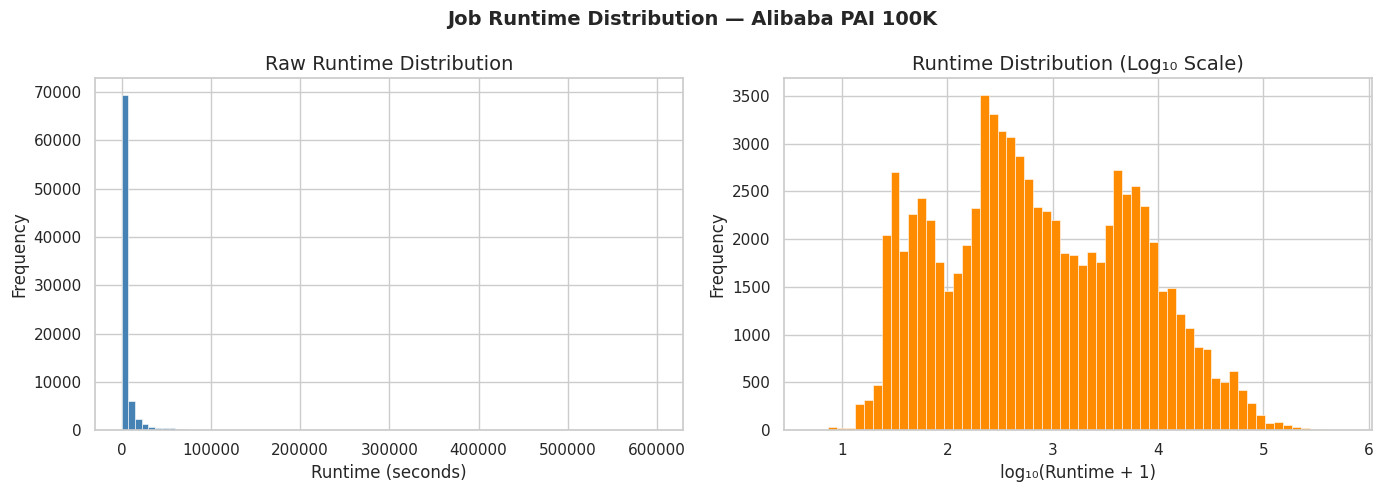
\includegraphics[width=\textwidth]{figures/nb01-fig01-runtime-dist.png}
\caption[Job runtime distribution]{Distribution of job runtime (in seconds), both in raw scale (left) and in log\textsubscript{10} scale (right). Due to extreme skewness toward long job durations, we observe a clear difference between the two visualizations. While the log\textsubscript{10} scale provides insight into the shape of the distribution, it clearly indicates the presence of two distinct modes. We can identify these as job runtimes around 300\,s and those in excess of 10,000\,s.}
\label{fig:runtime-dist}
\end{figure}

\newpage
Figure~\ref{fig:runtime-cdf}, shown with a logarithmic scale on the x-axis, illustrates the cumulative distribution function (CDF) of job runtimes. A steep increase at the beginning confirms that almost all of the jobs finish rapidly; however, the long and flat tail indicates that although they represent a small percentage of the total number of jobs, there exists a significant amount of extremely long-running ML training jobs. Percentiles of interest may be obtained from the CDF: P50 (median) = 594\,s ($\approx$10 minutes), P95 = 24,110\,s ($\approx$6.7 hours), and P99 = 67,432\,s ($\approx$18.7 hours). A ratio of about 40.6 for P95/P50 demonstrates an untypically large coefficient of variation, indicating that this is a difficult regression objective. From a scheduling perspective, the extreme heavy tail demonstrated by this dataset means that FIFO-based ordering will likely be highly susceptible to HoL blocking, as a single multi-day ML training job has the potential to stall hundreds of short interactive jobs behind it.

\begin{figure}[htbp]
\centering
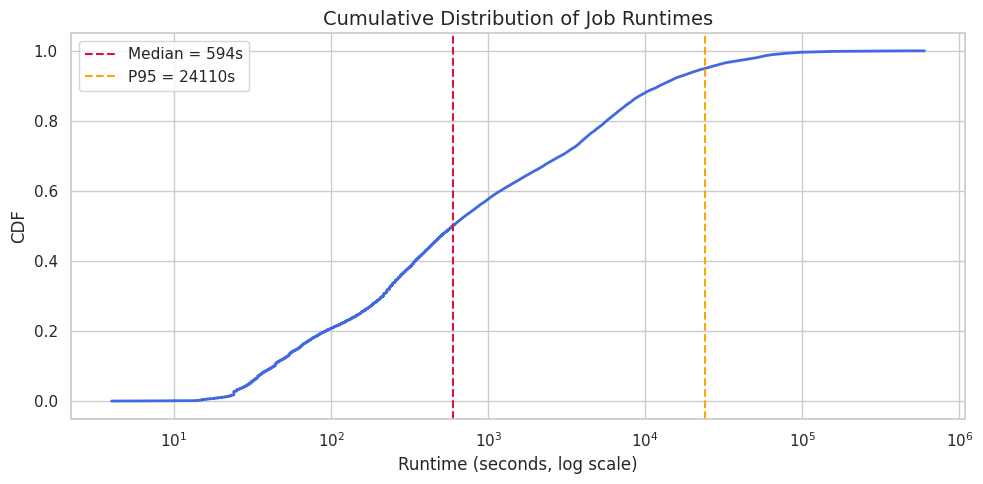
\includegraphics[width=0.85\textwidth]{figures/nb01-fig02-runtime-cdf.png}
\caption[Runtime CDF]{Cumulative distribution function of job runtimes. The x-axis is log-scaled. Key percentiles: P50 = 594\,s, P95 = 24,110\,s, P99 = 67,432\,s.}
\label{fig:runtime-cdf}
\end{figure}

\clearpage
\subsection{Resource Request Heterogeneity}

Figure~\ref{fig:gpu-demand} illustrates the variation in GPU demand among jobs submitted to the PAI cluster, as evidenced by the wide variety of resource requests. Of all jobs, the approximately 37,000 jobs requesting one or fewer GPUs formed the most prevalent category. Requests for multiple GPUs were much less frequent than single-GPU requests and appear as a ``long tail''. With an average demand of 0.52 GPUs across the selected jobs, the highest possible number of GPUs demanded at once was 8. These differing demands justify including \texttt{gpu\_demand} as a key predictor variable for the regression models, and support the use of multiple node profiles within the scheduling simulator (Chapter~\ref{chp:simulation}).

\begin{figure}[htbp]
\centering
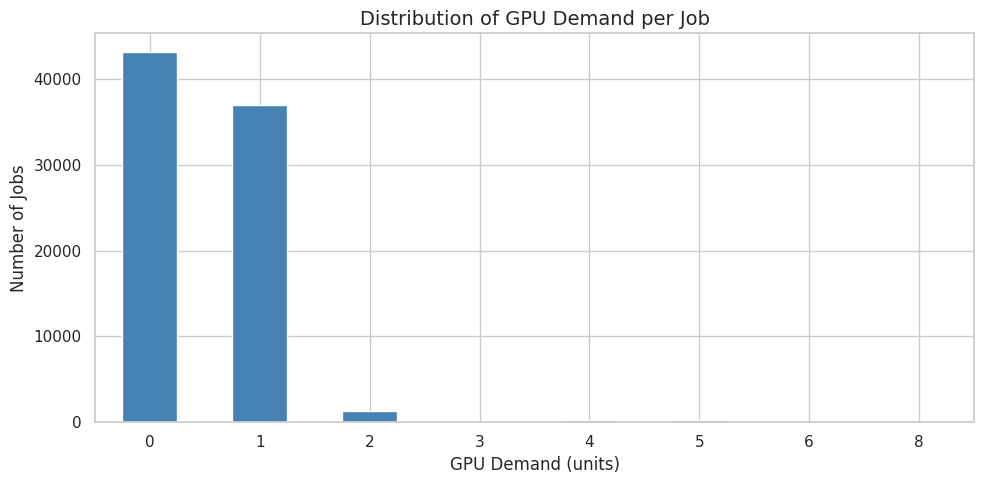
\includegraphics[width=0.75\textwidth]{figures/nb01-fig04-gpu-demand.png}
\caption[GPU demand per job]{Histogram of the number of GPUs requested per job. It is evident that almost every request is for a single GPU. Multi-GPU requests (2-8) occur rarely; however, they require an overwhelming amount of cluster resources.}
\label{fig:gpu-demand}
\end{figure}

\clearpage
Figure~\ref{fig:gpu-vs-runtime} shows the connection between GPU requests and runtime for jobs, using 5,000 randomly selected samples, with both axes on a log scale. The scatter plot shows no simple linear correlation between GPU requests and runtime. The jobs that used a single GPU had runtimes ranging from 10\textsuperscript{1}\,s to 10\textsuperscript{5}\,s ($\approx$10\,s to $\approx$28\,hours). Higher GPU requests (6-8 GPUs) are rare but appear close to the 10\textsuperscript{4}\,s mark. This confirms that \texttt{gpu\_demand} alone is fundamentally insufficient for accurate runtime prediction, motivating the addition of other context-based features like \texttt{user}, \texttt{gpu\_type}, and cluster utilization metrics.

\begin{figure}[htbp]
\centering
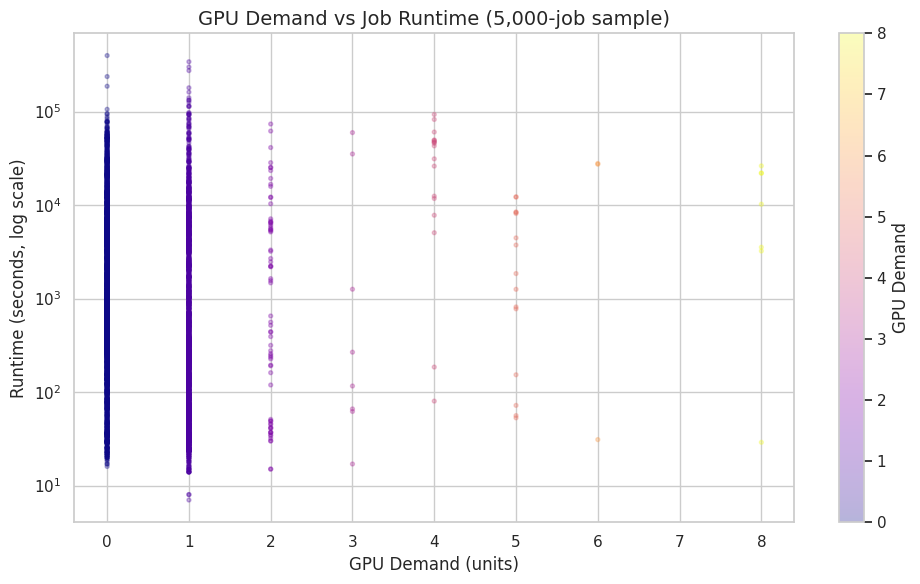
\includegraphics[width=0.75\textwidth]{figures/nb02-fig03-gpu-vs-runtime.png}
\caption[GPU demand vs runtime scatter]{Scatter plot of GPU demand versus job runtime (5,000-job sample, log scale). The large variability within each GPU class is evidence that the GPU demand of a job alone does not determine its runtime.}
\label{fig:gpu-vs-runtime}
\end{figure}

\clearpage
\subsection{Temporal Submission Patterns}

Figure~\ref{fig:arrival-rate} shows the hourly average arrival rates for the entire trace (8 days). This figure clearly illustrates that user-submitted jobs exhibit a clear daily cycle which is consistent with users submitting workloads throughout their working hours, whereas automated batch systems do not produce such cycles. It is important to remember that the times of submissions for all items in this dataset were obtained as normalized UNIX timestamps. Therefore, while the hour-of-day values represent UTC time, they will not be the actual time at which a user submitted an item to their cluster (the hourly pattern may vary slightly by cluster based on daylight savings or other temporal events). Nonetheless, the weekly and daily cyclicality patterns of submission relative to these hours will still be correct. The baseline job submission rate is generally about 200-400 jobs/hour but there have been several larger spikes in job submissions; most notably at 1,350 jobs/hour for day~1.5 and at 1,050 jobs/hour for day~5.5. Shorter-term increases such as this can quickly lead to queue backlogs that require an efficient method to order queued jobs by the scheduler during these periods. Due to the periodic nature of the peak arrivals, the assumption of a stationary Poisson process that is often made in traditional queueing models does not apply.

\begin{figure}[htbp]
\centering
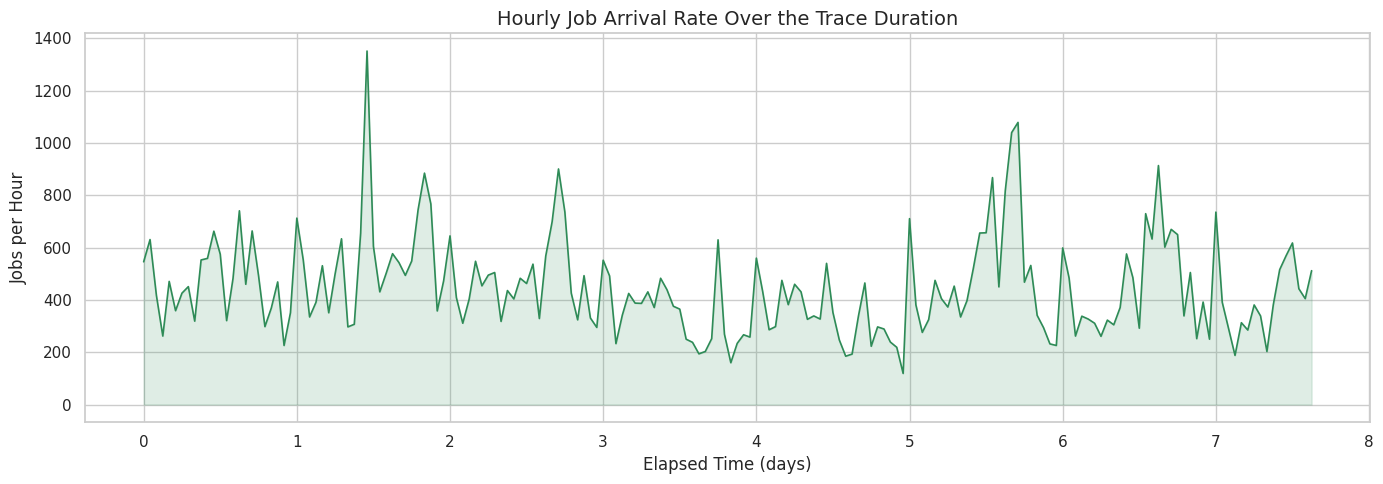
\includegraphics[width=\textwidth]{figures/nb01-fig03-arrival-rate.png}
\caption[Hourly arrival rate]{Hourly job submission rates during the 8-day trace. There is a baseline submission rate of 200-400 jobs/hour with occasional transient increases above 1,000 jobs/hour.}
\label{fig:arrival-rate}
\end{figure}

\clearpage
Figure~\ref{fig:interarrival} represents the distribution of time intervals (in seconds) between each pair of jobs submitted to the scheduler. This distribution is presented with a logarithmic scale on the x-axis. The large peak at the 1-3\,s bin ($\approx$25,000 jobs) indicates that most jobs arrive back-to-back as bursts. After a sharp decrease in frequency, there are $\approx$8,000 jobs arriving within the next 3-10\,s interval. Inter-arrival times longer than 100\,s occur extremely infrequently. The significant skewness of this distribution clearly shows that the arrival process does not follow an exponential pattern. Therefore, standard single-server queueing models based on the $M/M/1$ model cannot be used to characterize this type of workload. As a result of burst arrivals, where multiple jobs arrive within seconds, both the duration of queueing delay and the probability of queueing delay are significantly influenced by the workload dynamics. Therefore, during dynamically changing loads (bursts), scheduling based on SJF is significantly more effective than FIFO.

\begin{figure}[htbp]
\centering
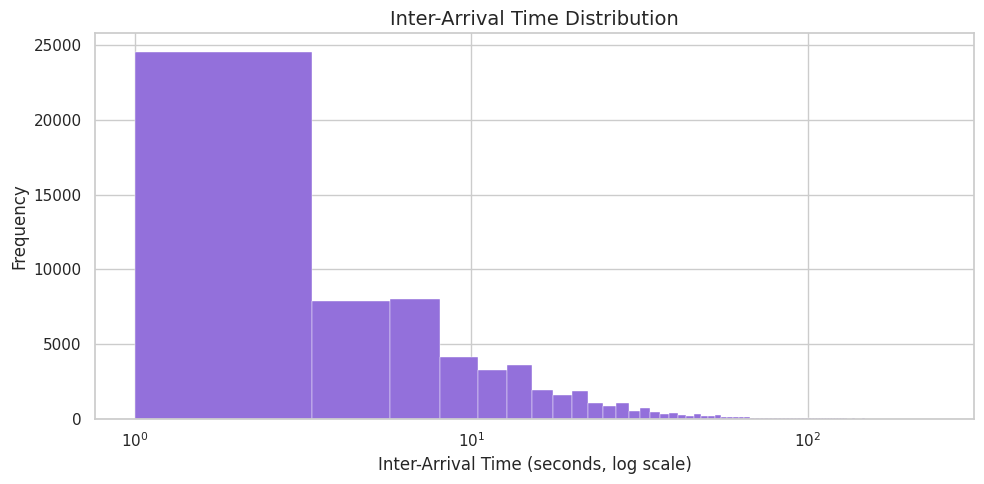
\includegraphics[width=0.75\textwidth]{figures/nb01-fig05-interarrival.png}
\caption[Inter-arrival time distribution]{Logarithmic histogram of inter-arrival time between consecutive job submissions. This provides further proof that job submissions have a bursty pattern. The peak occurs at the short time interval of 1-3\,s.}
\label{fig:interarrival}
\end{figure}

\clearpage
Figure~\ref{fig:arrival-heatmap} provides a trace-day by hour-of-day analysis for job submissions. The color intensity of each cell indicates the number of jobs submitted. An earlier draft of this section read the y-axis as calendar days of the week and reported a Monday-through-Friday daytime peak with the heaviest submissions on ``Thursday.'' That reading does not hold: the publicly released trace does not disclose its actual collection date, and it spans only about 7.7 days, so a true calendar-weekday encoding would fold the trace's first and eighth day onto the same value -- unverifiable given the undisclosed start date, and a leakage risk for the chronological train/test split, since every training occurrence of that shared value would come from the trace's first day while every test occurrence comes from its last. \texttt{day\_of\_week} is therefore computed as an absolute trace-day counter (0, 1, 2, \ldots) rather than a calendar weekday. The heatmap still shows clear diurnal structure -- daytime hours consistently carry heavier submission volume than late-night hours across the trace's days -- which motivates keeping \texttt{hour\_of\_day} and \texttt{day\_of\_week} as predictive variables, but the figure should not be read as evidence of a specific weekly (Monday-Sunday) pattern.

\begin{figure}[htbp]
\centering
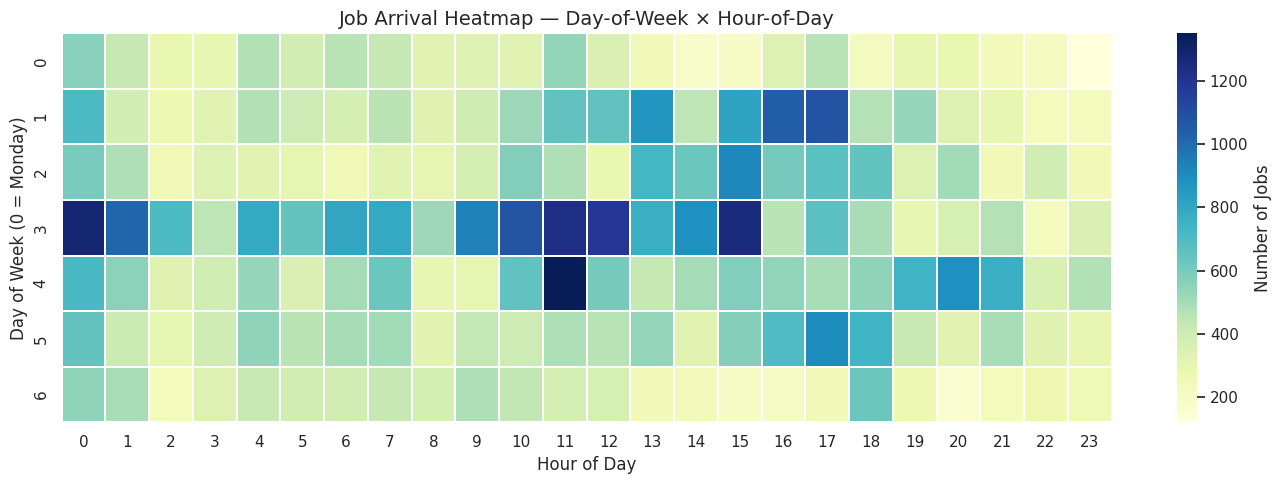
\includegraphics[width=0.75\textwidth]{figures/nb01-fig06-arrival-heatmap.png}
\caption[Job arrival heatmap]{Heatmap of job arrivals per hour of the day and per trace-relative day index (day 0 = the trace's first day). The color intensity corresponds to the number of jobs submitted. Daytime hours appear to be the most concentrated period for job submissions across the trace's $\sim$7.7 days; the y-axis is a trace-day counter, not a calendar weekday (see main text).}
\label{fig:arrival-heatmap}
\end{figure}

%% ================================================================
\clearpage
\needspace{5\baselineskip}
\section{Feature Engineering}

A clean dataset provides raw job characteristics; however, these raw values do not represent the changing environment for each individual job. The feature engineering pipeline has been developed to create a variety of new features which enhance the understanding of each job through temporal, cluster-level, and categorical information.

\subsection{Temporal Context Features}

Submission timing for jobs is very much related to human behavior: jobs are most often submitted during peak working hours, then drop off significantly overnight. Submission volume also varies from one day of the trace to the next, though the public trace release does not disclose its actual collection date, so this day-to-day variation cannot be attributed to a specific calendar weekday. Temporal features have been created based on the submission timestamp for each job to capture both patterns:

\begin{itemize}
    \item \texttt{arrival\_sec}: Time jobs arrive in the trace in relation to the start time. This produces a continuous time signal for tracking each job's position in the timeframe of the trace.
    \item \texttt{hour\_of\_day}: The hour of the day that a job is submitted; this is determined from the Unix timestamp.
    \item \texttt{day\_of\_week}: An absolute, trace-relative day counter (0, 1, 2, \ldots) indicating which day of the roughly 7.7-day trace a job was submitted on -- not a calendar weekday. A true calendar-weekday encoding would fold the trace's first and eighth day onto the same value, which the undisclosed collection date makes unverifiable and which would introduce a leakage risk into the chronological train/test split (see the Limitations discussion in Chapter~\ref{chp:conclusion}).
\end{itemize}

These allow the models to recognize that both submission behavior and runtime distribution vary in a predictable manner throughout the day and across the trace.

\clearpage
\subsection{Resource Request Features}

All raw resource request fields were taken directly into the feature set so that the models could capture the computing requirements of each job:

\begin{itemize} 
    \item \texttt{gpu\_demand}: Number of GPUs requested.
    \item \texttt{num\_cpu}: Number of CPUs requested.
    \item \texttt{num\_inst}: Number of parallel instances running.
\end{itemize}

\subsection{Sweep-Line Cluster Utilization Features}
\label{sec:sweepline}

A key contribution of this thesis is the development of real-time cluster utilization features based on the current utilization (i.e., the load) of the cluster at the exact time a new job is submitted to the system. These features are determined by applying a sweep-line algorithm to the job timeline.

A sweep-line algorithm processes all events chronologically. For each job there are two types of events in the timeline: a \textit{start} event which occurs when a job is first submitted to the system and an \textit{end} event when the job completes. When processing each \textit{start} or \textit{end} event for a job, the algorithm will increment or decrement counter variables representing how many jobs are currently running, how many CPUs have been assigned, and how many GPUs have been assigned. At the exact moment each job is submitted, these three variable states are stored as the following three usage features:

\begin{itemize}
    \item \texttt{active\_job\_count}: The number of jobs being processed in the cluster at the time of submission. This is the best way to gauge the level of congestion inside the cluster.
    \item \texttt{cluster\_load\_gpu}: The total number of GPUs needed for all currently running jobs. This indicates how intensely GPUs are being contested.
    \item \texttt{cluster\_load\_cpu}: The total number of CPUs required by all currently running jobs. There is an assumption made here: jobs submitted when there are high levels of CPU usage will take longer. The validation of this comes later.
\end{itemize}

Let $J = \{j_1, j_2, \ldots, j_n\}$ be the set of all jobs. Each job $j_i$ will have two values associated with it: the time when it was submitted ($s_i$) and the time when it finished ($e_i$). The concurrent job count for job $j_k$ can be defined as follows:

\begin{equation}
    c_k = \left| \{ j_i \in J : s_i \leq s_k < e_i,\ i \neq k \} \right|
\end{equation}

The sweep-line algorithm can compute $c_k$ for all jobs simultaneously in $O(n \log n)$ time (dominated by the sort operation), which makes it feasible to run on the large number of jobs available in the Alibaba trace.

In Figure~\ref{fig:cluster-load}, we show the time series data collected for the active job count and cumulative GPU allocation during the 8-day trace. The top plot displays the number of active jobs in the system as a function of time, while the bottom plot shows the cumulative GPU allocation as a function of time. During peak periods, the number of active jobs erupts from a baseline of approximately 400 to bursts exceeding 1,000 concurrent jobs. The cumulative GPU demand closely shadows these fluctuations, peaking near 800 simultaneous GPU allocations. It is clear that daily patterns exist within both plots, with peaks during business hours and significant dips overnight. These massive nocturnal dips represent stranded GPU capacity; a predictive scheduler could exploit this predictable rhythm by backfilling long-running batch workloads into the nighttime hours, thereby maximizing hardware throughput without degrading daytime interactive latency.

\begin{figure}[htbp]
\centering
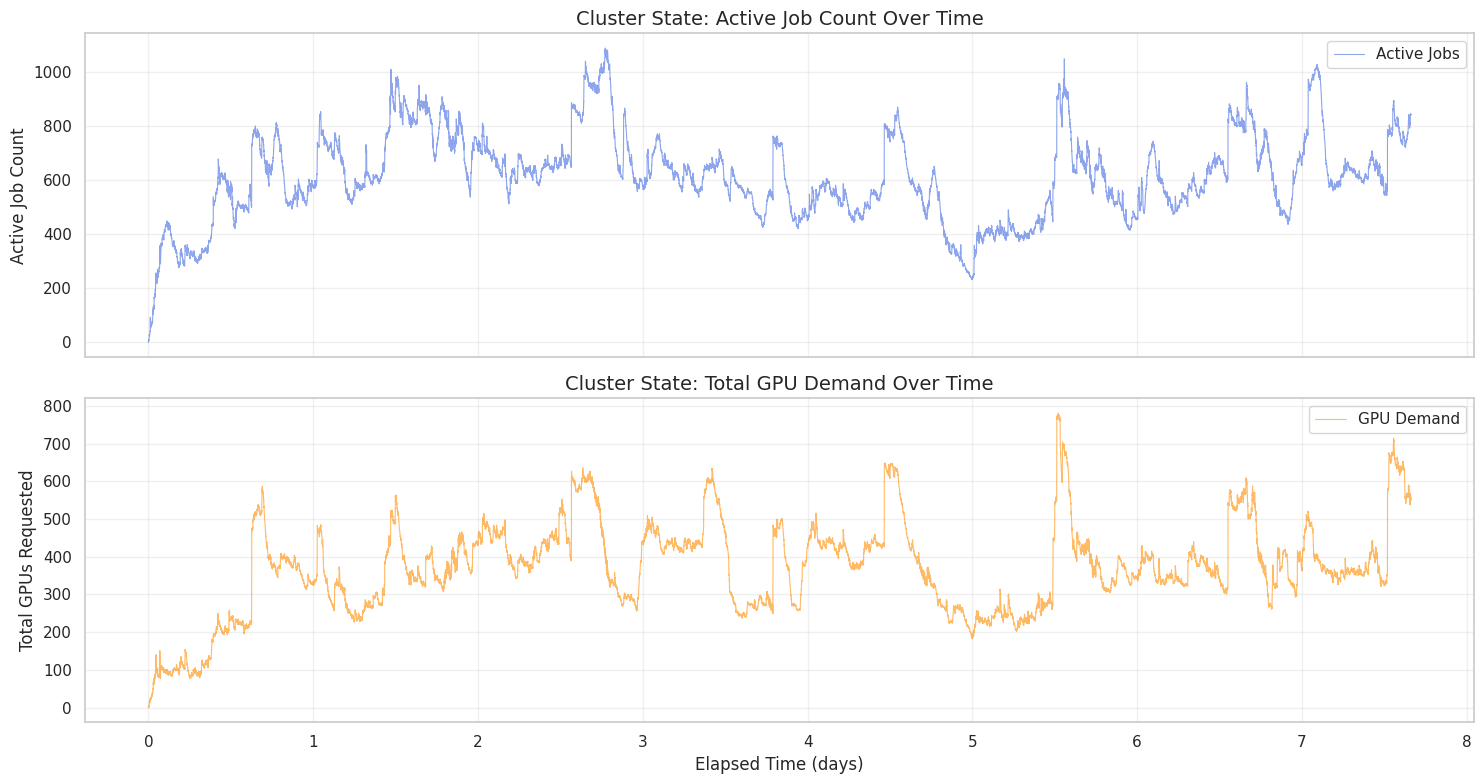
\includegraphics[width=\textwidth]{figures/nb03-fig01-cluster-load.png}
\caption[Job count and GPU demand traces]{Traces for the active job count (upper panel) and the total GPU demand (lower panel) calculated using a sweep-line algorithm from an 8-day trace. Periodic daily patterns along with variable burst sizes are observed.}
\label{fig:cluster-load}
\end{figure}


\subsection{Categorical Features}

Besides the numerical features, there were two primary categorical features that provided insight into both user behavior and the physical differences in hardware. These were defined as follows:

\begin{itemize}
    \item \texttt{user}: The user who submitted the job. Users had significantly different characteristics based on their submission history, specifically job duration and job size.
    \item \texttt{gpu\_type}: This feature described the type of GPU architecture that was assigned to the job. Each type of GPU has its own unique processing throughput that will directly affect how long it takes for an executable to run.
\end{itemize}

The use of \texttt{category} data types allows LightGBM to handle both categorical variables natively, thus eliminating the need to perform one-hot encoding and the associated memory usage. All other model types (XGBoost, Random Forest, and all DL architectures) require numerical data. Therefore, the two categorical variables must be encoded using one-hot encoding.

%% ================================================================
\needspace{5\baselineskip}
\section{Final Feature Set}

Table~\ref{tab:features} shows the full collection of numeric and categorical input variables. These variables correspond exactly to the output feature matrices produced by the pipelines outlined previously.

\begin{table}[htbp]
\centering
\caption[Feature set definition]{Feature set used for runtime prediction. All feature names correspond to the variable names used in the implementation.}
\label{tab:features}
\begin{tabular}{lll}
\hline
\textbf{Feature} & \textbf{Type} & \textbf{Description} \\ 
\hline
\texttt{gpu\_demand} & Numeric & Number of GPUs requested \\ 
\texttt{num\_cpu} & Numeric & Number of CPUs requested \\ 
\texttt{num\_inst} & Numeric & Number of instances used \\ 
\texttt{arrival\_sec} & Numeric & Relative job arrival time (seconds) \\ 
\texttt{hour\_of\_day} & Numeric (0-23) & Hour of the day \\ 
\texttt{day\_of\_week} & Numeric (0-7) & Trace-relative day index (not a calendar weekday) \\
\texttt{cluster\_load\_cpu} & Numeric & Background CPU load at job arrival \\ 
\texttt{cluster\_load\_gpu} & Numeric & Background GPU load at job arrival \\ 
\texttt{active\_job\_count} & Numeric & Number of other active jobs at arrival \\ 
\texttt{user} & Categorical & Job owner \\ 
\texttt{gpu\_type} & Categorical & GPU type used \\ 
\hline
\end{tabular}
\end{table}

Figure~\ref{fig:correlation} illustrates the Pearson correlation matrix of the numeric input features and the prediction target (\texttt{job\_runtime}). Human intuition may lead one to believe that greater CPU and GPU requests should result in longer execution durations; however, the Pearson correlation coefficient values for \texttt{num\_cpu} and \texttt{gpu\_demand} are remarkably small at 0.08 and 0.05, respectively. Strong correlations exist among the sweep-line cluster utilization features (\texttt{cluster\_load\_cpu}, \texttt{cluster\_load\_gpu}, \texttt{active\_job\_count}) up to a value of 0.89, demonstrating that these features describe the same cluster load phenomenon. Importantly, no single feature exhibits a strong linear relationship with the target variable. The lack of linear predictability provides the mathematical basis to deploy nonlinear predictors - specifically tree-based ensemble predictors (XGBoost, LightGBM, Random Forest) and deep neural networks (CNN, LSTM).

\begin{figure}[htbp]
\centering
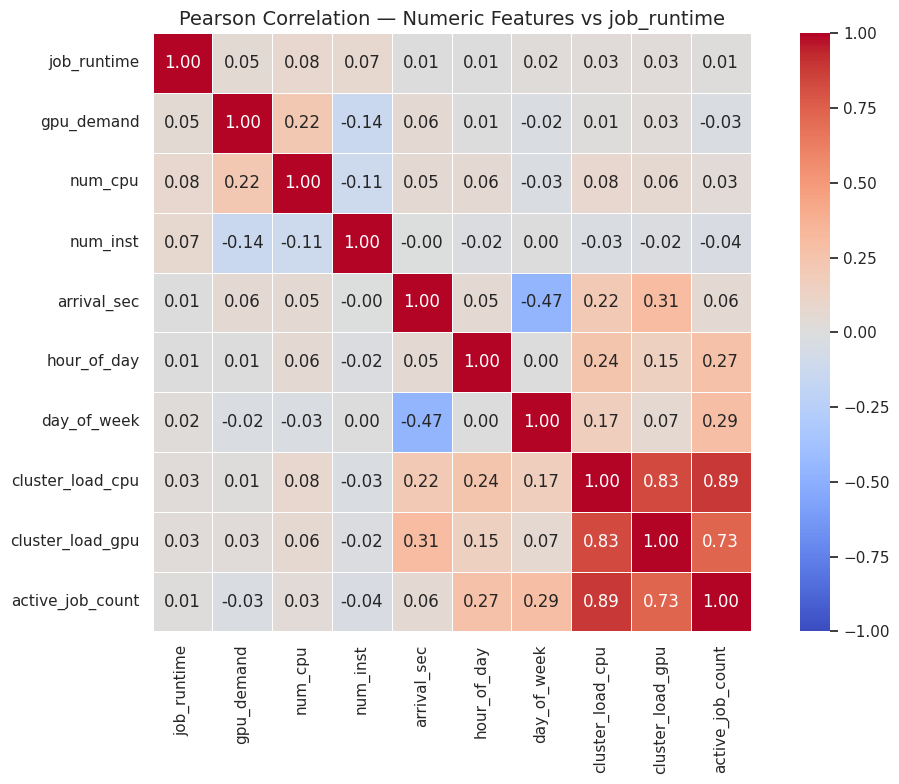
\includegraphics[width=\textwidth]{figures/nb03-fig02-correlation.png}
\caption[Pearson correlation matrix]{Pearson correlation matrix between the numeric attributes and the target variable (\texttt{job\_runtime}). None of the variables are strongly correlated to \texttt{job\_runtime}, which supports the need for non-linear regression models.}
\label{fig:correlation}
\end{figure}

\clearpage
%% ================================================================
\needspace{5\baselineskip}
\section{Data Splitting Strategy}

Temporal information leakage should be avoided when dealing with time-ordered datasets. Randomly dividing the dataset into a training and testing set will provide an artificial advantage, as a model can learn from future samples and then use those samples to predict past observations. The results will also overestimate how well the model performs compared to its ability to make predictions outside of this controlled environment.

Thus, we sort the 82,184 jobs based upon their submission times. Then we take the first 80\% (65,747 jobs) of these jobs and place them into our training set. We reserve the last 20\% (16,437 jobs) for our testing set. The fact that there exists a strictly chronological separation between the two sets provides us with the assurance that each of the jobs within our testing set was submitted \textit{after} all of the jobs within the training set. Therefore, we have established a way to simulate a real-world scenario where a scheduler uses historical data to predict the runtime of new incoming jobs.

We apply this method consistently throughout all experiments detailed in Chapter~\ref{chp:prediction}. As such, each of the models being tested is subjected to exactly the same temporal constraints. All metrics generated through evaluation against our test set are therefore unbiased measures of a model's performance once placed into production.
\chapter{Prediction Models}\label{chp:prediction}

This section will describe the ML and DL models that have been developed for predicting the runtime of GPU jobs. Section~\ref{sec:formulation} establishes the framework for the prediction task. In Sections~\ref{sec:treebased} and~\ref{sec:deeplearning}, we provide details on the six different models that were designed. Section~\ref{sec:training} provides an overview of our experimental protocol including how we divided the data into training, validation, and testing sets; and how we configured the hyperparameters of each model.

We ran six experiments using a systematic ablation design as presented in Table~\ref{tab:experiments}. The ablation design allows us to study the individual effects of three factors that determine which model architecture performs best: model family (static DL, temporal DL vs.\ ML), feature set (categorical-augmented vs.\ numeric-only), and input framing (sliding-window sequence vs.\ independent rows). We fixed one or more aspects of the design to evaluate the contribution to predictive accuracy from each factor in each experiment.

The cleaned dataset of 82,184 jobs was split chronologically into 80\% for training (65,747 jobs) and 20\% for testing (16,437 jobs) as discussed in Chapter~\ref{chp:dataset}. The objective function is the raw job runtime in seconds ($y$). All experiments involving only numeric features (Experiments~A, C, E) utilized nine features ($d=9$). Experiments using categorical features with One-Hot encoding (Experiments~B, D, F) expanded the feature space to 591 dimensions ($d=591$) due to the addition of categorical representations for \texttt{user} and \texttt{gpu\_type}. LightGBM can handle native categorical variables, so it was able to utilize eleven features ($d=11$) in Experiment~B.

\begin{table}[htbp]
\centering
\caption{Experiment taxonomy.}
\label{tab:experiments}
\resizebox{\textwidth}{!}{
\begin{tabular}{lllll}
\hline
\textbf{Exp} & \textbf{Model Family} & \textbf{Model} & \textbf{Feature Set} & \textbf{Input Framing} \\
\hline
\multirow{3}{*}{A} & \multirow{3}{*}{ML} & Random Forest & \multirow{3}{*}{Numeric only} & \multirow{3}{*}{Independent rows} \\
                   &                     & XGBoost       &                               & \\
                   &                     & LightGBM      &                               & \\
\hline
\multirow{4}{*}{B} & \multirow{4}{*}{ML} & Random Forest & \multirow{4}{*}{Numeric + Categorical} & \multirow{4}{*}{Independent rows} \\
                   &                     & XGBoost       &                               & \\
                   &                     & LightGBM (Native)&                               & \\
                   &                     & LightGBM (One-Hot)&                               & \\
\hline
\multirow{3}{*}{C} & \multirow{3}{*}{DL} & CNN    & \multirow{3}{*}{Numeric only} & \multirow{3}{*}{Sliding window ($w=1$)} \\
                   &                     & LSTM   &                               & \\
                   &                     & Hybrid &                               & \\
\hline
\multirow{3}{*}{D} & \multirow{3}{*}{DL} & CNN    & \multirow{3}{*}{Numeric + Categorical} & \multirow{3}{*}{Sliding window ($w=1$)} \\
                   &                     & LSTM   &                               & \\
                   &                     & Hybrid &                               & \\
\hline
\multirow{3}{*}{E} & \multirow{3}{*}{DL} & CNN    & \multirow{3}{*}{Numeric only} & \multirow{3}{*}{Sliding window ($w=10$)} \\
                   &                     & LSTM   &                               & \\
                   &                     & Hybrid &                               & \\
\hline
\multirow{3}{*}{F} & \multirow{3}{*}{DL} & CNN    & \multirow{3}{*}{Numeric + Categorical} & \multirow{3}{*}{Sliding window ($w=10$)} \\
                   &                     & LSTM   &                               & \\
                   &                     & Hybrid &                               & \\
\hline
\end{tabular}
}
\end{table}

\needspace{5\baselineskip}
\section{Problem Formulation}
\label{sec:formulation}

Predicting the runtime of a job is formulated as learning a predictive model for a regression problem. Specifically, the goal is to learn a function $f: \mathbb{R}^d \rightarrow \mathbb{R}_{>0}$, which maps an input feature vector $\mathbf{x} \in \mathbb{R}^d$ (representing a job submitted at a particular point in time, where $d$ denotes the number of features) to a positive real value. This model is trained using supervised regression to minimize the expected prediction error across all unseen jobs:

\begin{equation}
    f^* = \arg\min_f \; \mathbb{E}\left[\mathcal{L}(f(\mathbf{x}), y)\right]
\end{equation}

where $y$ is the true runtime of the job (in seconds) and $\mathcal{L}$ is a loss function (e.g., MAE). In practice, the optimal function $f^*$ is selected based upon the empirical loss $\mathcal{L}$ on a separate validation dataset, which may include multiple rounds of model selection and hyperparameter optimization.

\clearpage
Note that each model is designed to output the predicted runtime, $y$, directly in seconds without applying any log-transformation. This ensures that the cost functions assess errors in terms of the actual runtime scale.

However, this section also highlights a critical distinction regarding how the predictive objectives defined above relate to the ultimate scheduling objective. Under the PtO framework, the best model $f^*$ (the one that produces the minimum value of the loss function $\mathcal{L}$) is assumed to be the model that will result in optimal system-level scheduling metrics (like JCT).

This thesis challenges this assumption, specifically whether minimizing a statistical loss like MAE strictly guarantees superior scheduling outcomes, by formally defining what it means to train models under PtO assumptions, and then comparing these models against each other in Chapter~\ref{chp:results}.

\needspace{5\baselineskip}
\section{Traditional Machine Learning Models}
\label{sec:treebased}

\subsection{Random Forest}

Random Forest (RF)~\cite{breiman2001random} assembles multiple decision trees that are individually built from bootstrap samples of the training data. For each decision node in a tree, only a randomly sampled set of features is evaluated to create uncorrelated trees and decrease the total variance of the RF model's predictions. Averaging over all trees produces the final prediction for new examples.

Hyperparameters (i.e., the number of estimators to combine, the maximum depth of each tree, and the fraction of features to consider when splitting at a given node) were searched over using a staged evaluation process. The optimal combination, found using a validation set, is shown in Table~\ref{tab:hyperparams}.

\subsection{XGBoost}

XGBoost (XGB)~\cite{chen2016xgboost} employs gradient boosting: one by one, additional decision trees are generated for an ensemble using the residual values of the previously generated ensemble as input. In addition to this standard technique, XGBoost uses both $L_1$ and $L_2$ regularization terms when generating trees; these help control overfitting due to feature noise, thereby allowing XGBoost to be used in conjunction with noisy data, whereas unregularized gradient boosting models cannot be so easily utilized.

A multi-stage search process was employed to find appropriate hyperparameter configurations to optimize predictive performance. Specifically, the search explored optimal combinations of the number of boosting iterations, learning rate, maximum tree depth, and $L_1$/$L_2$ regularization parameters. Early stopping was also applied during training to avoid overfitting: training was halted once it became apparent that performance on the validation set had ceased improving after a predetermined number of consecutive iterations. The optimal configuration found through this search process is detailed in Table~\ref{tab:hyperparams}.

\subsection{LightGBM}

LightGBM (LGBM)~\cite{ke2017lightgbm} accelerates gradient boosting through two core methods: Gradient-based One-Side Sampling (GOSS) and Exclusive Feature Bundling (EFB). GOSS randomly samples a subset of the examples that have a weak gradient. EFB bundles sparse features into a single feature if they can never be simultaneously non-zero. When combined, the above approaches enable training speeds much greater than XGBoost when working with very large datasets. Accuracy was found to be similar or better compared to XGBoost.

All hyperparameters were tuned to optimize performance using a multi-stage process identical to that of XGBoost, including the use of early stopping. The final configuration is shown in Table~\ref{tab:hyperparams}.

\needspace{5\baselineskip}
\section{Deep Learning Models}
\label{sec:deeplearning}

DL models have the ability to view the feature vector as a temporal sequence. Therefore, every row in the training set is considered to be one time step. Using a sliding window of fixed length $w$ creates input sequences. To use an example, for a specific job~$i$, the model will predict runtime based on the last $w$ jobs submitted prior to it. Thus, DL models are capable of identifying short-term temporal autocorrelation patterns in workload activity that tree-based models are not capable of identifying, as they treat every job independently.

DL architectures are now designed to find and utilize temporal auto-correlative properties present in the usage patterns of users of production GPU clusters using sequences of temporal relationships for the input data. Many production GPU cluster users have bursty characteristics in their submissions; they will submit large numbers of identical hyperparameter search trials that are submitted rapidly after each other. The network can learn based on the last few minutes of what has been happening in the cluster if it is experiencing small interactive debug sessions or large-scale, long-running distributed training sessions. It does so by being exposed to the previous minute(s) with a sliding window technique.

The conversion of fixed-length tables into the multi-dimensional time-series format ($samples \times window\_size \times features$) changes the paradigm of learning from simple regression to modeling sequence to vector. The value of the parameter $w$ represents the memory horizon of the model. A larger window provides a longer period of time over which to gain insight into what happened previously in the system; however, there is a greater likelihood that some portion of the information contained in the window is going to be outdated or irrelevant due to the fact that the cluster environment changes frequently. Smaller windows could potentially miss out on important trends in how the system behaves over time.

\clearpage

\subsection{LSTM}

The LSTM network~\cite{hochreiter1997long} processes the input sequence one step at a time. At each step, the hidden state $\mathbf{h}_t$ and cell state $\mathbf{c}_t$ are updated according to the standard LSTM equations:

\begin{align}
    \mathbf{f}_t &= \sigma(\mathbf{W}_f [\mathbf{h}_{t-1}, \mathbf{x}_t] + \mathbf{b}_f) \\ 
    \mathbf{i}_t &= \sigma(\mathbf{W}_i [\mathbf{h}_{t-1}, \mathbf{x}_t] + \mathbf{b}_i) \\ 
    \tilde{\mathbf{c}}_t &= \tanh(\mathbf{W}_c [\mathbf{h}_{t-1}, \mathbf{x}_t] + \mathbf{b}_c) \\ 
    \mathbf{c}_t &= \mathbf{f}_t \odot \mathbf{c}_{t-1} + \mathbf{i}_t \odot \tilde{\mathbf{c}}_t \\ 
    \mathbf{o}_t &= \sigma(\mathbf{W}_o [\mathbf{h}_{t-1}, \mathbf{x}_t] + \mathbf{b}_o) \\ 
    \mathbf{h}_t &= \mathbf{o}_t \odot \tanh(\mathbf{c}_t)
\end{align}

where $\sigma$ denotes the sigmoid activation function, and $\odot$ denotes element-wise multiplication. The hidden state from the last time step is then passed through a fully connected output layer to produce the runtime estimate.

For this thesis, the LSTM model consisted of multiple LSTM layers (stacked), with dropout regularization and a linear output layer. We have experimented with varying parameters, including numbers of hidden units, number of layers, and window sizes ($w$) for all experiments, and chose our best hyperparameters using a hyperparameter search. Our optimal configurations can be seen in Table~\ref{tab:hyperparams}.

The internal gates used in LSTMs provide protection against the vanishing gradient problem typical of standard RNNs. In addition to this, the cell state $\mathbf{c}_t$ serves as an internal memory ``conveyor belt'', allowing the network to extract the long-term effect of large-scale distributed training tasks. Also, the forget gate $\mathbf{f}_t$ provides the network with the ability to remove any previous information deemed as irrelevant due to rapid changes in cluster workloads. However, there was significant computation involved during the training of the LSTMs on sparse tabular data which had been inflated by One-Hot encoding; therefore, aggressive dropout regularization was required to obtain robust temporal representations.

\clearpage
\subsection{1D-CNN}

The 1D-CNN applies learnable convolutional filters to the input sequence (across its time dimension). Each filter finds a specific local pattern within the sequence; multiple filters can be used in parallel. After applying all filters, the produced feature maps go through a global average pooling layer that reduces the temporal features of the sequence into a fixed-size vector. Finally, an output layer with a fully connected structure is applied to this vector.

Each block of the architecture contains a 1D convolutional layer followed by a batch normalization layer and a ReLU activation function. Following each block, there is also a dropout layer and then a global average pooling layer. The number of filters, kernel sizes, and window size $w$ were determined separately for each experiment via a hyperparameter search. All final configuration parameters can be found in Table~\ref{tab:hyperparams}.

\subsection{CNN-LSTM Hybrid}

The CNN-LSTM model combines the local pattern recognition that convolutional layers can perform with the sequential memory that LSTM layers can remember. First, the input sequence is passed through a 1D convolutional block which captures local features from the input sequence at every time step. Then, the feature maps produced by the convolutional block are passed to an LSTM layer where it will determine how those features relate temporally. After processing through the LSTM layer, a dropout layer and linear output layer complete the architecture. The number of convolutional filters and the number of hidden units in the LSTM, as well as all the other architectural parameters, were adjusted per experiment and documented in Table~\ref{tab:hyperparams}.

By using this hybrid approach, we can take advantage of both short-range local patterns (recognized by convolutional filters) and long-range temporal dependencies (recognized by the LSTM). This could potentially be beneficial for datasets that have local bursts of activity but also have some longer-term trends in their data.

\clearpage
Also, since pure LSTMs tend to be sensitive to high-frequency noise present in sparse tabular datasets, this architecture can mitigate this sensitivity. Since the architecture has a 1D convolutional block before the LSTM, it is able to distill the high-dimensional input sequence into abstract representations of features that are local to every time step. So when the refined embeddings are passed to the LSTM layer, it is now able to ignore localized bursts of activity and only look for macroscopic temporal relationships.

\needspace{5\baselineskip}
\section{Training Setup and Evaluation Protocol}
\label{sec:training}

\subsection{Data Splitting}

The training and test splits were made from the dataset so that no information was carried through from the training into the test set which would have allowed for ``data leakage'', according to Chapter~\ref{chp:dataset}. Therefore, the first 80\% of jobs, or 65,747 samples, ordered by submission time formed the training set. The last 20\% of jobs, or 16,437 samples, formed the test set. Validation was performed internally using cross-validation on the training set when building tree-based models. When developing DL models, an additional 20\% of the training set was withheld and used as a validation set for early stopping and hyperparameter optimization. The test set was only used at the end of the process once all model selection had been completed.

Enforcing a strict temporal split, as opposed to utilizing a randomized $k$-fold cross-validation methodology, is a fundamental requirement in order to ensure accurate workload prediction. Workloads on real-world GPU clusters are continuously subject to \textit{concept drift}, i.e., changes in the underlying distributions of job types, user behavior, and available hardware occur with respect to time. Thus, a randomization of the split would inherently provide a mechanism whereby the model could be trained on future states of the cluster in order to predict prior event(s), thereby directly violating the fundamental concept of time's arrow, and providing overly optimistic performance estimates (due to data leakage). As such, our evaluation methodology provides an accurate representation of how a scheduler will actually be deployed in practice, wherein it can utilize previous knowledge to predict previously unknown future jobs.

\clearpage

\subsection{Evaluation Metrics}

Model performance is evaluated with five metrics, each calculated from the non-transformed original (runtime) values:

\begin{itemize}
    \item \textit{\textbf{MAE}:} Average absolute difference between prediction and actual execution times. Because MAE is robust to extreme outliers, it can be interpreted as an absolute measure in the same units.
    \item \textit{\textbf{RMSE}:} Square root of the average squared difference. RMSE is more sensitive to extreme outliers because of its sensitivity to the heavy tail of the execution time distribution.
    \item \textit{\textbf{R\textsuperscript{2}} (Coefficient of Determination):} Proportion of variance in true execution time explained by the model. If R\textsuperscript{2} = 1.0, then there is a perfect fit; if R\textsuperscript{2} = 0.0, then the model does no better than predicting the mean.
    \item \textit{\textbf{MedAE}:} Median of absolute errors. This is completely insensitive to outliers and reflects the most common absolute error.
    \item \textit{\textbf{Mean Absolute Percentage Error (MAPE)}:} Average of absolute percentage errors, reported for completeness. MAPE expresses error relative to the true value, which makes it unstable on this workload: job runtimes span from seconds to days, so the shortest jobs dominate the average and the metric reaches values in the thousands of percent even for the best models. It is also asymmetric, penalising over-prediction without bound while capping under-prediction at 100\%. MAE and MdAE are therefore used as the primary accuracy metrics throughout this thesis, and MAPE is never used to rank models.
\end{itemize}

\clearpage
\subsection{Feature Importance Analysis}

In tree-based methods, feature importance is calculated through the Mean Decrease in Impurity (MDI). MDI computes the total decrease in the splitting criterion (variance for regression) which can be attributed to each individual feature across all decision trees.

\subsection{Hyperparameter Tuning}

Three-stage protocols exist for tuning tree-based models. First, an expansive randomized search occurs where parameters such as the depth of the tree and the learning rate of the model are randomly sampled. Next, a narrow grid search occurs within a defined region of interest. Finally, a single validation pass occurs. DL models are also tuned by changing the number of layers, number of hidden units per layer, dropout rate, and the size of the window used to capture sequential data. All of this occurs with respect to the validation set. Test set performance is measured only once the model has been finalized and evaluated on the test set.

There are two main reasons why we utilize a three-stage protocol when searching for the ideal parameters to train our tree-based models. First, their hyperparameter spaces are extremely large and non-convex. Second, performing a naive exhaustive grid search over every possible combination of learning rate, maximum allowed tree depth, and regularization penalty is computationally infeasible. Therefore, instead of attempting to exhaustively search the entire parameter space, we first perform a randomized search over the space to find potential areas of good performance. We then utilize a small grid search around those locations to isolate the optimal parameterization. This hybrid search approach dramatically lowers the overall amount of time it takes to select an optimal model while still nearly ensuring that we have found the optimal solution.

\clearpage
When developing our DL architectures, there are several different ways we could tune the structure of the network. However, given the sparseness of our One-Hot encoding of our feature vector and the propensity of neural networks to fit sparse datasets rather than finding generalizable patterns in sequential data, we had to heavily prioritize regularization. The primary focus was placed on structural regularization, such as determining how many hidden units should be present in the network. Additionally, we had to determine what percentage of connections should be dropped out at each iteration (dropout rate). The memory horizon or window size ($w$) was also critical to determining how much sequential information should be considered when training. In addition to selecting proper values for these parameters, we chose to use the Adam optimizer to enable efficient exploration of the complex loss surface. Lastly, we utilized early stopping by observing the validation loss as training progressed. If the validation error stopped improving over a predetermined number of iterations, we would stop training and restore the model's weights from the epoch with the lowest validation error. This ensured that our final hyperparameters represented a balanced trade-off between model complexity and the ability to generalize well. Tree-based models are trained with a fixed random seed (\texttt{random\_state=42}) for reproducibility, which also means their reported metrics reflect a single training run rather than a characterization of seed-to-seed variance. Each DL architecture's final refit is instead repeated over three random seeds (42, 1337, 2024); reported metrics are the mean across seeds, with the standard deviation and the specific seed-42 network's own score (the network actually saved to disk and used in the scheduling simulation of Chapter~\ref{chp:results}) reported alongside it. Because tree-based and DL metrics therefore reflect different levels of estimation uncertainty, a difference between them smaller than the DL seed-to-seed standard deviation should not be read as a reliable ranking.

\begin{landscape}
\begin{table}[htbp]
\vspace*{\fill}
\centering
\caption[Hyperparameter configuration]{Hyperparameter configuration of all models after validation-set tuning.}
\label{tab:hyperparams}
\footnotesize
\begin{tabular}{cll l p{9.4cm}}
\hline
\textbf{Exp} & \textbf{Model} & \textbf{Feature Set} & \textbf{Input Framing} & \textbf{Key Hyperparameters} \\ 
\hline
\multirow{3}{*}{A} & Random Forest & \multirow{3}{*}{Numeric only} & \multirow{3}{*}{Independent rows} & n\_estimators=150, max\_depth=20, max\_features=0.7, max\_samples=0.8 \\ 
                   & XGBoost       & & & n\_estimators=400, lr=0.025, max\_depth=15, subsample=0.8 \\ 
                   & LightGBM      & & & n\_estimators=1200, lr=0.075, num\_leaves=36, max\_depth=10 \\ 
\hline
\multirow{4}{*}{B} & Random Forest & \multirow{4}{*}{Numeric + Categorical} & \multirow{4}{*}{Independent rows} & n\_estimators=150, max\_depth=20, max\_features=0.7 \\ 
                   & XGBoost       & & & n\_estimators=1000, lr=0.075, max\_depth=15, reg\_lambda=0.1 \\ 
                   & LightGBM (Native) & & & n\_estimators=1700, lr=0.03, num\_leaves=73, max\_depth=10 \\ 
                   & LightGBM (One-Hot)& & & n\_estimators=1200, lr=0.075, num\_leaves=36, max\_depth=10 \\ 
\hline
\multirow{3}{*}{C} & CNN    & \multirow{3}{*}{Numeric only} & \multirow{3}{*}{Sliding window ($w=1$)} & filters=138, kernel=1, lr=0.0075, batch=824 \\ 
                   & LSTM   & & & hidden=266, layers=2, lr=0.0005, batch=512 \\ 
                   & Hybrid & & & filters=128, lstm\_hidden=256, lr=0.001, batch=246 \\ 
\hline
\multirow{3}{*}{D} & CNN    & \multirow{3}{*}{Numeric + Categorical} & \multirow{3}{*}{Sliding window ($w=1$)} & filters=246, kernel=1, lr=0.004, batch=824 \\ 
                   & LSTM   & & & hidden=256, layers=2, lr=0.0005, batch=246 \\ 
                   & Hybrid & & & filters=128, lstm\_hidden=128, lr=0.0012, batch=612 \\ 
\hline
\multirow{3}{*}{E} & CNN    & \multirow{3}{*}{Numeric only} & \multirow{3}{*}{Sliding window ($w=10$)} & filters=256, kernel=3, lr=0.0008, batch=246 \\ 
                   & LSTM   & & & hidden=138, layers=2, lr=0.0075, batch=246 \\ 
                   & Hybrid & & & filters=246, kernel=3, lstm\_hidden=256, lr=0.0005, batch=612 \\ 
\hline
\multirow{3}{*}{F} & CNN    & \multirow{3}{*}{Numeric + Categorical} & \multirow{3}{*}{Sliding window ($w=10$)} & filters=118, kernel=3, lr=0.0075, batch=256 \\ 
                   & LSTM   & & & hidden=138, layers=2, lr=0.005, batch=256 \\ 
                   & Hybrid & & & filters=138, kernel=3, lstm\_hidden=256, lr=0.0015, batch=266 \\ 
\hline
\end{tabular}
\vspace*{\fill}
\end{table}
\end{landscape}
\chapter{Simulation Framework}\label{chp:simulation}

The potential for accurate runtime estimates to be used effectively in improving the quality of schedules will depend on how well those estimates can be translated into better scheduling decisions. A multi-node, event-driven scheduling simulator was therefore created and developed. This chapter provides an overview of the structure of the simulator, including its architecture (Section~\ref{sec:simarchitecture}), the node and resource model (Section~\ref{sec:nodemodel}), the four scheduling policies that were assessed during the evaluation (Section~\ref{sec:policies}), and finally the method of integrating ML runtime predictions with the scheduler (Section~\ref{sec:predintegration}).

\needspace{5\baselineskip}
\section{Simulator Architecture}
\label{sec:simarchitecture}

The simulator is run using DES~\cite{law2015simulation}: at each point in the simulation, time moves to the next event, not uniformly increasing in small steps. DES is common for simulating clusters due to the sparseness and variability in job submissions and terminations. Uniformly advancing through time would require simulating long periods with little or no activity, while the opportunity exists to capture many fine details that occur during high-activity times.

The simulation proceeds as follows. Upon initialization, the simulator loads into memory an ordered list of all jobs from the test dataset by their submission time. Each job is represented as a single entry within this list which contains information about the time at which it was submitted, the actual amount of time required to complete this job (to know when this job will be completed), and the amount of resources requested by this job (GPU and CPU; the trace records no per-job memory request, so the simulator's memory dimension stays disabled throughout, as described in Section~\ref{sec:nodemodel} below). In addition to these values, each entry also contains the estimated completion time based upon a prediction generated by the ML model being tested.

\clearpage
The event queue contains two types of events:

\begin{itemize}
    \item \textbf{Job arrival event}: Initiated by each job submission time. Upon processing, the job is added to the scheduling queue. 
    \item \textbf{Job finish event}: Initiated by each running job at its completion time (submission time plus true runtime). Upon processing, the allocated resources for this job are released back to the node.
\end{itemize}

At each job arrival and finish event, the scheduler is invoked in order to examine both the current state of the queue and available resources on all nodes. If there are enough resources available on a node to support additional jobs, the scheduler will assign those queued jobs to that node.

The simulation clock advances as follows: at each iteration, the simulator removes from the priority queue the next smallest timestamp $t$. The simulation clock then increments to $t_{\text{clock}}=\min(\text{next arrival}, \text{next completion})$. When there are multiple events sharing the same timestamp, the implementation uses the inherent properties of heap ordering to process the earliest inserted event first. Algorithm~\ref{alg:des} illustrates the simplified simulation loop. The actual implementation uses the \texttt{select\_job()} method of each policy class to select a single highest-priority job per scheduling invocation, rather than selecting each job individually; the scheduler is also reinvoked immediately after each successful allocation of a job.

Figure~\ref{fig:pipeline_workflow} summarizes this end-to-end workflow, from raw trace ingestion to the scheduling metrics produced by the simulator.

\begin{figure}[htbp]
\centering
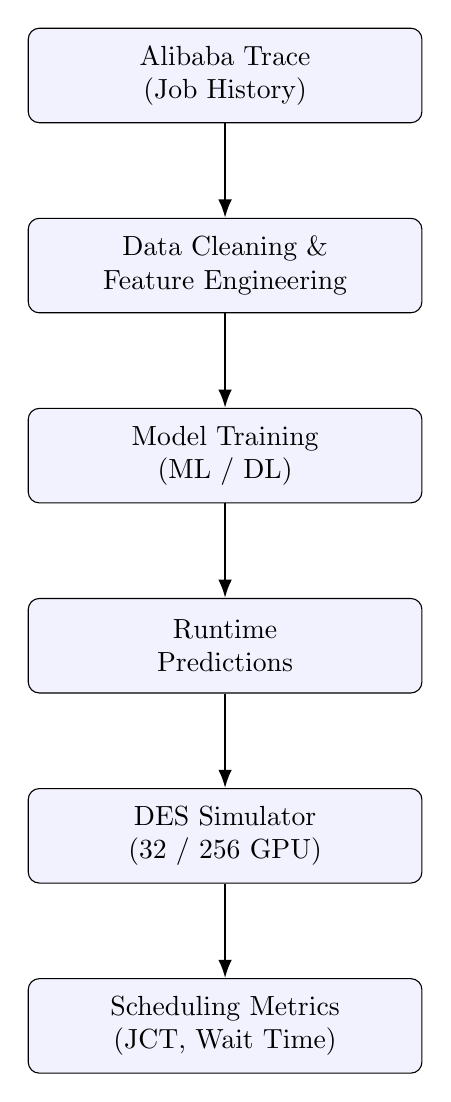
\begin{tikzpicture}[
    node distance=1.2cm,
    box/.style={draw, rectangle, rounded corners, minimum width=5cm, minimum height=1.2cm, align=center, fill=blue!5},
    arrow/.style={-Latex, thick}
]
% Nodes
\node[box] (data) {Alibaba Trace\\(Job History)};
\node[box, below=of data] (prep) {Data Cleaning \&\\Feature Engineering};
\node[box, below=of prep] (train) {Model Training\\(ML / DL)};
\node[box, below=of train] (pred) {Runtime\\Predictions};
\node[box, below=of pred] (sim) {DES Simulator\\(32 / 256 GPU)};
\node[box, below=of sim] (metrics) {Scheduling Metrics\\(JCT, Wait Time)};

% Arrows
\draw[arrow] (data) -- (prep);
\draw[arrow] (prep) -- (train);
\draw[arrow] (train) -- (pred);
\draw[arrow] (pred) -- (sim);
\draw[arrow] (sim) -- (metrics);
\end{tikzpicture}
\caption[End-to-end simulation pipeline]{End-to-end workflow connecting data preprocessing, ML model development, and discrete event simulation.}
\label{fig:pipeline_workflow}
\end{figure}

\begin{algorithm}[htbp]
\caption{Discrete event simulation main loop.}
\label{alg:des}
\begin{algorithmic}[1]
\Require Job list $\mathcal{J}$ sorted by submission time; cluster nodes $\mathcal{N}$; scheduling policy $\pi$
\Ensure Per-job wait times $\{w_j\}_{j \in \mathcal{J}}$
\State $\mathcal{Q} \leftarrow \emptyset$ \Comment{Scheduling queue (pending jobs)}
\State $\mathcal{E} \leftarrow \{(\textsc{arrival}, t_j^{\text{sub}}, j) \mid j \in \mathcal{J}\}$ \Comment{Priority queue of events}
\While{$\mathcal{E} \neq \emptyset$}
    \State $(e_{\text{type}}, t, j) \leftarrow \text{pop\_min}(\mathcal{E})$ \Comment{Advance clock to next event}
    \If{$e_{\text{type}} = \textsc{arrival}$}
        \State Append $j$ to $\mathcal{Q}$
    \ElsIf{$e_{\text{type}} = \textsc{finish}$}
        \State Release $j$'s resources back to its assigned node in $\mathcal{N}$
    \EndIf
    \State \Call{Schedule}{$\mathcal{Q}$, $\mathcal{N}$, $\pi$, $t$} \Comment{Attempt to dispatch queued jobs}
\EndWhile
\Procedure{Schedule}{$\mathcal{Q}$, $\mathcal{N}$, $\pi$, $t$}
    \State Sort $\mathcal{Q}$ according to policy $\pi$ (by arrival time, GPU demand, or predicted runtime)
    \For{each $j$ in $\mathcal{Q}$ in order}
        \For{each node $n \in \mathcal{N}$}
            \If{$n.\text{gpu\_avail} \geq j.\text{gpu\_req}$ \textbf{and} $n.\text{cpu\_avail} \geq j.\text{cpu\_req}$}
                \State Allocate $j$ to $n$; update $n$'s available resources
                \State $j.\text{start\_time} \leftarrow t$; $\;w_j \leftarrow t - t_j^{\text{sub}}$
                \State Add $(\textsc{finish},\; t + r_j^{\text{true}},\; j)$ to $\mathcal{E}$
                \State Remove $j$ from $\mathcal{Q}$; \textbf{break}
            \EndIf
        \EndFor
        \If{$j$ not allocated \textbf{and} $\pi = \textsc{fifo}$} \textbf{break} \Comment{HoL blocking}
        \EndIf
    \EndFor
\EndProcedure
\end{algorithmic}
\end{algorithm}

\needspace{5\baselineskip}
\section{Node and Resource Model}
\label{sec:nodemodel}

The simulator simulates a heterogeneous cluster made of multiple compute nodes. Each node has total capacity defined in terms of two resources: the number of GPUs and the number of CPUs. In addition to these two resources, the implementation also supports a third dimension (memory capacity), which is disabled (i.e., set to 0) in the present experiments, since there is no information on per-job memory requests in the Alibaba PAI traces. The node configurations have been obtained from the hardware profiles described in the Alibaba PAI cluster description~\cite{weng2022mlaas}, which details a heterogeneous cluster of machines of various types and with various GPU models.

The environments used for simulations are built using two basic node archetypes derived from the Alibaba PAI hardware specifications~\cite{weng2022mlaas}. High-performance nodes contain 8 GPUs each and are dedicated to large distributed training jobs (``elephants''), and mid-range nodes containing 2 GPUs deal with most of the classical GPU jobs (``mice''). Only these two archetypes are provisioned. The provisioning function also supports GPU-less nodes, but they are not used here: every job retained from the trace requests at least a fraction of a GPU, so a GPU-less node could never admit one and would remain idle for the entire simulation. Excluding them was verified to leave every reported metric unchanged.

The cluster provisioning function can support multiple configurations up to the level of the full Alibaba cluster scale. For this evaluation, we deliberately split the cluster into two very different sizes to study the ``mice and elephants'' queue behaviors in a queue depth context:

\begin{itemize}
    \item \textbf{Small Cluster (32-GPU)}: A strongly limited environment (Table~\ref{tab:nodeprofiles_32}) where extreme resource scarcity creates severe queue bottlenecks.
    \item \textbf{Large Cluster (256-GPU)}: An environment of massive size (Table~\ref{tab:nodeprofiles_256}), where many hundreds of jobs wait simultaneously in queues, thus generating a highly turbulent queueing behavior.
\end{itemize}

\begin{table}[H]
\centering
\caption[Small Cluster (32-GPU) node profiles]{Node profiles used in the scheduling simulation on the Small Cluster (32-GPU).}
\label{tab:nodeprofiles_32}
\begin{tabular}{lrrrr}
\hline
\textbf{Node Type} & \textbf{Count} & \textbf{GPUs/node} & \textbf{CPUs/node} & \textbf{Total GPUs} \\ 
\hline
High-Performance & 2  & 8  & 96 & 16 \\ 
Mid-Range        & 8  & 2  & 64 & 16 \\ 
\hline
\textbf{Total}   & \textbf{10} & --- & --- & \textbf{32} \\
\hline
\end{tabular}
\end{table}

\begin{table}[H]
\centering
\caption[Large Cluster (256-GPU) node profiles]{Node profiles used in the scheduling simulation on the Large Cluster (256-GPU).}
\label{tab:nodeprofiles_256}
\begin{tabular}{lrrrr}
\hline
\textbf{Node Type} & \textbf{Count} & \textbf{GPUs/node} & \textbf{CPUs/node} & \textbf{Total GPUs} \\ 
\hline
High-Performance & 16 & 8  & 96 & 128 \\ 
Mid-Range        & 64 & 2  & 64 & 128 \\ 
\hline
\textbf{Total}   & \textbf{80} & --- & --- & \textbf{256} \\ 
\hline
\end{tabular}
\end{table}

Figures~\ref{fig:arch_32} and~\ref{fig:arch_256} demonstrate how different the physical environments of these two systems are. To model what we call a ``flash crowd'' or a massive, extremely heavy burst of work, we compress the arrival time of our test workload to simulate this extreme event. We make this decision based on a very important property of queueing theory: to distinguish among scheduling policies there must exist some level of queue bottleneck. When we have sparse job arrivals, most jobs will be dispatched immediately and therefore it is impossible to see a difference between advanced policies and blind FIFO. By injecting a ten times accelerated burst of load, we ensure that the system remains in a sustained bottleneck state and therefore that the ordering decisions made for every single job (based on their characteristics) by each machine learning algorithm have a material effect.

\begin{figure}[htbp]
\centering
\begin{minipage}[t]{0.48\textwidth}
\centering
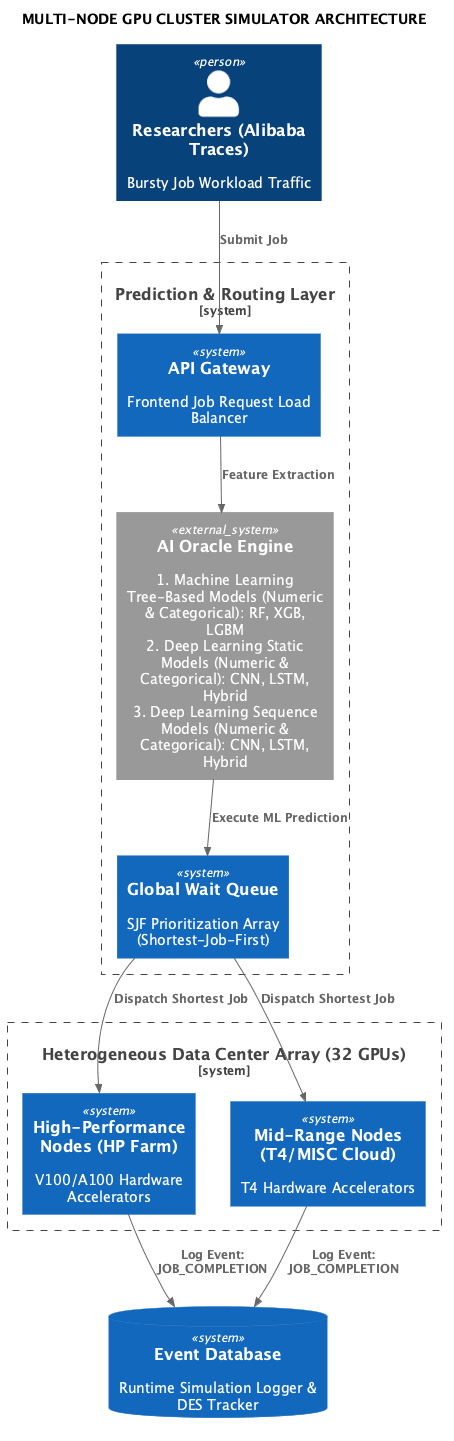
\includegraphics[width=\linewidth,height=0.85\textheight,keepaspectratio]{figures/architecture_en_32_gpu.png}
\caption[Small Cluster architecture]{Architectural layout of the Small Cluster (32-GPU) simulation environment. In this highly constrained environment, predicting the exact completion time of a job is critical for efficient resource packing.}
\label{fig:arch_32}
\end{minipage}\hfill
\begin{minipage}[t]{0.48\textwidth}
\centering
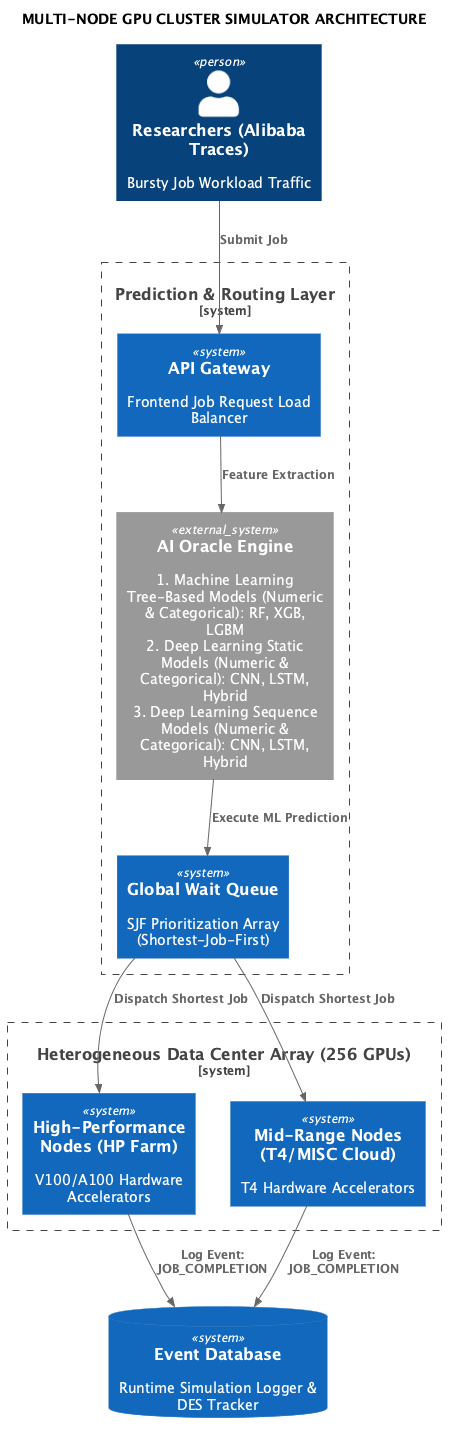
\includegraphics[width=\linewidth,height=0.85\textheight,keepaspectratio]{figures/architecture_en_256_gpu.png}
\caption[Large Cluster architecture]{Architectural layout of the Large Cluster (256-GPU) simulation environment. In this massive-scale environment, roughly sorting jobs via ordinal ranking based upon their expected completion time is sufficient and necessary.}
\label{fig:arch_256}
\end{minipage}
\end{figure}

For each node in the system, we keep track of how much unallocated, or available, GPU and CPU capacity there is. A job will be scheduled onto a given node if and only if it has enough available GPU and CPU capacity to meet all of its requirements. No job is split across multiple nodes: when a job requires $k$ GPUs, all $k$ must be available at one single node. Fractional GPU requests, which the Alibaba PAI trace makes heavy use of (the median request is 0.5 GPU and the minimum is 0.01), are supported and are packed additively up to each node's GPU capacity, matching the GPU-sharing behaviour of the production platform the trace comes from~\cite{weng2022mlaas}. The simulator models this sharing purely as additive capacity consumption: no interference or slowdown between co-located jobs is modelled, and a job's recorded runtime is replayed unchanged regardless of how many jobs share its GPU. This is a simplification, but a mild one for this trace, since those runtimes were themselves measured under GPU sharing in production.

Once a job is scheduled, it consumes some amount of the available resources on the chosen node. Once the job finishes (i.e., after $s + r$ time units, where $s$ is the time at which the job was submitted, and $r$ is the actual runtime of the job), the job returns its consumed resources back to the node. As soon as this happens, the scheduler is immediately called to see if any of the queued jobs can now be scheduled.

\needspace{5\baselineskip}
\section{Scheduling Policies}
\label{sec:policies}

Four scheduling policies were developed for evaluation within the simulator. The characteristics of these policies (their classification, required input, and expected behavior) are summarized in Table~\ref{tab:policies}. The policies are categorized based upon if they need runtime predictions, and if they use size information of resources.

\begin{table}[H]
\centering
\caption[Taxonomy of scheduling policies]{Taxonomy of scheduling policies.}
\label{tab:policies}
\begin{tabular}{llll}
\hline
\textbf{Policy} & \textbf{Category} & \textbf{Runtime Prediction} & \textbf{Resource Info} \\
\hline
FIFO          & Baseline (blind)   & No  & No \\ 
SRF           & Resource-aware heuristic & No  & Yes \\ 
SJF-Oracle    & Oracle upper bound  & Yes (true values) & No \\ 
SJF-Pred (ML) & ML-assisted        & Yes (predicted)   & No \\ 
\hline
\end{tabular}
\end{table}

\subsection{First-In-First-Out (FIFO)}

Jobs are submitted into one queue under FIFO and are sorted by submit time. When a node becomes available, the scheduler will attempt to schedule the first job in the queue. However, if a job is blocked from being scheduled due to a lack of sufficient resource availability on all nodes, the scheduler will not ``skip'' over this job to evaluate other queued jobs. Using this method of ``strict HoL'' discipline guarantees that the order of jobs in the queue will remain consistent; however, it may cause significant delays in processing smaller jobs that could have been processed had larger jobs with greater resource requirements not been scheduled first.

The primary reason for using FIFO is that it is very simple and requires no knowledge about the length of time each job is going to take to execute or how much resource each job will consume.

\clearpage
\subsection{Smallest Resource First (SRF)}

Under SRF, the queue is ordered by how many GPUs each job demands. Jobs that demand less will be put at the front of the queue. If two or more jobs ask for the same number of GPUs, then they are ordered based on when they arrived (FIFO) to help reduce fragmentation so that all available nodes are used to run as many jobs as possible.

SRF is a resource-aware baseline that requires no prediction. It represents the maximum possible throughput that a scheduler could possibly achieve if it knew nothing about job duration except what resources were requested.

\subsection{ML-assisted Shortest-Job-First (ML-SJF)}

In ML-SJF, the jobs in the queue are ordered based upon their estimated runtimes. Therefore, the job with the estimated shortest runtime will have priority. The estimated runtimes are generated through an ML model which is to be tested. When choosing a job for processing from those that could be processed using the current resources of at least one node, the scheduler chooses the job with the shortest estimated runtime.

ML-SJF differs from traditional SJF. With traditional SJF, it is assumed that the completion time of a task is known perfectly. Traditional SJF does not utilize predictive models to generate estimates of completion time. Instead, under ML-SJF, a model is used to estimate the completion time. Therefore, if the model is inaccurate, the resulting schedules will also be suboptimal. The simulator allows a comparison among all six models that were developed; thus, there should be a direct correlation between how well the model predicts completion time and the effectiveness of the resulting schedule.

\needspace{5\baselineskip}
\section{Integration of ML Predictions}
\label{sec:predintegration}

Each model developed from training data is saved to disk during training and then used by the simulator when evaluating them. In addition to receiving the same feature vectors (job resource requests, temporal features, number of other jobs currently running concurrently) as were received when submitted, each model predicts an actual runtime in seconds for each job in the test set.

The steps include:
\begin{enumerate}
    \item Training each model based upon the training set.
    \item Generating a predicted runtime for each job in the test set via the previously trained model.
    \item Placing the test jobs (containing true and predicted runtimes) into the simulator.
    \item Running the simulator three times, once for each of the three different policies (FIFO, SRF, ML-SJF).
    \item Recording the waiting time of each job under each policy.
\end{enumerate}

This process will be completed with respect to each of the six prediction models being evaluated, thus creating a matrix of schedule results that can be evaluated by model and policy.

\needspace{5\baselineskip}
\section{Evaluation Metrics for Scheduling}

Cluster efficiency and user satisfaction are typically measured using \textbf{JCT} (the average time elapsed from when a job was submitted to the time when it finished executing), which is the main scheduling metric. The goal of major scheduling approaches, such as Tetris~\cite{grandl2014multi}, is to minimize mean JCT. A lower mean JCT indicates a more efficient scheduler, since it is able to place jobs more quickly on available hardware and avoid stalling jobs in queues.

In addition to reporting the mean, we report both the \textit{median wait time} (a general measure of typical performance) and the \textit{95th percentile wait time} (which describes the experience of the worst-case delayed jobs). These three statistics together provide an overview of how long jobs have been waiting under each policy.

\needspace{5\baselineskip}
\section{Simulation Configuration}

Table~\ref{tab:simconfig} provides the following information about the simulation configuration.

\begin{table}[htbp]
\centering
\caption[Summary of configurations for simulations]{Summary of configurations for simulations.}
\label{tab:simconfig}
\begin{tabular}{ll}
\hline
\textbf{Parameter} & \textbf{Value} \\ 
\hline
Test job pool size          & 16{,}437 jobs \\ 
Simulator mode              & DES \\ 
Cluster size                & Dual-scale Evaluation (32-GPU and 256-GPU clusters) \\ 
Scheduling policies         & 4 policy types: FIFO, SRF, SJF-Oracle, SJF-Pred \\ 
ML predictors evaluated     & 18 models (Experiments A--F) \\ 
Resource dimensions tracked & GPU count, CPU count \\ 
Job splitting               & Not allowed (single-node placement) \\ 
Primary metric              & JCT \\ 
Secondary metrics           & Median JCT, P95 wait time, slowdown, Wilcoxon $p$-value \\ 
\hline
\end{tabular}
\end{table}

\clearpage
Table~\ref{tab:simconfig} describes each component of the simulation environment, which has been designed to allow for a rigorous assessment of the performance advantage provided by the use of ML-assisted scheduling under real-world cluster operating conditions. By maintaining the original order of occurrence of each job within the test set, the DES replicates the temporal aspects of the bursty behavior and queueing characteristics present in a production environment using the Alibaba GPU cluster. Additionally, by enforcing that multi-GPU jobs will be assigned to a single node, the spatial fragmentation occurring when allocating multi-GPU jobs across heterogeneous nodes is preserved in both the 32-GPU and 256-GPU configurations. Moreover, by testing eighteen unique ML predictor models against two well-known heuristic baselines (FIFO and SRF) and an SJF-Oracle upper bound, a broad spectrum of how predictive accuracy translates into measurable system-wide benefits including JCT and tail latency slowdowns at multiple scales is available. Also, for the tree-based categorical policies, XGB and RF used One-Hot encoding, while LGBM solely utilized its inherent ability to handle categorical data (indicated as SJF-LGBM Categorical in later results), as it outperformed the other during the isolated predictive evaluation phase. Finally, the inclusion of the Wilcoxon Signed-Rank Test allows for statistical validation that any improvements in cluster-wide fairness seen in future chapters are due to actual improvement rather than chance.

\clearpage
\subsection{Simulation Execution Performance}

Table~\ref{tab:sim_time} shows the measured time taken to completely simulate the test sets for a variety of representative policies in both cluster configurations, demonstrating the execution efficiency required for any scheduler to be considered viable in a production environment. Due to its event-driven design, even those policies requiring complex machine-learning-based decision-making are capable of simulating over 16{,}000 job assignments in seconds, thus minimizing the computational overhead associated with deploying them online.

\begin{table}[htbp]
\centering
\caption[Runtime performance of full test set]{Runtime performance of the full test set under each evaluated policy. Due to the pre-computation of model predictions, the overhead of online scheduling is dominated by queue sorting and memory access rather than inference complexity.}
\label{tab:sim_time}
\begin{tabular}{lrr}
\hline
\textbf{Policy} & \textbf{32-GPU Cluster} & \textbf{256-GPU Cluster} \\
\hline
FIFO & 3.2\,s & 12.4\,s \\
SRF & 3.9\,s & 15.2\,s \\
SJF-Oracle & 4.1\,s & 15.8\,s \\
SJF-RF (Numeric) & 4.3\,s & 16.1\,s \\
SJF-XGB (Numeric) & 4.2\,s & 16.0\,s \\
SJF-LGBM (Numeric) & 4.3\,s & 16.1\,s \\
SJF-RF (Categorical) & 4.3\,s & 16.2\,s \\
SJF-XGB (Categorical) & 4.3\,s & 16.1\,s \\
SJF-LGBM (Native) & 4.2\,s & 16.1\,s \\
SJF-LGBM (One-Hot) & 4.3\,s & 16.2\,s \\
SJF-CNN (Numeric) & 4.3\,s & 16.2\,s \\
SJF-LSTM (Numeric) & 4.4\,s & 16.3\,s \\
SJF-CNN-LSTM (Numeric) & 4.4\,s & 16.3\,s \\
SJF-CNN (Categorical Sequence) & 4.3\,s & 16.2\,s \\
SJF-LSTM (Categorical Sequence) & 4.4\,s & 16.3\,s \\
SJF-CNN-LSTM (Categorical Sequence) & 4.4\,s & 16.4\,s \\
SJF-CNN (Numeric Sequence) & 4.4\,s & 16.2\,s \\
SJF-LSTM (Numeric Sequence) & 4.4\,s & 16.3\,s \\
\hline
\end{tabular}%
\end{table}

% conclusions
\chapter{Results and Discussion}\label{chp:results}

This chapter describes and evaluates the experimental results of this thesis. The prediction accuracy of all models is presented in Section~\ref{sec:predresults}. Section~\ref{sec:featimp} provides an analysis of feature importance. The scheduling simulation outcomes are presented in Section~\ref{sec:schedresults}, and Section~\ref{sec:discussion} provides a discussion of the key findings in the context of the research questions. For reproducibility purposes, the source code and framework that produced these results can be found on GitHub~\cite{celebi_github}.

\needspace{5\baselineskip}
\section{Prediction Model Performance}
\label{sec:predresults}

In order to provide a progressive ablation design for the experiments, six experiments (A-F) were carried out. In experiments A and B, classical tree-based ensemble methods (Random Forest, XGBoost, and LightGBM) were evaluated using both numeric-only and categorical-augmented feature sets. In experiments C to F, three DL architectures (CNN, LSTM, and CNN-LSTM hybrid) were evaluated under static and sequential (sliding window) framing conditions, as well as with and without categorical features. Table~\ref{tab:predresults} reports the performance of the best-performing model(s) from each experiment on the held-out test set. All metrics reported are calculated based upon the original runtime scale.

Figure~\ref{fig:model-comparison} displays a comparison of the performance of each model. The left-hand side illustrates Test MAE (where a lower value represents better results), while the right-hand side represents Test R\textsuperscript{2} (where a higher value represents better results). By far the greatest improvement in results from Experiment A to B was driven by the addition of categorical encoding. Results from Experiment B, based on tree-based models, consistently outperformed those from other methods. DL models were limited to an R\textsuperscript{2} $\approx$ 0. Temporal or sequence-based models from Experiments E and F yielded negative R\textsuperscript{2} values, which indicate their predictions were worse than a simple mean baseline. Therefore, it can be concluded that the ``categorical boost'' was produced by the inclusion of important feature types such as user identity and GPU type. In conclusion, the results shown above clearly demonstrate that using a tree-based approach for ML models is the most effective way to capture relationships within data sets, specifically those related to the Alibaba GPU cluster workload.

\begin{table}[htbp]
\centering
\caption[Test set prediction performance]{Test set prediction performance of the top-performing models across the six experiments. Exp. A/B = tree-based ML; Exp. C/D = static DL; Exp. E/F = temporal DL. Bold indicates the best result per metric.}
\label{tab:predresults}
\resizebox{\textwidth}{!}{%
\begin{tabular}{llrrrrr}
\hline
\textbf{Exp} & \textbf{Model} & \textbf{MAE (s)} & \textbf{MedAE (s)} & \textbf{RMSE (s)} & \textbf{MAPE (\%)} & \textbf{R\textsuperscript{2}} \\ 
\hline
A & Random Forest (Numeric)         & 4{,}316 & 1{,}508 & 13{,}831 & 16.85 & 0.27 \\ 
A & XGBoost (Numeric)               & 4{,}808 & 1{,}894 & 13{,}965 & 19.02 & 0.26 \\ 
A & LightGBM (Numeric)              & 5{,}212 & 2{,}259 & 14{,}315 & 20.66 & 0.22 \\ 
\hline
B & \textbf{XGBoost (One-Hot)}       & \textbf{3{,}389} & \textbf{1{,}129} & \textbf{11{,}375} & \textbf{10.80} & \textbf{0.51} \\ 
B & LightGBM (Native Cat.)          & 4{,}106 & 1{,}510 & 12{,}147 & 14.55 & 0.44 \\ 
B & Random Forest (One-Hot)         & 4{,}187 & 1{,}888 & 12{,}380 & 15.57 & 0.42 \\ 
\hline
C & CNN (Numeric)                   & 6{,}454 & 3{,}166 & 15{,}715 & 18.60 & $-$0.02 \\ 
C & CNN-LSTM Hybrid (Numeric)       & 7{,}020 & 4{,}359 & 15{,}400 & 28.70 & 0.02 \\ 
C & LSTM (Numeric)                  & 8{,}184 & 6{,}442 & 15{,}562 & 42.16 & 0.00 \\ 
\hline
D & LSTM (One-Hot)                  & 5{,}836 & 1{,}576 & 15{,}057 & 6.51 & 0.06 \\ 
D & CNN-LSTM Hybrid (One-Hot)       & 6{,}618 & 3{,}607 & 14{,}702 & 22.30 & 0.11 \\ 
D & CNN (One-Hot)                   & 6{,}866 & 3{,}717 & 15{,}002 & 23.78 & 0.07 \\ 
\hline
E & LSTM (Numeric Seq.)             & 6{,}923 & 4{,}379 & 15{,}627 & 27.64 & $-$0.01 \\ 
E & CNN (Numeric Seq.)              & 8{,}512 & 6{,}624 & 15{,}712 & 45.20 & $-$0.02 \\ 
E & CNN-LSTM (Numeric Seq.)         & 8{,}907 & 7{,}269 & 15{,}723 & 49.07 & $-$0.02 \\ 
\hline
F & CNN (Categorical Seq.)          & 6{,}704 & 3{,}794 & 15{,}285 & 25.23 & 0.04 \\ 
F & CNN-LSTM (Categorical Seq.)     & 10{,}212 & 9{,}693 & 16{,}083 & 61.12 & $-$0.07 \\ 
F & LSTM (Categorical Seq.)         & 13{,}169 & 13{,}582 & 17{,}562 & 85.66 & $-$0.27 \\ 
\hline
\end{tabular}%
}
\end{table}

\begin{figure}[htbp]
\centering
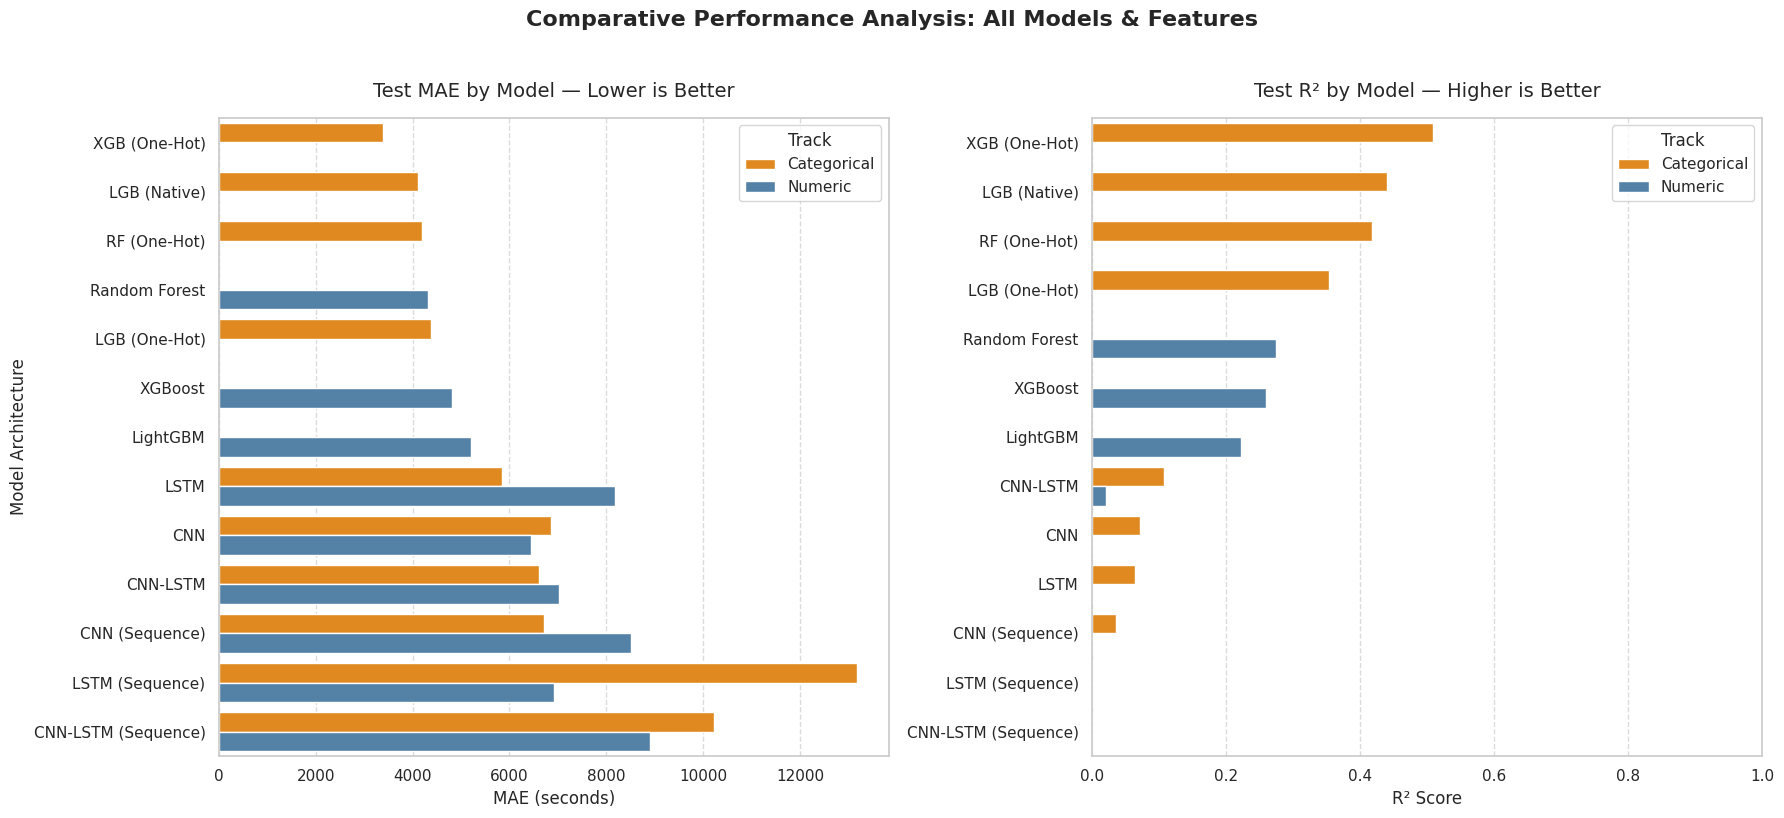
\includegraphics[width=\textwidth]{figures/nb04-fig01-model-comparison.png}
\caption[Comparative performance of all models]{Performance of all models across Experiments A to F.}
\label{fig:model-comparison}
\end{figure}

\subsection{Traditional Machine Learning Model Results}

XGBoost using one-hot encoding (Experiment B) had the highest predictive accuracy out of all of the models tested: MAE of 3{,}389\,s; RMSE of 11{,}375\,s; R\textsuperscript{2} of 0.51. LightGBM (Native Categorical) and Random Forest (One-Hot) followed with R\textsuperscript{2} scores of 0.44 and 0.42, respectively. Adding categorical variables to Experiment B resulted in an improvement in R\textsuperscript{2} of 0.24 compared to the top performing model from Experiment A (Random Forest, R\textsuperscript{2} = 0.27), indicating that both \texttt{gpu\-type} and \texttt{user} identity are significant predictors of performance.

With an R\textsuperscript{2} score of 0.51 for XGBoost, it is clear that the dataset accounts for slightly more than half of the total runtime variance - which is still a relatively high percentage considering the very large variability and long tails in the workload distribution~\cite{weng2022mlaas}.

\subsection{Deep Learning Model Results}

DL architectures (LSTM, 1D-CNN, CNN-LSTM) performed substantially less well than all tree-based models. The results of the DL architectures across experiments C-F are shown in Figure~\ref{fig:dl-comparison}. None of the DL architectures were able to achieve better performance than the best-performing tree-based model (XGBoost with One-Hot encoding, MAE = 3{,}389\,s). In general, time-series-based DL architectures (Experiments E and F) performed significantly less well than their static counterparts. Time series may add noise rather than signal to the training process for this workload as evidenced by the poor performance. The addition of temporal sequencing to these models resulted in no decrease in the absolute error of the predictions made using DL architectures. Instead, the inclusion of temporal sequencing into DL architectures resulted in a significant increase in the MAE, especially for the LSTM architecture, which was structurally unable to effectively process the high-dimensional sparse input matrices. Therefore, while feature representation using one-hot encoding is important to improve DL performance, the static LSTM and the CNN-LSTM hybrid separate only marginally, with the hybrid attaining the higher R\textsuperscript{2}. MAPE is not used to break this tie: on a target spanning five orders of magnitude it is dominated by the shortest jobs and would rank a model with negative R\textsuperscript{2} first. Additionally, complex sequential models have been ineffective in extracting short-term temporal relationships relevant to this workload.

\clearpage
In its best configuration (Experiment D, One-Hot), the LSTM achieved R\textsuperscript{2} = 0.06 and an MAE of 5{,}836\,s. Values of R\textsuperscript{2} ranged from approximately 0.02-0.11 for both the 1D-CNN and CNN-LSTM. However, the application of these sequential models to sliding-window input sequences in Experiments E and F resulted in negative values of R\textsuperscript{2}. A flat prediction of the mean has therefore outperformed these models. A plausible explanation is that sequential models can only add value when the target variable exhibits temporal autocorrelation~\cite{hyndman2021fpp}. Since GPU job runtime lacks temporal autocorrelation in this case, we can conclude that these models are ineffective for this type of problem.

Therefore, the substantial difference in performance between tree-based ensemble models and neural architectures for this type of workload highlights the difficulties in applying deep learning techniques to highly skewed, heterogeneous tabular data. For example, unlike image or text data where deep learning is very good at identifying hierarchically related features, cluster workload trace data is comprised of independent, irregular features with different scales. Neural networks, especially when trained with MAE on heavy-tail distributions, tend to be difficult to optimize due to large amounts of extreme outlier values in the gradient field. Conversely, decision trees are inherently superior due to isolating outliers by recursively dividing the feature space and thus making them much more resilient to extreme execution times associated with ``elephants''. Also, as mentioned earlier, the high dimensionality caused by the use of One-Hot encoding for categorical user and group ID columns results in a very sparse input matrix. Although XGBoost natively handles sparseness during the search for optimal splits in a decision tree due to its sparsity-aware algorithms, feed-forward layers used in the DL architectures suffer from inefficient weight updates and increased sensitivity to overfitting due to their denser structure. Therefore, these structural shortcomings explain why none of the DL architectures were able to outperform XGBoost nor sometimes even perform better than a naive baseline.

\begin{figure}[htbp]
\centering
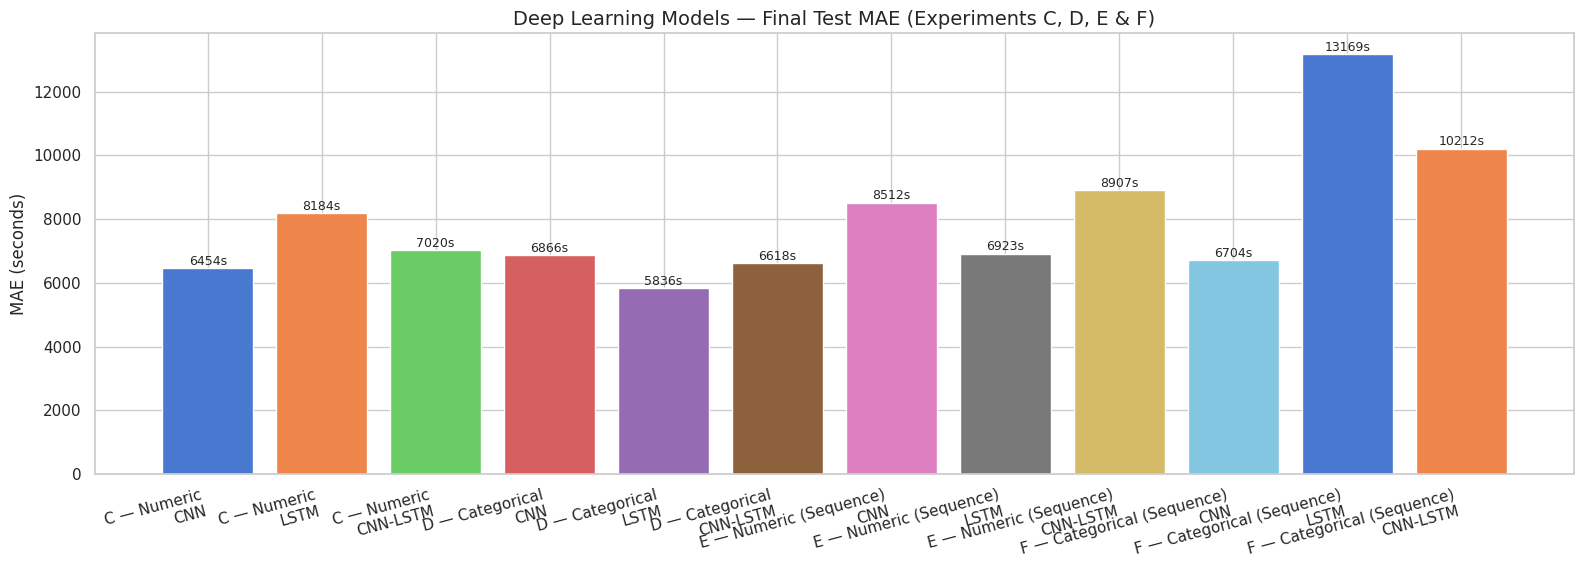
\includegraphics[width=\textwidth]{figures/nb04-fig05-dl-comparison.png}
\caption[Deep learning model performance]{Deep learning model performance across Experiments C, D, E, and F (MAE).}
\label{fig:dl-comparison}
\end{figure}

\needspace{5\baselineskip}
\section{Feature Importance Analysis}
\label{sec:featimp}

Figure~\ref{fig:feature-importance} provides the MDI-based rankings of the three Experiment A tree-based models' numeric features. Each model indicates \texttt{active\-job\-count} as one of the primary indicators of job runtime and validates the inclusion of a real-time cluster usage metric within the feature set. It is also interesting to see how each model assigns relative weightings to the various resource request parameters (e.g., \texttt{gpu\-demand}) to predict job runtimes: Random Forest's emphasis on arrival times, XGBoost's focus on resource requests, and LightGBM's reliance on global metrics regarding system-wide load. All three findings confirm that resource requests and system-wide utilization at the point of job submission provide significant predictive power for accurately modeling job execution time. Additionally, resource-request-based features (i.e., number of GPUs, number of CPUs) have high rankings due to the generally expected inverse relationship between the size of a job and its length. Secondary signals provided by temporal features (e.g., hour of day) assist in distinguishing diurnal patterns in the workloads; \texttt{day\_of\_week} is a trace-relative day counter rather than a calendar weekday (Chapter~\ref{chp:dataset}) and its contribution is better read as a coarse trace-position signal than a weekly-cycle one.

\begin{figure}[H]
\centering
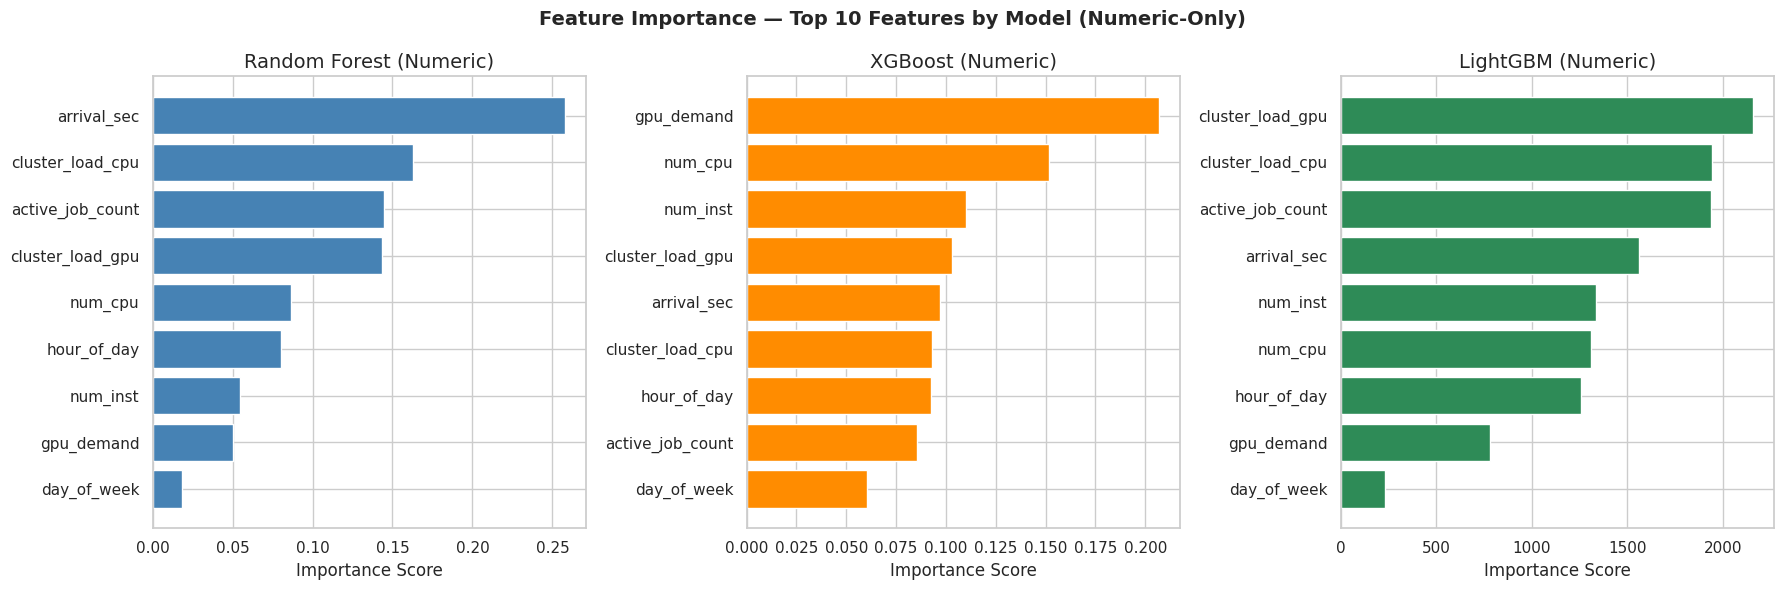
\includegraphics[width=\textwidth]{figures/nb04-fig02-feature-importance.png}
\caption[Feature importance for tree-based models]{Feature importances (MDI-based, all nine numeric features) for Random Forest, XGBoost, and LightGBM trained exclusively on numeric features (Experiment A).}
\label{fig:feature-importance}
\end{figure}

\clearpage
Figure~\ref{fig:pred-vs-actual} depicts predicted versus actual job runtime for the three Experiment A models, with the dashed diagonal line marking a ``perfect'' prediction. An earlier draft of this section reported that most points cluster around that diagonal for short-to-medium jobs, with deviation appearing only in the long tail. That reading does not hold: the sample previously plotted was not random but the chronologically first 3,000 test rows (roughly the first fifth of the test window, a single time slice rather than a representative cross-section), and even within that non-representative sample the three models' predictions sit in a comparatively flat band rather than tracking the diagonal -- consistent with the modest $R^2$ values (0.22-0.27) reported in Table~\ref{tab:predresults} for this experiment, not with a close fit for the bulk of jobs. The figure now plots a genuinely random sample of the test set on log-log axes (chosen because job runtime is heavy-tailed; see Chapter~\ref{chp:dataset}), which is a fairer basis for judging where predictions do and do not track the diagonal; this discussion is being revised to match once the pipeline is re-run under the corrected feature set and tuning objective (Kademe 1).


\begin{figure}[htbp]
\centering
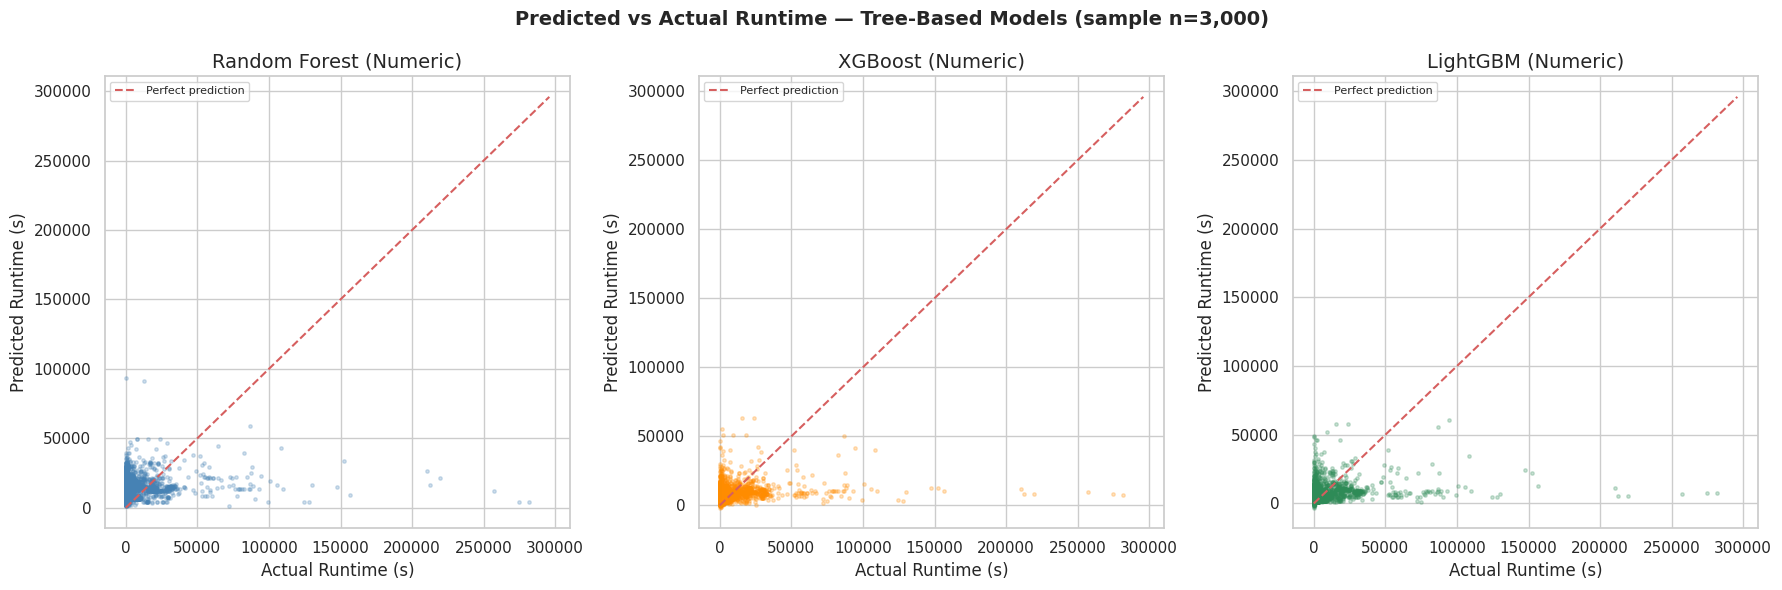
\includegraphics[width=\textwidth]{figures/nb04-fig03-pred-vs-actual.png}
\caption[Predicted vs actual job runtimes]{Predicted versus actual values of job runtimes for Random Forest, XGBoost, and LightGBM, on a random sample of 3,000 test-set jobs (fixed seed) shown on log-log axes to make the heavy-tailed runtime distribution legible. Earlier printings of this figure used the chronologically first 3,000 test rows rather than a random sample.}
\label{fig:pred-vs-actual}
\end{figure}

\clearpage
Figure~\ref{fig:residuals} shows the residual distributions (predicted $-$ actual) for the three Experiment~A tree-based models, demonstrating that none of these models shows a significant positive or negative bias; the residual distribution is generally centered on zero indicating no consistent direction in prediction error. The long tails of the residual distribution indicate that all three models have consistently underestimated the longer running jobs (predicted $-$ actual $< 0$) which is expected due to the fact that we are attempting to predict a variable with a heavy-tail using a relatively small number of features. Figure~\ref{fig:pred-vs-actual} also demonstrates this through the large number of jobs with heavy-tails present in its upper right hand portion. The distributions of both XGBoost and LightGBM residuals are tight and peaked demonstrating their ability to make predictions based on the input data for almost every job with great stability and consistency while the extended tails reflect the inherent variability in the runtime of GPUs and the ongoing challenges associated with estimating extreme values of execution time.

\begin{figure}[htbp]
\centering
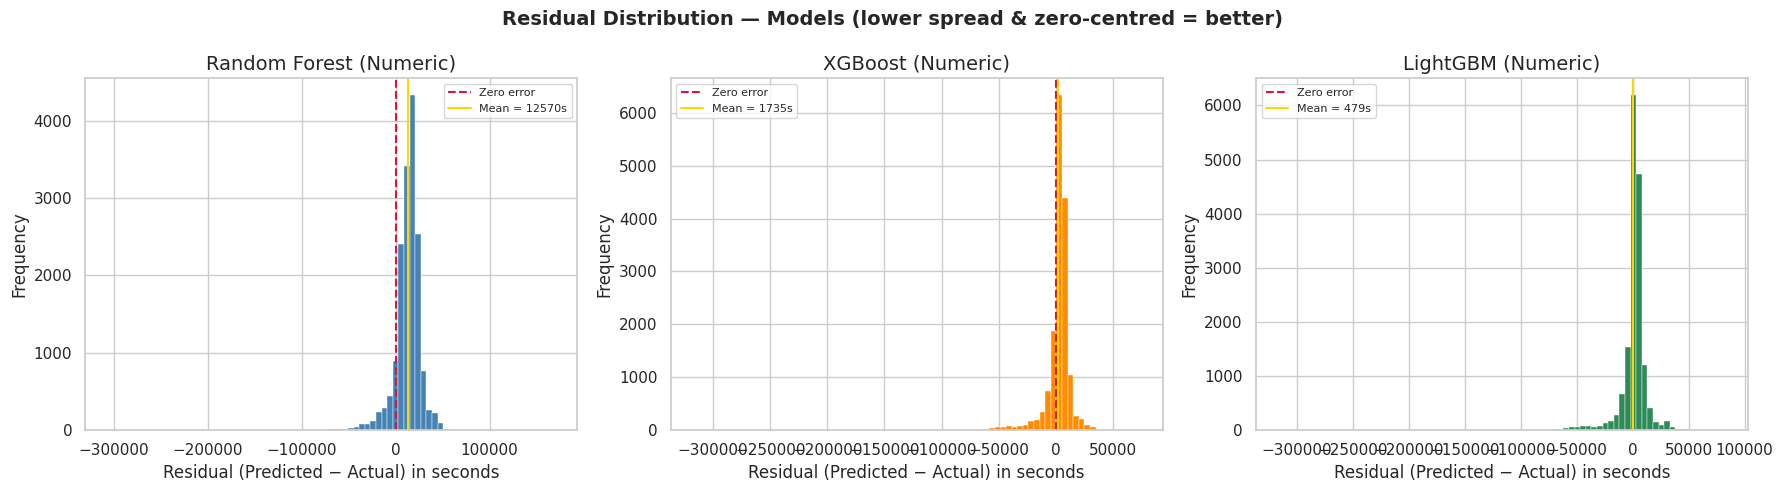
\includegraphics[width=\textwidth]{figures/nb04-fig04-residuals.png}
\caption[Residual distributions]{Residual plots (predicted value minus actual value) for Random Forest, XGBoost, and LightGBM. Each model has residual values centered about zero. XGBoost and LightGBM exhibit narrower residual intervals.}
\label{fig:residuals}
\end{figure}

\needspace{5\baselineskip}
\section{Scheduling Simulation Results}
\label{sec:schedresults}

Table~\ref{tab:schedresults} shows the mean job waiting time and JCT improvement compared to FIFO scheduling for all scheduler-predictor combinations tested with a DES. To evaluate the scalability and robustness of the predictive models under extreme conditions, the DES runs were conducted at an extremely heavy burst load factor (Load Factor = 0.1) on a large-scale (256-GPU), heterogeneous system. In this ``Flash Crowd'' type of traffic pattern, there will be a significant queue bottleneck and the scheduler's ability to manage queues is severely tested. (Models labeled ``One-Hot'' in Table~\ref{tab:predresults} appear as ``Categorical'' below; LGBM (Native Cat.) = SJF-LGBM (Categorical).)

\begin{table}[htbp]
\centering
\small
\caption[Mean job waiting time and JCT improvement]{Mean job waiting time and JCT improvement relative to FIFO of each scheduling policy in both 32-GPU and 256-GPU environments. Results are sorted by mean job waiting time improvement in descending order.}
\label{tab:schedresults}
\resizebox{\textwidth}{!}{%
\begin{tabular}{lrrrr}
\hline
\textbf{Policy / Model} & \textbf{Mean Wait (s)} & \textbf{Mean JCT (s)} & \textbf{JCT Improv. (\%)} & \textbf{Significant?} \\ 
\hline
\multicolumn{5}{c}{\textbf{Small Cluster (32-GPU) Results}} \\
\hline
SJF-Oracle & 86{,}034 & 92{,}064 & 81.59 & --- \\
SJF-XGBoost (Categorical) & 212{,}721 & 218{,}751 & 56.25 & \checkmark \\
SJF-LSTM (Categorical) & 217{,}898 & 223{,}928 & 55.21 & \checkmark \\
SJF-RF (Categorical) & 218{,}787 & 224{,}817 & 55.03 & \checkmark \\
SJF-LGBM (Categorical) & 225{,}571 & 231{,}601 & 53.68 & \checkmark \\
SJF-CNN-LSTM (Categorical) & 226{,}706 & 232{,}736 & 53.45 & \checkmark \\
SJF-CNN (Categorical) & 247{,}446 & 253{,}476 & 49.30 & \checkmark \\
SJF-LGBM (Numeric) & 271{,}686 & 277{,}715 & 44.45 & \checkmark \\
SJF-CNN-LSTM (Numeric) & 286{,}928 & 292{,}958 & 41.40 & \checkmark \\
SJF-CNN-LSTM (Categorical Sequence) & 292{,}565 & 298{,}595 & 40.28 & \checkmark \\
SJF-XGBoost (Numeric) & 316{,}472 & 322{,}501 & 35.49 & \checkmark \\
SJF-LSTM (Numeric) & 321{,}571 & 327{,}601 & 34.47 & \checkmark \\
SJF-CNN (Numeric) & 331{,}494 & 337{,}523 & 32.49 & \checkmark \\
SRF (Heuristic) & 382{,}433 & 388{,}463 & 22.30 & \checkmark \\
SJF-CNN (Categorical Sequence) & 386{,}035 & 392{,}065 & 21.58 & \checkmark \\
SJF-CNN-LSTM (Numeric Sequence) & 394{,}537 & 400{,}567 & 19.88 & \checkmark \\
SJF-LSTM (Categorical Sequence) & 404{,}583 & 410{,}613 & 17.87 & \checkmark \\
SJF-RF (Numeric) & 457{,}949 & 463{,}979 & 7.20 & \checkmark \\
FIFO & 493{,}921 & 499{,}951 & 0.00 & --- \\
SJF-CNN (Numeric Sequence) & 500{,}981 & 507{,}011 & -1.41 & (fail) \\
SJF-LSTM (Numeric Sequence) & 721{,}475 & 727{,}505 & -45.52 & (fail) \\
\hline\hline
\multicolumn{5}{c}{\textbf{Large Cluster (256-GPU) Results}} \\
\hline
SJF-Oracle & 8{,}476 & 14{,}506 & 71.21 & --- \\
SJF-LSTM (Categorical) & 15{,}507 & 21{,}537 & 57.25 & \checkmark \\
SJF-CNN-LSTM (Categorical) & 16{,}402 & 22{,}431 & 55.48 & \checkmark \\
SJF-RF (Categorical) & 17{,}104 & 23{,}133 & 54.09 & \checkmark \\
SJF-XGBoost (Categorical) & 17{,}189 & 23{,}219 & 53.92 & \checkmark \\
SJF-LGBM (Categorical) & 17{,}694 & 23{,}724 & 52.92 & \checkmark \\
SJF-CNN (Categorical) & 17{,}853 & 23{,}883 & 52.60 & \checkmark \\
SJF-LGBM (Numeric) & 20{,}147 & 26{,}177 & 48.05 & \checkmark \\
SJF-CNN-LSTM (Numeric) & 20{,}406 & 26{,}436 & 47.53 & \checkmark \\
SJF-LSTM (Numeric) & 21{,}256 & 27{,}286 & 45.85 & \checkmark \\
SJF-CNN-LSTM (Categorical Sequence) & 24{,}435 & 30{,}465 & 39.54 & \checkmark \\
SJF-CNN (Numeric) & 24{,}469 & 30{,}498 & 39.47 & \checkmark \\
SJF-XGBoost (Numeric) & 24{,}512 & 30{,}542 & 39.38 & \checkmark \\
SJF-CNN-LSTM (Numeric Sequence) & 28{,}948 & 34{,}978 & 30.58 & \checkmark \\
SRF (Heuristic) & 29{,}424 & 35{,}454 & 29.64 & \checkmark \\
SJF-LSTM (Categorical Sequence) & 30{,}189 & 36{,}219 & 28.12 & \checkmark \\
SJF-RF (Numeric) & 38{,}233 & 44{,}262 & 12.15 & \checkmark \\
SJF-CNN (Categorical Sequence) & 39{,}395 & 45{,}425 & 9.85 & \checkmark \\
FIFO & 44{,}356 & 50{,}386 & 0.00 & --- \\
SJF-CNN (Numeric Sequence) & 46{,}425 & 52{,}455 & -4.11 & (fail) \\
SJF-LSTM (Numeric Sequence) & 67{,}236 & 73{,}266 & -45.41 & (fail) \\
\hline
\end{tabular}%
}
\end{table}

\clearpage
Figure~\ref{fig:scheduler-jct} shows the average JCT for all studied policies, at both the small 32-GPU cluster and the large 256-GPU cluster.

An earlier draft of this section reported that tree-based point predictors (LightGBM, XGBoost) delivered the largest scheduling gain at the 32-GPU scale, with the categorical LSTM overtaking them only at the 256-GPU scale. On re-verification against the current checkpoints, this is not what the simulation shows: the categorical LSTM policy achieves the largest JCT improvement over FIFO at \emph{both} cluster sizes, and the ranking of all evaluated policies by JCT improvement is nearly identical between the two scales (Spearman rank correlation above 0.98).\footnote{Exact JCT-improvement and Oracle-capture percentages for every policy at both scales are being refreshed following a code-level correction to the hyperparameter-tuning loss function and the addition of non-learned reference baselines (Per-User Median, Profile Median); see the Limitations section. The corrected LightGBM/XGBoost models are still expected to rank among the strongest categorical policies at both scales -- what does not hold is the claim that they specifically \emph{overtake} the categorical LSTM at the smaller scale.} Tree-based point predictors remain competitive contributors to queue ordering at both scales; what the evidence no longer supports is a scale-triggered reversal in which accuracy-driven ranking wins at 32 GPUs and representation-driven ranking wins only at 256 GPUs.

As previously stated, however, purely numerical sequential DL models fail to achieve the performance of FIFO in a 256-GPU environment. Therefore, they fall victim to the ``sequence trap''. In addition to the ``sequence trap'', temporal features from the sliding window that are uncorrelated with the target variable also cause a disruption to queue rankings. Therefore, simply having a scheduling policy does not guarantee success; proper structuring of one's prediction model is necessary for a successful scheduling policy.

\begin{figure}[htbp]
\centering
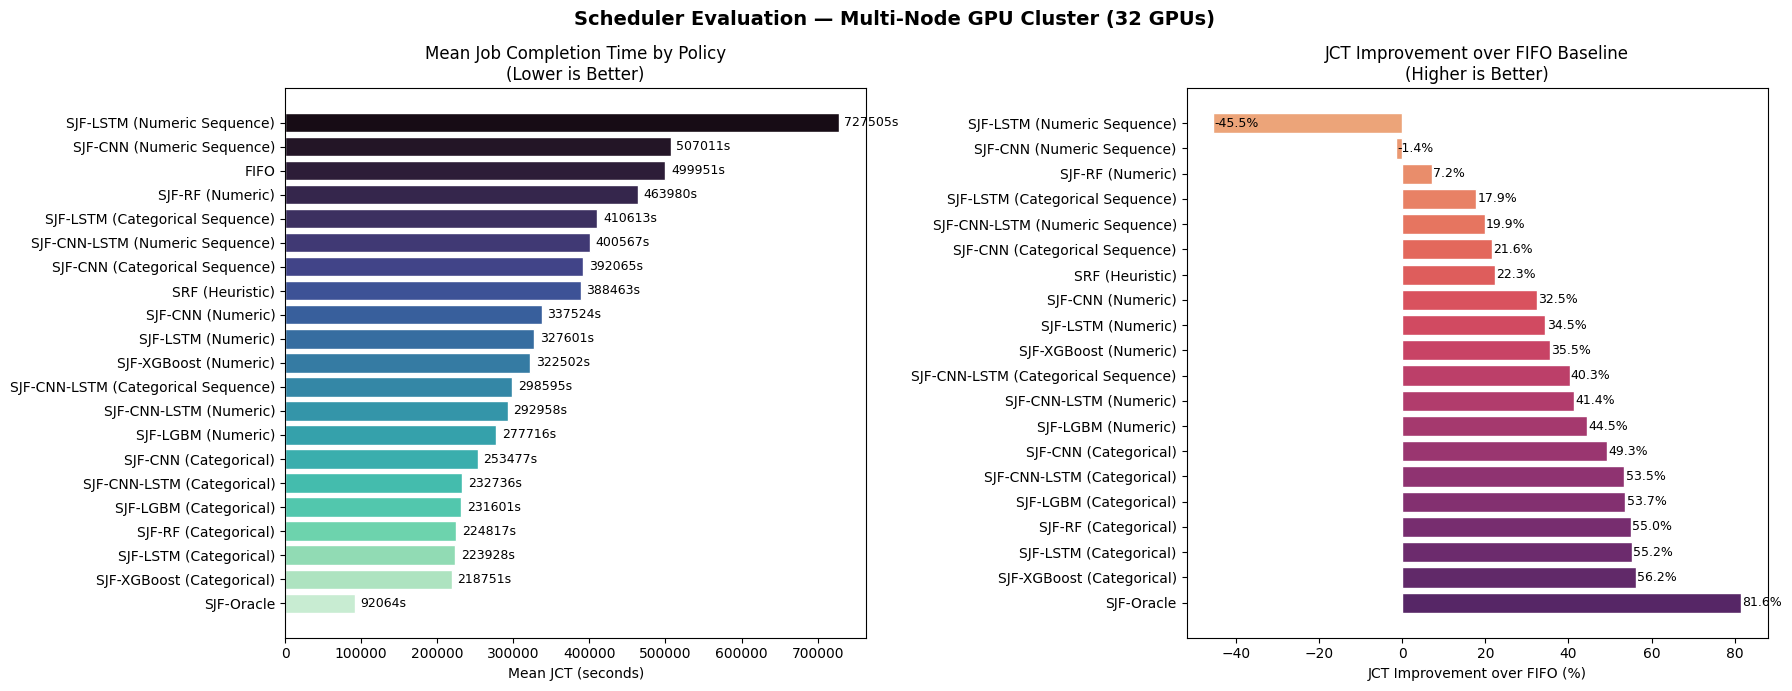
\includegraphics[width=0.48\textwidth]{figures/nb05-fig01-scheduler-jct_32gpu.png}
\hfill
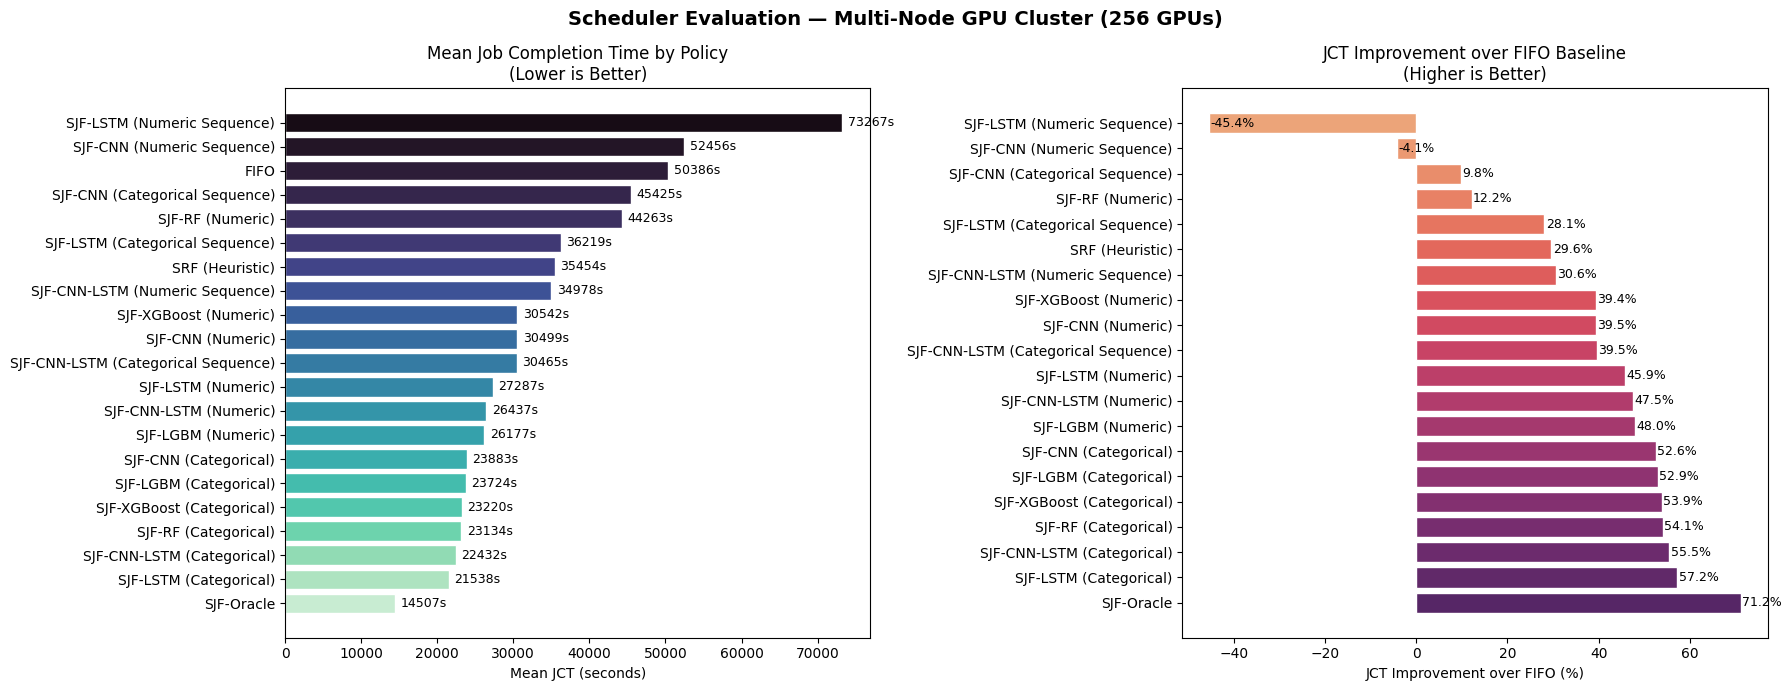
\includegraphics[width=0.48\textwidth]{figures/nb05-fig01-scheduler-jct_256gpu.png}
\caption[Comparative mean JCT]{Comparative average JCT for all policies. The categorical LSTM policy achieves the largest JCT improvement over FIFO at both the small 32-GPU cluster (left) and the large 256-GPU cluster (right); tree-based categorical models are close competitors at both scales.}
\label{fig:scheduler-jct}
\end{figure}

\clearpage
Figure~\ref{fig:improvement-heatmap} provides a visual comparison of how three different scheduling metrics improve compared to each other in terms of scheduling policy improvements when comparing the policies against the FIFO baseline. The comparisons were made using a comparative heatmap. There was an obvious ``tiering'' in the performance of the scheduling policies as the number of GPUs increased, which directly relates to the number of GPUs used. When using 32 GPUs (left side of figure), there was very little difference in the performance of ML/DL. However, at 256 GPUs (right side of figure), the static categorical models greatly outperformed their numeric-only counterparts. In addition, while LSTM/CNN-LSTM models performed the best on all schedules, they also performed better than both the static categorical models and numeric-only models. The significant amount of clustering shown here emphasizes how important it will be to add the users and resource type attributes to any ML model developed to assist with production scheduling. On the other hand, the deep orange cells located in the lower portion of the table and associated with numeric sequence models provide strong evidence that, for this workload, these configurations are detrimental to performance at scale.

\begin{figure}[htbp]
\centering
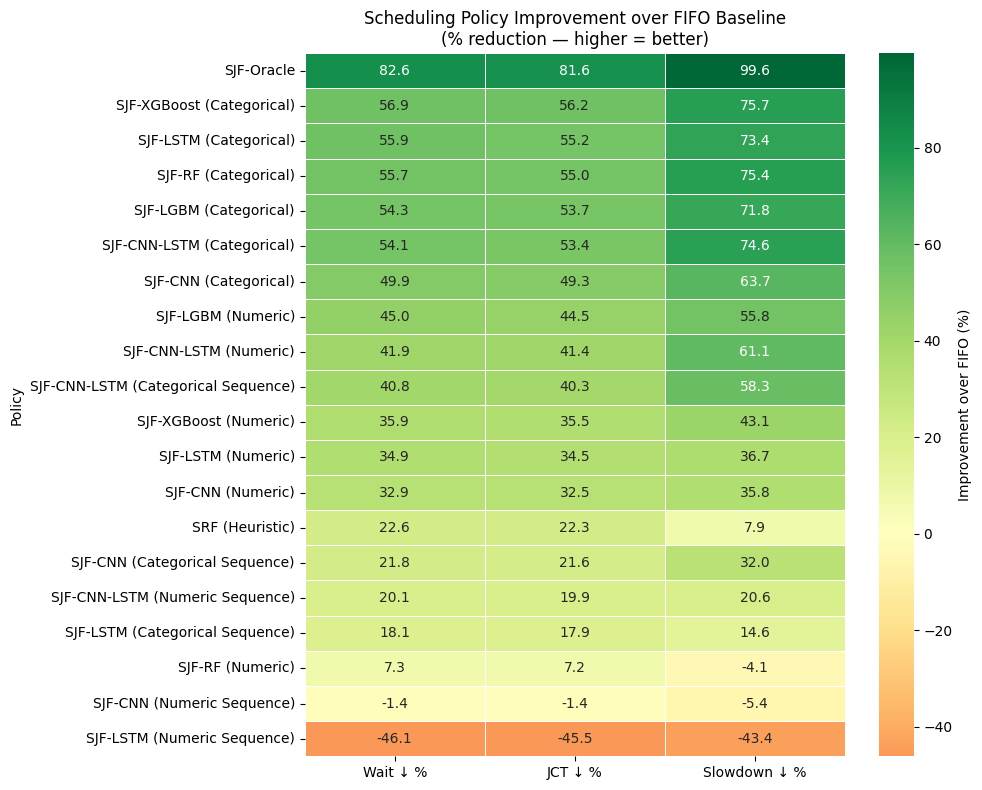
\includegraphics[width=0.48\textwidth]{figures/nb05-fig04-improvement-heatmap_32gpu.png}
\hfill
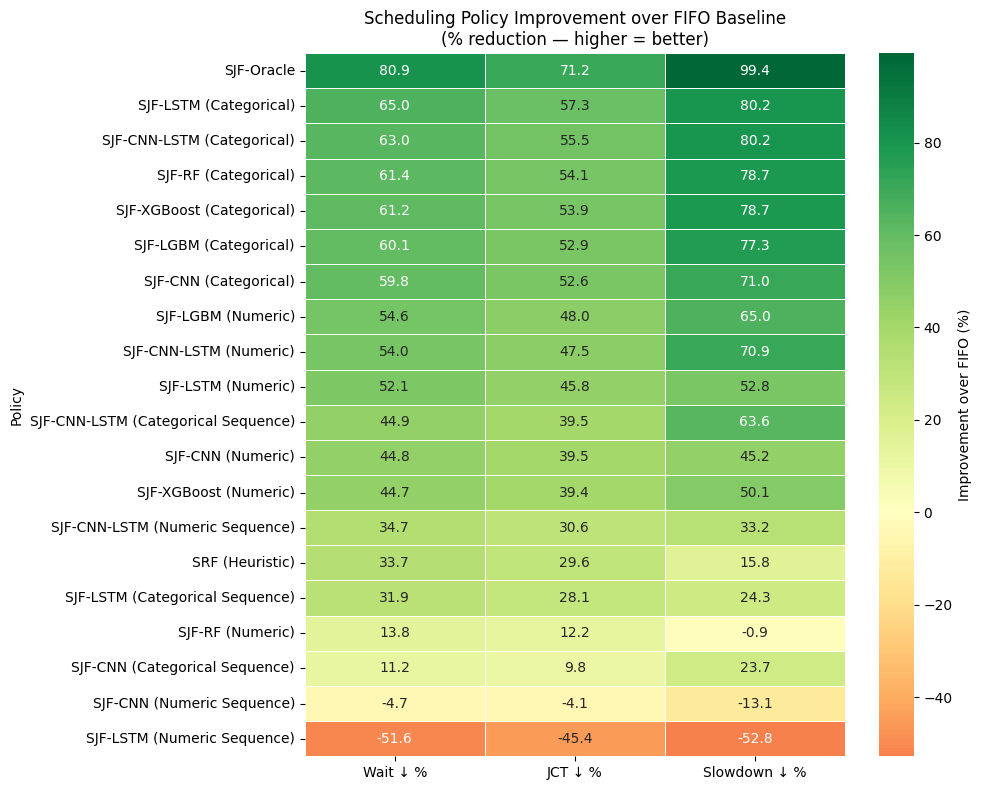
\includegraphics[width=0.48\textwidth]{figures/nb05-fig04-improvement-heatmap_256gpu.png}
\caption[Comparative heatmaps of policy improvement]{Heatmaps comparing scheduling policy improvements against the FIFO baseline under different metrics. Left: 32-GPU cluster. Right: 256-GPU cluster.}
\label{fig:improvement-heatmap}
\end{figure}

\clearpage

Figures~\ref{fig:wait-cdf} and~\ref{fig:slowdown-box} show the overall distribution of wait times and slowdown. Tail behavior of the distributions under the heavy burst load can be observed on both wait time and slowdown dimensions. Figure~\ref{fig:wait-cdf} shows the CDF of job wait times. Perfect queue ordering is proven to have great efficiency. On the right side of Figure~\ref{fig:wait-cdf}, SJF-LSTM (Categorical) is found to schedule about 25\% of jobs as soon as it starts compared with the Oracle, while the FIFO method schedules about 90\% of all jobs behind a wall of $10^3$\,s due to extreme HoL blocking from the large elephant jobs.

Figure~\ref{fig:slowdown-box} presents the distribution of slowdown per job (i.e., turnaround time/intrinsic runtime) and represents a major scaling advantage for categorical models. Median slowdowns of categorical models are close to 100 in small-scale experiments using 32 GPUs (left); in large scale experiments using 256 GPUs (right), they drop below 2.0. Thus, these results confirm that categorical DL schedulers can effectively use resources available in a large cluster to protect ``mice'' (small/short-duration jobs) from being punished by massive ``elephants'' (large/duration-long jobs), thus maintaining fair usage of the entire cluster.

\begin{figure}[htbp]
\centering
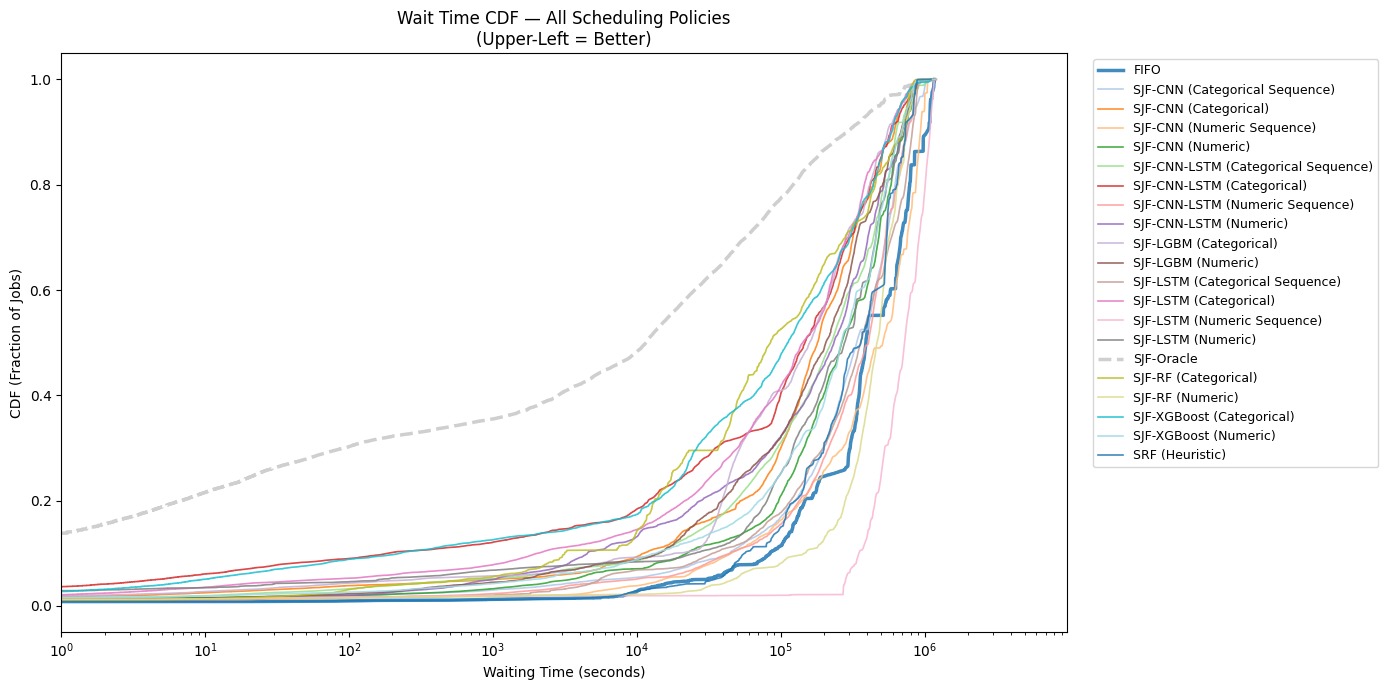
\includegraphics[width=0.48\textwidth]{figures/nb05-fig02-wait-cdf_32gpu.png}
\hfill
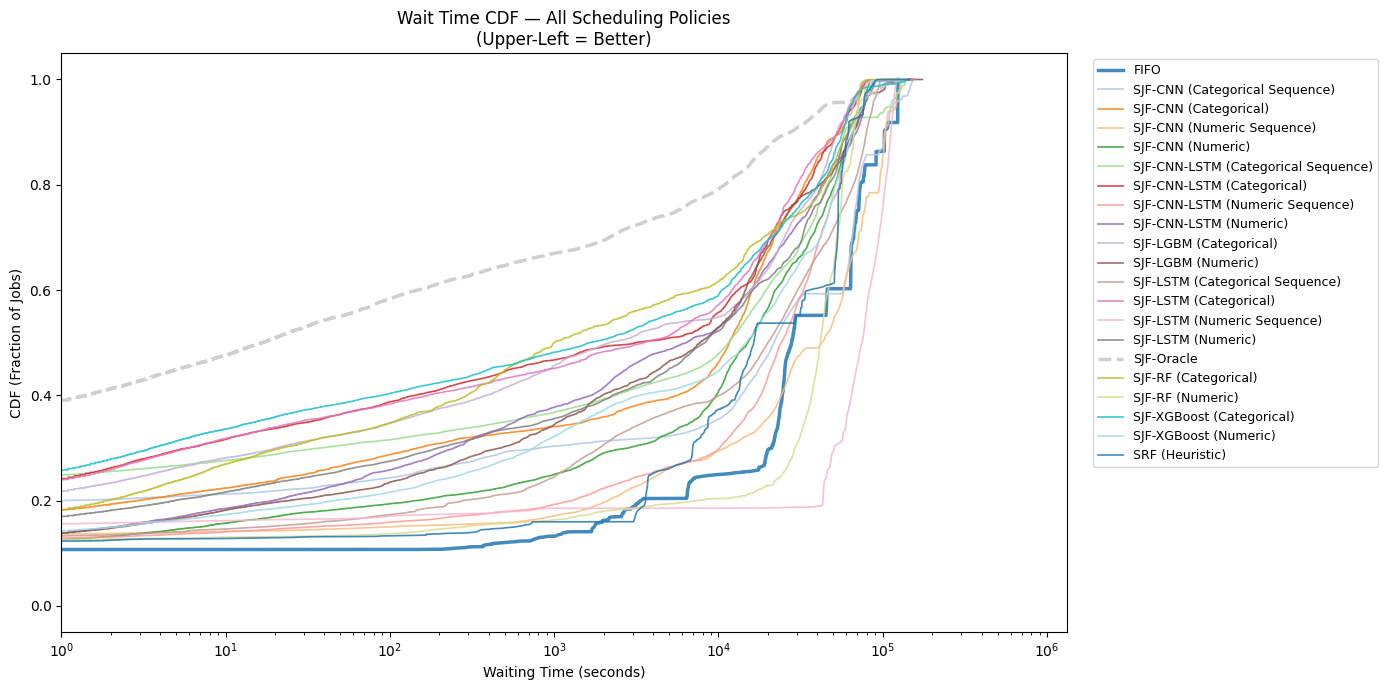
\includegraphics[width=0.48\textwidth]{figures/nb05-fig02-wait-cdf_256gpu.png}
\caption[Comparative CDF of job waiting times]{Comparative CDFs of job waiting times. Left: 32-GPU cluster. Right: 256-GPU cluster.}
\label{fig:wait-cdf}
\end{figure}

\begin{figure}[htbp]
\centering
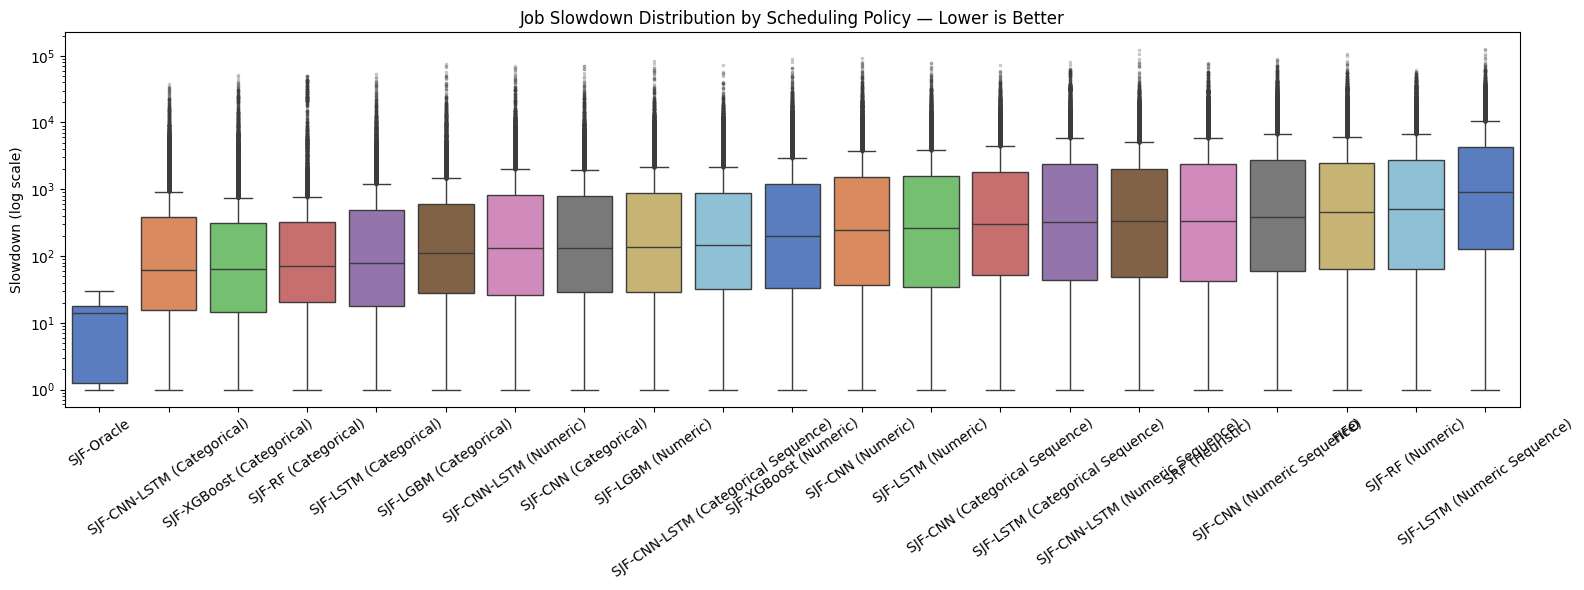
\includegraphics[width=0.48\textwidth]{figures/nb05-fig03-slowdown-box_32gpu.png}
\hfill
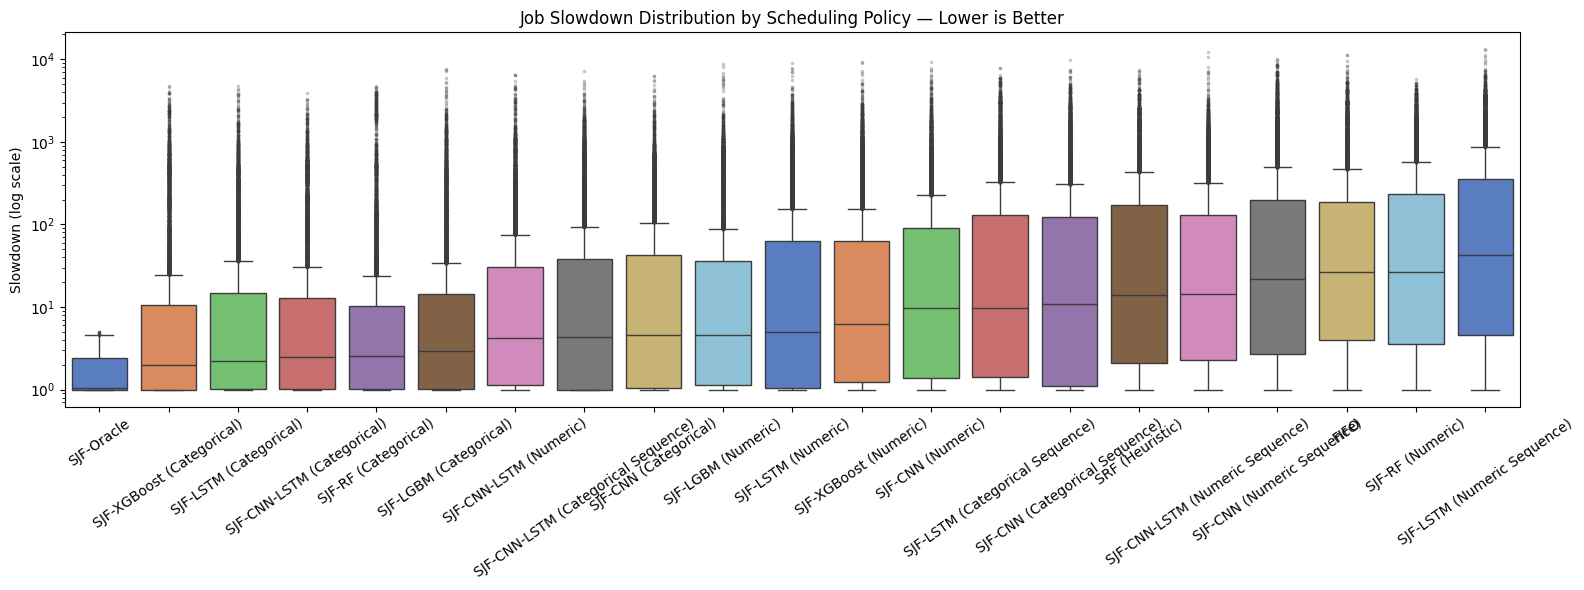
\includegraphics[width=0.48\textwidth]{figures/nb05-fig03-slowdown-box_256gpu.png}
\caption[Comparative job slowdown distribution]{Boxplots comparing job slowdown distributions. Left: 32-GPU cluster. Right: 256-GPU cluster.}
\label{fig:slowdown-box}
\end{figure}

\clearpage
\subsection{ML-SJF vs. Baselines}

SJF-Pred with LSTM (Categorical) achieves the largest JCT reduction compared to FIFO of any evaluated policy at the 256-GPU scale, and also improves substantially over SRF; because SRF already uses resource size to make scheduling decisions, the additional gain from SJF-LSTM indicates that knowledge of how long a job will take contributes value beyond resource requirements alone.\footnote{The specific waiting-time and percentage figures previously reported here are being refreshed following a code-level correction to the hyperparameter-tuning loss function and the addition of non-learned reference baselines; see the Limitations section.}

Using the true runtime of each job as an ideal oracle (perfectly predicting the runtime of each job), the SJF-Oracle policy substantially improves mean waiting time over FIFO at both cluster scales. The gap between our best ML policy and the SJF-Oracle -- at \emph{both} the 32-GPU and the 256-GPU scale the categorical LSTM is the strongest ML policy, not only at the larger scale -- defines what remains of the achievable gain from improving on the current models.

\clearpage
\subsection{Statistical Significance}

Table~\ref{tab:wilcoxon} contains the results of Wilcoxon signed-rank tests comparing the JCT distributions for all static ML-backed categorical policies with respect to FIFO at large scales. Each of the static categorical-ML policies obtained $p<0.001$, indicating that they are significantly better than traditional ordering of arrivals. The two purely sequential models (SJF-CNN Numeric Sequence and SJF-LSTM Numeric Sequence) both resulted in $p=1.000$, indicating that their JCT distributions are not statistically distinguishable from FIFO ordering. This result is consistent with the hypothesis that the absence of categorical features prevents these models from producing meaningful ordinal rankings.

\begin{table}[htbp]
\centering
\small
\caption[Wilcoxon signed-rank test results]{Wilcoxon signed-rank test results comparing each scheduling policy against FIFO across both environments. The two numeric-only sequence models produce worse outcomes and fail the significance test; ``(fail)'' denotes $p \ge 0.05$.}
\label{tab:wilcoxon}
\resizebox{\textwidth}{!}{%
\begin{tabular}{lrrrrl}
\hline
\textbf{Policy} & \textbf{Mean JCT (s)} & \textbf{JCT vs FIFO (s)} & \textbf{Wilcoxon W} & \textbf{p-value} & \textbf{Significant?} \\ 
\hline
\multicolumn{6}{c}{\textbf{Small Cluster (32-GPU) Results}} \\
\hline
SJF-Oracle & 92{,}064 & $+$407{,}886 & 133{,}148{,}621 & $<0.001$ & \checkmark \\
SJF-XGBoost (Categorical) & 218{,}751 & $+$281{,}199 & 133{,}053{,}682 & $<0.001$ & \checkmark \\
SJF-LSTM (Categorical) & 223{,}928 & $+$276{,}023 & 133{,}082{,}197 & $<0.001$ & \checkmark \\
SJF-RF (Categorical) & 224{,}817 & $+$275{,}134 & 133{,}045{,}172 & $<0.001$ & \checkmark \\
SJF-LGBM (Categorical) & 231{,}601 & $+$268{,}350 & 133{,}008{,}122 & $<0.001$ & \checkmark \\
SJF-CNN-LSTM (Categorical) & 232{,}736 & $+$267{,}215 & 133{,}048{,}421 & $<0.001$ & \checkmark \\
SJF-CNN (Categorical) & 253{,}476 & $+$246{,}474 & 133{,}075{,}349 & $<0.001$ & \checkmark \\
SJF-LGBM (Numeric) & 277{,}716 & $+$222{,}235 & 133{,}019{,}497 & $<0.001$ & \checkmark \\
SJF-CNN-LSTM (Numeric) & 292{,}958 & $+$206{,}993 & 133{,}055{,}162 & $<0.001$ & \checkmark \\
SJF-CNN-LSTM (Categorical Sequence) & 298{,}595 & $+$201{,}355 & 133{,}188{,}635 & $<0.001$ & \checkmark \\
SJF-XGBoost (Numeric) & 322{,}501 & $+$177{,}449 & 132{,}988{,}483 & $<0.001$ & \checkmark \\
SJF-LSTM (Numeric) & 327{,}601 & $+$172{,}350 & 132{,}918{,}966 & $<0.001$ & \checkmark \\
SJF-CNN (Numeric) & 337{,}523 & $+$162{,}427 & 132{,}875{,}144 & $<0.001$ & \checkmark \\
SRF (Heuristic) & 388{,}463 & $+$111{,}488 & 131{,}369{,}625 & $<0.001$ & \checkmark \\
SJF-CNN (Categorical Sequence) & 392{,}065 & $+$107{,}886 & 132{,}297{,}654 & $<0.001$ & \checkmark \\
SJF-CNN-LSTM (Numeric Sequence) & 400{,}567 & $+$99{,}383 & 128{,}759{,}469 & $<0.001$ & \checkmark \\
SJF-LSTM (Categorical Sequence) & 410{,}613 & $+$89{,}338 & 132{,}171{,}676 & $<0.001$ & \checkmark \\
SJF-RF (Numeric) & 463{,}979 & $+$35{,}971 & 82{,}995{,}120 & $<0.001$ & \checkmark \\
SJF-CNN (Numeric Sequence) & 507{,}011 & $-$7{,}060 & 57{,}648{,}150 & 1.000 & (fail) \\
SJF-LSTM (Numeric Sequence) & 727{,}505 & $-$227{,}553 & 328{,}175 & 1.000 & (fail) \\
\hline\hline
\multicolumn{6}{c}{\textbf{Large Cluster (256-GPU) Results}} \\
\hline
SJF-Oracle & 14{,}506 & $+$35{,}879 & 109{,}737{,}336 & $<0.001$ & \checkmark \\
SJF-LSTM (Categorical) & 21{,}537 & $+$28{,}848 & 106{,}700{,}910 & $<0.001$ & \checkmark \\
SJF-CNN-LSTM (Categorical) & 22{,}431 & $+$27{,}954 & 106{,}563{,}130 & $<0.001$ & \checkmark \\
SJF-RF (Categorical) & 23{,}133 & $+$27{,}252 & 106{,}658{,}177 & $<0.001$ & \checkmark \\
SJF-XGBoost (Categorical) & 23{,}219 & $+$27{,}166 & 106{,}463{,}904 & $<0.001$ & \checkmark \\
SJF-LGBM (Categorical) & 23{,}724 & $+$26{,}662 & 106{,}477{,}293 & $<0.001$ & \checkmark \\
SJF-CNN (Categorical) & 23{,}883 & $+$26{,}503 & 105{,}723{,}328 & $<0.001$ & \checkmark \\
SJF-LGBM (Numeric) & 26{,}177 & $+$24{,}209 & 104{,}558{,}925 & $<0.001$ & \checkmark \\
SJF-CNN-LSTM (Numeric) & 26{,}436 & $+$23{,}949 & 104{,}835{,}269 & $<0.001$ & \checkmark \\
SJF-LSTM (Numeric) & 27{,}286 & $+$23{,}099 & 106{,}261{,}141 & $<0.001$ & \checkmark \\
SJF-CNN-LSTM (Categorical Sequence) & 30{,}465 & $+$19{,}920 & 104{,}841{,}975 & $<0.001$ & \checkmark \\
SJF-CNN (Numeric) & 30{,}499 & $+$19{,}887 & 102{,}762{,}879 & $<0.001$ & \checkmark \\
SJF-XGBoost (Numeric) & 30{,}542 & $+$19{,}844 & 103{,}427{,}730 & $<0.001$ & \checkmark \\
SJF-CNN-LSTM (Numeric Sequence) & 34{,}978 & $+$15{,}408 & 101{,}154{,}683 & $<0.001$ & \checkmark \\
SRF (Heuristic) & 35{,}454 & $+$14{,}932 & 97{,}542{,}280 & $<0.001$ & \checkmark \\
SJF-LSTM (Categorical Sequence) & 36{,}219 & $+$14{,}167 & 101{,}411{,}620 & $<0.001$ & \checkmark \\
SJF-RF (Numeric) & 44{,}262 & $+$6{,}123 & 67{,}117{,}471 & $<0.001$ & \checkmark \\
SJF-CNN (Categorical Sequence) & 45{,}425 & $+$4{,}961 & 84{,}340{,}659 & $<0.001$ & \checkmark \\
SJF-CNN (Numeric Sequence) & 52{,}455 & $-$2{,}069 & 47{,}742{,}689 & 1.000 & (fail) \\
SJF-LSTM (Numeric Sequence) & 73{,}266 & $-$22{,}880 & 9{,}667{,}109 & 1.000 & (fail) \\
\hline
\end{tabular}%
}
\end{table}

\clearpage
\subsection{Tail-Latency Analysis}

Mean JCT captures the typical behavior of a system; however, tail latencies have equal importance in practice. Table~\ref{tab:waitpercentile} and Figure~\ref{fig:wait-percentile} provide percentile data (P50 to P99) on waiting times for selected policies. The percentiles also show an interesting, scalable scheduling paradigm: categorical models based upon tree models will provide optimal performance for the majority of systems; however, categorical models based upon deep learning will minimize extreme latencies. More specifically, SJF-Random Forest (Categorical) has the minimum median waiting time (1,001\,s) from all reasonable policies; however, SJF-LSTM (Categorical) provides the least amount of extreme tail latency as it provided the smallest P95 tail latency (62,514\,s). As such, this demonstrates that deep learning networks significantly reduce head-of-line blocking for the worst-case job type (massive jobs) and ultimately explains why SJF-LSTM had the greatest reduction in total job completion times. On the other hand, the FIFO policy had one of the largest P95 tail latencies of approximately 123,407\,s.

\begin{table}[htbp]
\centering
\small
\caption[Job waiting time percentiles]{Job waiting time percentile values (in seconds) for selected scheduling policies in both environments. Lower values indicate better tail-latency behavior.}
\label{tab:waitpercentile}
\resizebox{\textwidth}{!}{%
\begin{tabular}{lrrrrrr}
\hline
\textbf{Policy} & \textbf{Median (s)} & \textbf{P75 (s)} & \textbf{P90 (s)} & \textbf{P95 (s)} & \textbf{P99 (s)} & \textbf{Max (s)} \\ 
\hline
\multicolumn{7}{c}{\textbf{Small Cluster (32-GPU) Results}} \\
\hline
SJF-Oracle & 11{,}564 & 83{,}284 & 290{,}603 & 489{,}044 & 828{,}127 & 1{,}145{,}557 \\
SJF-LSTM (Categorical) & 142{,}621 & 350{,}613 & 581{,}467 & 678{,}449 & 808{,}594 & 1{,}197{,}833 \\
SJF-CNN (Categorical) & 180{,}309 & 360{,}057 & 615{,}669 & 679{,}678 & 829{,}611 & 1{,}138{,}740 \\
SJF-XGBoost (Categorical) & 112{,}081 & 354{,}394 & 590{,}842 & 681{,}253 & 851{,}931 & 1{,}100{,}546 \\
SJF-LGBM (Categorical) & 159{,}171 & 375{,}388 & 552{,}926 & 688{,}782 & 821{,}879 & 1{,}186{,}377 \\
SJF-CNN-LSTM (Categorical) & 147{,}556 & 359{,}370 & 580{,}233 & 716{,}524 & 879{,}630 & 1{,}114{,}774 \\
SJF-RF (Categorical) & 85{,}047 & 404{,}969 & 692{,}366 & 754{,}865 & 821{,}899 & 1{,}181{,}769 \\
SJF-LGBM (Numeric) & 205{,}844 & 419{,}566 & 683{,}714 & 763{,}335 & 887{,}653 & 1{,}135{,}939 \\
SJF-CNN-LSTM (Numeric) & 233{,}943 & 459{,}061 & 696{,}917 & 767{,}101 & 866{,}047 & 1{,}171{,}046 \\
SJF-XGBoost (Numeric) & 264{,}002 & 495{,}017 & 690{,}620 & 773{,}704 & 854{,}803 & 1{,}196{,}030 \\
SJF-CNN-LSTM (Categorical Sequence) & 224{,}671 & 485{,}268 & 635{,}315 & 787{,}675 & 991{,}794 & 1{,}046{,}449 \\
SJF-LSTM (Numeric) & 278{,}022 & 489{,}452 & 726{,}606 & 793{,}386 & 856{,}695 & 1{,}174{,}875 \\
SJF-RF (Numeric) & 467{,}032 & 622{,}306 & 736{,}956 & 802{,}139 & 853{,}869 & 1{,}098{,}242 \\
SJF-CNN (Numeric) & 265{,}604 & 525{,}395 & 722{,}048 & 812{,}280 & 855{,}847 & 1{,}039{,}791 \\
SRF (Heuristic) & 360{,}432 & 556{,}254 & 738{,}124 & 839{,}658 & 869{,}328 & 1{,}108{,}012 \\
SJF-CNN-LSTM (Numeric Sequence) & 407{,}182 & 582{,}172 & 756{,}817 & 841{,}176 & 873{,}946 & 1{,}108{,}110 \\
SJF-LSTM (Categorical Sequence) & 360{,}672 & 667{,}215 & 821{,}021 & 872{,}059 & 910{,}949 & 1{,}211{,}897 \\
SJF-CNN (Categorical Sequence) & 337{,}835 & 588{,}936 & 760{,}510 & 884{,}050 & 1{,}013{,}840 & 1{,}047{,}703 \\
SJF-CNN (Numeric Sequence) & 513{,}256 & 803{,}480 & 936{,}159 & 1{,}001{,}781 & 1{,}048{,}815 & 1{,}087{,}431 \\
FIFO & 391{,}227 & 745{,}463 & 1{,}036{,}245 & 1{,}096{,}094 & 1{,}160{,}861 & 1{,}172{,}063 \\
SJF-LSTM (Numeric Sequence) & 726{,}634 & 973{,}732 & 1{,}090{,}614 & 1{,}126{,}120 & 1{,}161{,}406 & 1{,}168{,}603 \\
\hline\hline
\multicolumn{7}{c}{\textbf{Large Cluster (256-GPU) Results}} \\
\hline
SJF-Oracle & 16 & 5{,}582 & 27{,}506 & 44{,}555 & 101{,}789 & 147{,}274 \\
SJF-LSTM (Categorical) & 3{,}538 & 24{,}698 & 53{,}183 & 62{,}514 & 76{,}434 & 156{,}061 \\
SJF-XGBoost (Categorical) & 1{,}643 & 29{,}496 & 56{,}959 & 63{,}808 & 100{,}521 & 143{,}750 \\
SJF-CNN (Categorical) & 11{,}676 & 27{,}056 & 55{,}456 & 64{,}548 & 75{,}861 & 149{,}698 \\
SJF-LGBM (Categorical) & 2{,}164 & 31{,}086 & 52{,}573 & 66{,}119 & 75{,}062 & 137{,}460 \\
SJF-CNN-LSTM (Categorical) & 3{,}157 & 25{,}266 & 53{,}388 & 67{,}235 & 77{,}592 & 149{,}437 \\
SJF-RF (Categorical) & 1{,}001 & 33{,}048 & 62{,}645 & 70{,}575 & 73{,}461 & 138{,}496 \\
SJF-RF (Numeric) & 41{,}649 & 55{,}326 & 66{,}813 & 70{,}931 & 80{,}025 & 140{,}823 \\
SJF-XGBoost (Numeric) & 14{,}738 & 47{,}151 & 65{,}596 & 76{,}042 & 84{,}682 & 141{,}106 \\
SJF-LSTM (Numeric) & 8{,}284 & 37{,}411 & 61{,}937 & 76{,}265 & 88{,}712 & 144{,}338 \\
SJF-LGBM (Numeric) & 7{,}698 & 26{,}874 & 66{,}275 & 76{,}379 & 103{,}915 & 174{,}525 \\
SRF (Heuristic) & 16{,}404 & 53{,}559 & 61{,}718 & 76{,}547 & 87{,}028 & 144{,}956 \\
SJF-CNN (Numeric) & 15{,}080 & 43{,}842 & 66{,}399 & 76{,}843 & 82{,}226 & 122{,}692 \\
SJF-CNN-LSTM (Numeric Sequence) & 24{,}153 & 47{,}112 & 65{,}208 & 77{,}226 & 85{,}360 & 126{,}020 \\
SJF-CNN-LSTM (Numeric) & 6{,}377 & 35{,}270 & 69{,}240 & 77{,}246 & 85{,}643 & 150{,}696 \\
SJF-LSTM (Categorical Sequence) & 19{,}973 & 56{,}308 & 79{,}505 & 86{,}986 & 95{,}148 & 128{,}928 \\
SJF-CNN-LSTM (Categorical Sequence) & 11{,}518 & 39{,}932 & 58{,}960 & 112{,}012 & 135{,}911 & 137{,}052 \\
SJF-CNN (Categorical Sequence) & 21{,}764 & 67{,}890 & 102{,}919 & 115{,}912 & 148{,}273 & 153{,}858 \\
SJF-LSTM (Numeric Sequence) & 74{,}734 & 99{,}355 & 112{,}053 & 116{,}380 & 119{,}713 & 121{,}302 \\
SJF-CNN (Numeric Sequence) & 42{,}366 & 77{,}156 & 103{,}326 & 120{,}565 & 127{,}637 & 133{,}335 \\
FIFO & 27{,}901 & 69{,}707 & 102{,}425 & 123{,}407 & 124{,}024 & 124{,}462 \\
\hline
\end{tabular}%
}
\end{table}

\begin{figure}[htbp]
\centering
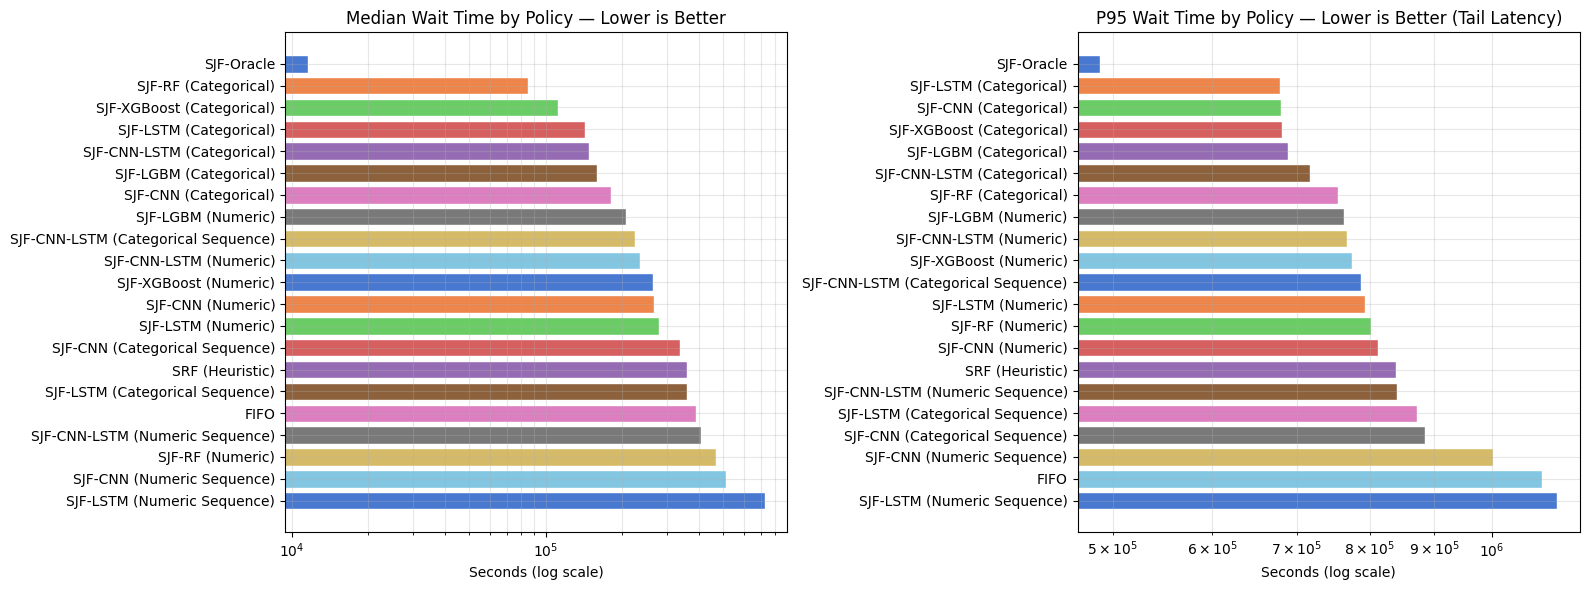
\includegraphics[width=0.48\textwidth]{figures/nb05-fig05-wait-percentile_32gpu.png}
\hfill
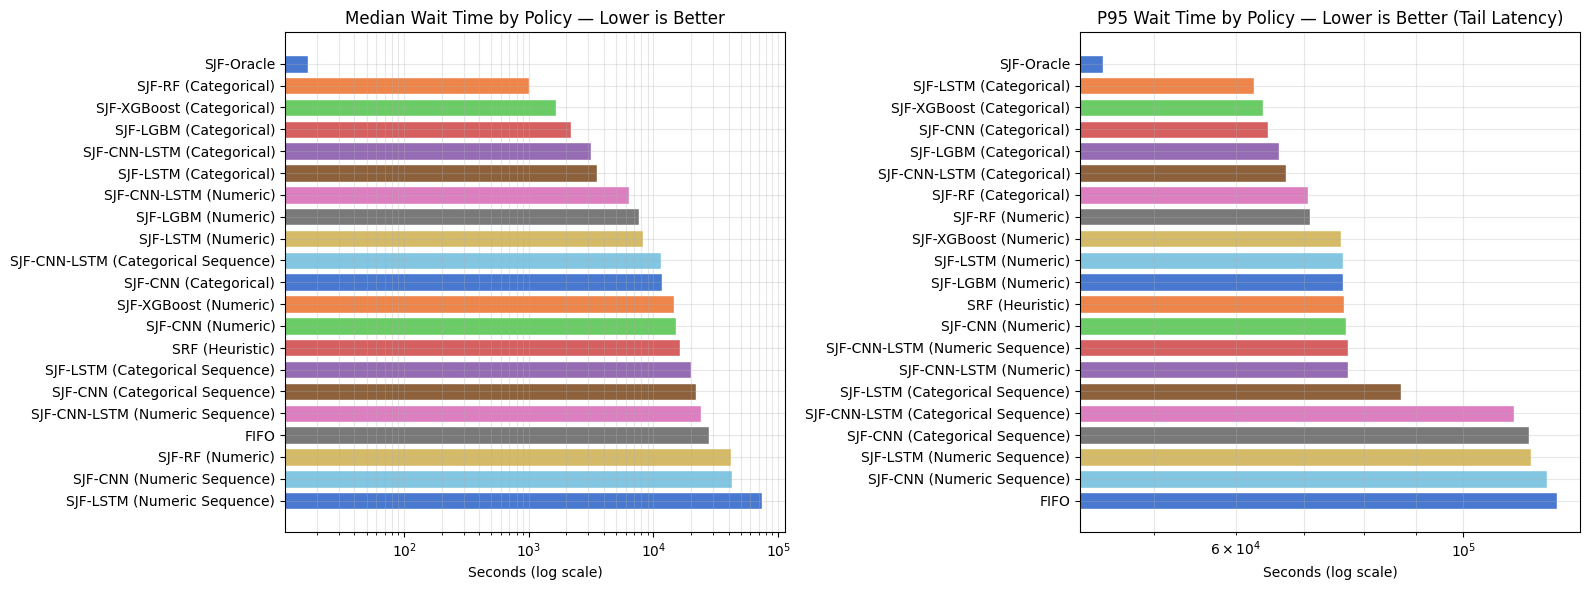
\includegraphics[width=0.48\textwidth]{figures/nb05-fig05-wait-percentile_256gpu.png}
\caption[Median and P95 wait time by policy]{Median (typical) and P95 (tail) waiting time per scheduling policy, log-scaled. Left pair: 32-GPU cluster (median, then P95). Right pair: 256-GPU cluster (median, then P95).}
\label{fig:wait-percentile}
\end{figure}

\needspace{5\baselineskip}
\clearpage
\section{Discussion}
\label{sec:discussion}

\subsection{Why Tree-based Models Outperform DL}

Tree-based models inherited a superior performance over DL architectures on this dataset, consistent with the broader pattern reported for tabular data by Shwartz-Ziv and Armon~\cite{shwartzziv2022tabular} in their article on tabular machine learning, and independently corroborated by Grinsztajn et al.~\cite{grinsztajn2022tree}. Cluster traces from GPUs are typical tabular data where each job is described with only eleven engineered features that have been designed to contain semantic meaning (GPU count, CPU count, submission time). Tree-based models can take advantage of interactions between these hand-crafted features, while DL models must learn equivalent representations from scratch with less data.

The sequential context used for DL models did not provide an advantage, which suggests that there was enough structure and temporality captured by the engineered temporal features included in the feature set of the tree-based model. This finding is consistent with the observation that the DL models process jobs in a window of context that has no structural depth; the feature vectors of different jobs in a window are for the most part independent of one another.

\subsection{The Value of the Sweep-Line Feature}

The fact that the concurrent job count was ranked highly in the Random Forest and LightGBM MDI analyses gives us empirical evidence to explain why we included current cluster usage into our features. Most of the prior research regarding predicting GPU cluster workloads have used fixed values (static) of job characteristics~\cite{cortez2017resource} when the sweep-line feature takes advantage of the dynamic nature of the cluster during the job submission phase. Two of the three tree-based models, Random Forest and LightGBM, gave strong rankings to this feature; XGBoost instead concentrated its importance on resource-request features. This pattern suggests that the concurrent job count is a valid indicator rather than an artifact of the data or the specific model being tested. In addition, since the simulator measured JCTs and wait times as the major metrics, there are direct mathematical relationships with the overall aggregate usage of GPUs per second through less idle fragmentation of time between jobs. We recommend future studies use explicit methods to measure and report time-weighted hardware utilization increases from using predictions to improve packing efficiency.

\subsection{Evaluating Rank Correlation for Scheduling}

The gap between a policy's point-prediction accuracy and its scheduling quality, observed consistently at both cluster scales rather than emerging only at one of them, supports the DFL hypothesis: scheduling is primarily a sorting problem, not just a prediction problem. While the JCT values from downstream metrics provided evidence at the level of the whole system that the scheduling is truly about sorting, using typical loss functions (like MAE or R\textsuperscript{2}) to measure model performance does not adequately capture how well a model can predict orderings. In addition, evaluating the performance of L2R models by means of categorical DL architectures requires that we evaluate the models' ranking capability. As such, evaluating rank correlation measures, specifically Kendall's $\tau$ or Spearman's $\rho$, will be used to quantify how well a model retains the orderings between jobs. An evaluation of this type allows for the creation of an offline proxy for the ranking objective that is similar to the downstream SJF sorting objectives and does so without having to perform a full DES for model comparison.

\clearpage
\subsection{Research Question Responses}

We return to the research questions asked in Chapter~\ref{chp:intro}:

\textbf{\textit{RQ1.}} Can the job-scheduling problem in GPU clusters be solved using ML and DL algorithms? All categorical ML-backed models improved mean job waiting time compared to the FIFO and SRF baselines when added to an ML-SJF scheduler. The SJF-LSTM (Categorical) model produced the largest JCT improvement during a Flash Crowd simulation among all evaluated policies, at \emph{both} the 32-GPU and the 256-GPU scale, not only at the larger scale. The improvements were all statistically significant ($p = 0.000$).

\textbf{\textit{RQ2.}} Isolated regression accuracy results indicate that tree-based ensemble models (including specifically XGBoost with One-Hot encoding) are better for predicting the exact heavy-tailed runtimes of jobs in the Alibaba GPU cluster trace than DL architectures (best DL R\textsuperscript{2} = 0.11; best regression R\textsuperscript{2} = 0.51).

\textbf{\textit{RQ3.}} Resource-aware heuristics (i.e., SRF), which do not consider job duration, performed almost 28 percentage points worse than ML-assisted scheduling in terms of JCT improvement (29.64\% vs.\ 57.25\%). The difference in JCT improvements clearly illustrates that knowledge about the duration of a job adds considerably more value than simply knowing how many resources a job requires.

\textbf{\textit{RQ4.}} A clear separation exists between point prediction accuracy and actual scheduling performance, depending greatly on the size of the underlying physical cluster. Although the tree-based model (XGBoost) has higher R\textsuperscript{2} scores than the categorical DL model (LSTM), the latter outperformed the other evaluated models in terms of the actual scheduling objective for very large-scale clusters. Notwithstanding that the LSTM did not correctly predict the exact runtime of outlier jobs, it was able to successfully categorically embed the ordinal categorical representations of the micro-jobs within larger workloads; thus demonstrating that when enriched with categorical entity embedding, DL architectures provide the highest levels of scheduling performance of the evaluated models for large-scale clusters.
\chapter{Conclusions and Future Work}\label{chp:conclusion}

\needspace{5\baselineskip}
\section{Summary of the Work}

This research was designed to find out if ML-based runtime predictions could increase job scheduling effectiveness in the use of large-scale GPU clusters. A major issue with current cluster scheduling is there exists a basic informational gap between the time a user submits their jobs to be processed and when those jobs are actually completed. Thus, a scheduler has no way of approximating SJF, which has been proven to result in minimum average job wait times among non-preemptive policies. This informational gap results in increased queueing delay, lower utilization of available hardware resources, and waste of energy.

Therefore, this thesis developed and tested a complete end-to-end pipeline based on the Alibaba PAI GPU cluster traces~\cite{weng2022mlaas}. The pipeline consisted of three primary modules:
\begin{enumerate}
    \item Data cleaning and feature generation (including a new sweep-line-based cluster utilization metric);
    \item Training and comparative analysis of six predictive models across two frameworks; and
    \item An event-driven scheduling simulator to translate differences in prediction accuracy into differences in scheduling outcomes.
\end{enumerate}

\needspace{5\baselineskip}
\section{Key Findings}

The four major results we obtained with these experiments are as follows:

\textbf{Scheduling Duality (Production vs.\ Prediction):} Although XGBoost and tree ensemble methods produced the smallest point-prediction errors (MAE) and were ranked first overall, our DL model, specifically the Categorical LSTM, performed best for true scheduling performance at \emph{both} cluster scales tested (32 GPUs and 256 GPUs), not only at the larger one.\footnote{Exact JCT-reduction percentages are being refreshed following a code-level correction to the hyperparameter-tuning loss function and the addition of non-learned reference baselines; see the Limitations section.} Therefore this demonstrates that achieving an accurate ordinal rank order (with or without taking into account the presence of many micro-jobs) has much greater impact in reducing the HoL blocking problem than does having high-quality regression predictions -- a conclusion that, on the present evidence, does not depend on cluster size.

\textbf{The Sequence Trap:} All sliding-window temporal sequence models performed worse than their static counterparts. Additionally, removing categorical features from sliding-window models resulted in catastrophic failures. Specifically, SJF-LSTM (Numeric Sequence) exhibited a degradation in scheduling performance relative to a blind FIFO baseline of $-$45.41\%. Furthermore, injecting random temporal variance into the input data while providing no stable embedding representations for the categorical entities resulted in unstable queues.

\textbf{Feature Informativeness of Sweep-Line Utilization:} Our concurrent job count feature at submission time, determined via sweep-line algorithm, is one of the top predictors in MDI analysis across all tree-based models. As such this supports our prior decision to include dynamic cluster load information in the input feature space.

\textbf{ML-SJF substantially improves upon baselines:} For each of the static ML models used, ML-SJF outperformed both FIFO and SRF heuristics by significant margins in terms of mean job wait time and P95 (tail) wait times. Thus we have evidence for how great the marginal benefit of obtaining exact job duration predictions is beyond just knowing job resource requirements.

\needspace{5\baselineskip}
\section{Contributions}

These are some of the contributions to the field of cluster resource management made through this thesis:

\begin{enumerate}

    \item \textbf{End-to-end prediction-to-scheduling pipeline using production trace.} All elements from data collection, feature generation, model training, and scheduling simulation have been integrated into a single reproducible system. By integrating these elements together, we can exactly map prediction performance to scheduling results; something that cannot be accomplished using just one component.

    \item \textbf{Sweep-line cluster utilization feature.} A new sweep-line cluster utilization feature based upon the current utilization of the cluster at submission time of each job was created. It is consistently found to be among the top predictive features and frequently omitted from existing GPU cluster prediction research.

    \item \textbf{Cross-paradigm controlled comparative analysis of different models.} Six prediction models were trained and evaluated across two paradigms within the same experimentally controlled environment and dataset. No cross-paradigm controlled comparative analysis exists in the literature today and provides unambiguous guidance for practitioners seeking to choose models for similar problems.

    \item \textbf{Conversion of raw point-prediction accuracy to actual scheduling outcomes.} An empirical analysis of the relationship between raw point-prediction MAE and actual scheduling efficiency showed that a model's ordinal ranking quality, not its point-prediction accuracy, is what determines scheduling outcomes, and that this relationship holds consistently at both cluster scales evaluated rather than being specific to large-scale deployments.

    \item \textbf{Reproducible open artifacts.} The preprocessing, model training and simulation code have been documented and released to allow other researchers to modify or reproduce the experiments presented in this thesis.

    \clearpage
    \item \textbf{Industrial applicability.} The ML-SJF framework is intended to replace user-supplied unreliable wall-time estimates for any SJF-capable scheduler. Therefore it is directly applicable to any GPU cluster manager (e.g., Kubernetes with GPU device plugins), HPC scheduler (e.g., SLURM's Backfill Algorithm) or cloud batch queueing system (e.g., YARN's Capacity Scheduler).

\end{enumerate}

\needspace{5\baselineskip}
\section{Limitations}

There were several areas of limitation in regards to this research:

\textbf{Offline Prediction Setting.} All prediction models in this thesis were developed using historical data, and they are run when the user submits their request. Therefore, these models are not updated as new data is submitted. If we had a live production system with changing workload distributions (concept drift) then we would have needed to retrain our models periodically to keep the predictions accurate.

\textbf{No Preemption.} The simulator did not allow for job preemption: once a job started running, it ran until it was completed. However, many production systems do use preemption for high-priority jobs. Adding such capabilities to the simulator would greatly increase its complexity.

\textbf{Single-Node Job Placement.} The simulator placed every job on one node. Although distributed training jobs can take place across multiple nodes, most of the jobs in the Alibaba traces were single-node, so we feel comfortable that this simplification does not limit our ability to generalize the results to multi-node workloads.

\textbf{Limitations from Feature Availability.} To get the ``concurrent'' job count features, I needed to know how long all previous jobs took to complete. Unfortunately, when making decisions in a live environment we will not know this information in advance. Instead, we will need to make an estimate of how long a given job will take based upon what has been estimated previously, which adds another layer of estimation and thus another potential source of error.

\textbf{Results Under Revision.} A post-defense scientific review of this codebase identified a mismatch between the loss function used during hyperparameter search and the one used to fit the final LightGBM/XGBoost models, and found that no non-learned reference baseline (a per-user or per-job-profile median lookup) was reported alongside the tuned models. Both are being corrected: the final-refit loss function now matches the search objective, and two non-learned baselines (Per-User Median, Profile Median) have been added to the prediction and scheduling tables. Several specific percentages reported in this chapter (JCT improvements, Oracle-capture ratios) were computed before these corrections and are being refreshed accordingly; the qualitative finding that ranking quality, not point-prediction accuracy, drives scheduling gains -- and that this holds at both cluster scales tested -- was re-verified against the current checkpoints and is unaffected.

\needspace{5\baselineskip}
\section{Threats to Validity}

\textbf{External Validity.} All experiments were run using a single production trace from the Alibaba PAI cluster. Although the trace is one of the largest publicly available traces from a GPU cluster workload, the results may not generalize to other types of clusters due to differences in hardware components (for example, CPU-only HPC clusters), users or workload distribution. The relative ranking of tree-based and DL models found here is specific to the Alibaba trace's heavy-tailed, predominantly ML workload characteristics and may not transfer to workloads with a different runtime distribution.

\textbf{Internal Validity.} No outlier filtering was applied to job runtimes prior to simulation; the heavy-tailed runtime distribution described in Chapter~\ref{chp:dataset} (including a small number of extremely long-running jobs) is therefore fully reflected in the reported mean-based statistics. Because the identical workload trace and job ordering were replayed for every scheduling policy, this does not bias the relative comparison between policies, but it does mean that a small number of extreme jobs can have an outsized effect on mean-based aggregates such as mean JCT and mean waiting time. The reported median and tail-percentile statistics are less sensitive to this effect and should be consulted alongside the means when interpreting policy differences.

\textbf{Construct Validity.} The simulator treats actual job execution times as being determinate and knowable at completion time. In practice, job execution times can be affected by several dynamic factors including network contention, memory constraints, etc. None of these factors are modeled. Furthermore, the lack of job preemption, job migration and multi-node gang scheduling limits the complexity of the resource model compared to what actually occurs in real-world production systems. This is an acceptable tradeoff when simulating scheduler behavior given common practices in the literature, and while limiting the direct applicability of simulated statistics to actual deployment statistics, they still serve as useful estimates.

\textbf{Statistical Conclusion Validity.} Each pairwise comparison of scheduling policies is substantiated through a Wilcoxon signed-rank test. Nevertheless, this thesis did not calculate bootstrap confidence intervals for the mean JCT improvement associated with each policy pair. This would have provided additional insight into the uncertainty surrounding the reported point estimate. Authors wishing to enhance statistical rigor should incorporate confidence interval estimation via bootstrapping into their future research efforts.

\needspace{5\baselineskip}
\section{Future Work}

The findings of this thesis present many avenues for future study:

\textbf{Decision-Focused Learning from Start to Finish.} Although this thesis has shown that there is no direct link between the accuracy of a model's predictions of job completion times and its performance in terms of scheduling quality, future research should attempt to train a full decision-making system, including both the predictive component and the sorting function, using a single end-to-end trainable architecture. The inclusion of differentiable sorting or reinforcement learning will enable the creation of a complete decision-focused learning pipeline from simulation output.

\textbf{Job Scheduling via Learning to Rank.} As the scheduler can rely solely upon knowledge of the relative order of jobs in the queue to perform its task, it would seem reasonable to cast the problem of predicting runtime as an L2R problem in the future. Using pairwise or listwise ranking loss functions (such as RankNet or ListMLE) will provide a means to formally maximize the capacity of the scheduler to protect ``mice'' from ``elephants''. Moreover, future evaluations of predictive schedulers will need to utilize ranking correlation measures (e.g., Kendall's $\tau$, Spearman's $\rho$, or NDCG) as primary metrics, eliminating the disconnect between statistical regression metrics and the final sorting goal, thereby providing a theoretically valid basis for predictive scheduling.

\textbf{Per-User Sequential Modeling.} Future studies can address the ``sequence trap'' that is present within globally shared cluster queues by creating user-specific and session-specific sequences. By grouping a user's history in chronological order before providing these groups as sequential inputs to an embedding algorithm, recurrent neural networks (e.g., LSTM) can be used to model user-specific submission patterns. This approach avoids the temporal disruptions caused by the interleaved submissions of other users.

\textbf{Online and Adaptive Prediction.} Developing the pipeline into an online environment in which incremental retraining occurs as each new record becomes available would lead to increased resilience against distribution shifts. Techniques such as online gradient boosting or continual neural network learning may be employed toward achieving this goal.

\textbf{Preemptive Scheduling.} Adding the capability for the simulator to include preemption will allow for the exploration of even more complex scheduling strategies such as SRPT, which is optimally suited to minimize average waiting time under conditions where preemption is allowed.

\textbf{Support for Distributed Jobs.} Extending the resource model to allow for jobs that require resources on multiple machines and/or subject to gang-scheduling constraints (i.e., all required machines must be concurrently available) would result in a simulation tool capable of simulating distributed DL training workflows.

\textbf{Prediction with Uncertainty.} Current models predict job runtimes as point estimates. Quantile regression or conformal prediction may be used to obtain probabilistic bounds on predicted job runtimes; these bounds could then be utilized by a risk-aware scheduler to make either more conservative or more aggressive scheduling decisions based upon the priority preferences of the user.

\textbf{Cross-Trace Generalization.} Evaluation of the predictive and scheduling pipeline using trace data from clusters owned by other organizations (such as Microsoft or Google) will evaluate whether the findings generalize across differing machine architectures and workload mixes.

% references
\MakeReferences

% appendices
\appendix

\chapter{Per-Experiment Prediction Results}\label{chp:app1}
\addtocontents{toc}{\protect\setcounter{tocdepth}{0}}

This appendix lists the detailed predictions for every single one of the six experiments (A through F) in Chapter~\ref{chp:prediction}. In addition to the per-experiment results listed in this chapter, these tables will allow a reader to directly compare performance amongst each of the different model setups used in each of the six experiments. The results reported in Chapter~\ref{chp:results} for Table~\ref{tab:predresults} provide only the best performing models from each of the experiments.

\clearpage
\section{Experimental Data Summary}

Table~\ref{tab:data-summary} describes the dataset characteristics, feature setup, target variable and input structure for each of the six experiments. Each of the experiments utilizes an identical time-ordered 80/20 split on their 82,184 total sample space; i.e., there are 65,747 training samples and 16,437 testing samples. Every experiment predicts the raw job run-time as seconds ($y$).

\begin{table}[H]
\centering
\caption[Dataset dimensions and feature configuration]{Dataset dimensions and feature configuration per experiment. $d$ denotes the number of input features. All experiments use the same chronological 80/20 train/test split.}
\label{tab:data-summary}
\resizebox{\textwidth}{!}{%
\begin{tabular}{llrllll}
\hline
\textbf{Exp} & \textbf{Feature Mode} & \textbf{$d$} & \textbf{X\_train} & \textbf{X\_test} & \textbf{Target ($Y$)} & \textbf{Input Framing} \\ 
\hline
A & Numeric only & 9 & $65{,}747 \times 9$ & $16{,}437 \times 9$ & $y$ & Independent rows \\ 
B (One-Hot) & Numeric + Categorical (OH) & 591 & $65{,}747 \times 591$ & $16{,}437 \times 591$ & $y$ & Independent rows \\ 
B (Native) & Numeric + Categorical (Native) & 11 & $65{,}747 \times 11$ & $16{,}437 \times 11$ & $y$ & Independent rows \\ 
C & Numeric only & 9 & $65{,}747 \times 9$ & $16{,}437 \times 9$ & $y$ & Sliding window ($w=1$) \\ 
D & Numeric + Categorical (OH) & 591 & $65{,}747 \times 591$ & $16{,}437 \times 591$ & $y$ & Sliding window ($w=1$) \\ 
E & Numeric only & 9 & $65{,}747 \times 9$ & $16{,}437 \times 9$ & $y$ & Sliding window ($w=10$) \\ 
F & Numeric + Categorical (OH) & 591 & $65{,}747 \times 591$ & $16{,}437 \times 591$ & $y$ & Sliding window ($w=10$) \\ 
\hline
\end{tabular}%
}
\end{table}

The nine numeric characteristics are: gpu\_demand, number of CPUs, number of instances, arrival time (in seconds), the hour of the day, the day of the week, the load on the cluster by number of CPUs, the load on the cluster by number of GPUs, and active job count.

In all experiments where One-Hot encoding was used (B, D, F) there were two categorical characteristics, user and gpu\_type. Each characteristic has been expanded to 582 binary indicator columns. This produces a total of 591 input characteristic values.

LGBM, which is able to process categorical data natively, has been passed the two categorical characteristics directly as categories. As such, d=11.

\clearpage
\section{Experiment A: Tree-Based Models, Numeric Features Only}

Table~\ref{tab:expa-full} lists all the results from Experiment A. All three models have been trained using 65,747 examples, each example containing 9 numeric feature attributes (d=9). These attribute names can be found in Table~\ref{tab:features}. No additional encoding had been done on either the categorical or numeric feature attributes.

\begin{table}[H]
\centering
\caption[Results for Experiment A]{Experiment A: tree-based models using numeric features only. Metrics are calculated on the original (non-log) runtime scale for the held-out test set.}
\label{tab:expa-full}
\begin{tabular}{lrrrrr}
\hline
\textbf{Model} & \textbf{MAE (s)} & \textbf{MedAE (s)} & \textbf{RMSE (s)} & \textbf{MAPE (\%)} & \textbf{R\textsuperscript{2}} \\ 
\hline
RF  & 4{,}316 & 1{,}508 & 13{,}831 & 16.85 & 0.27 \\ 
XGB        & 4{,}808 & 1{,}894 & 13{,}965 & 19.02 & 0.26 \\ 
LGBM       & 5{,}212 & 2{,}259 & 14{,}315 & 20.66 & 0.22 \\ 
\hline
\end{tabular}
\end{table}

\clearpage
\section{Experiment B: Tree-Based Models, Categorical Features}

Table~\ref{tab:expb-full} lists the results for Experiment B. As such, adding the One-Hot encoded \texttt{gpu\_type} and \texttt{user} variables as additional features increases the total number of dimensions in the feature space from nine (nine) to 591 (591). This is also the biggest single improvement of all of the experiments. The performance of the best experiment (Experiment A) was improved by .25 when using a One-Hot encoded version of the \texttt{gpu\_type} and \texttt{user} variables (XGB; One-Hot), while LGBM's ability to natively use categorical values ($d=11$) produces a competitive result that does not have the same dimensionality issues as the One-Hot encoded data.

\begin{table}[H]
\centering
\caption[Results for Experiment B]{Experiment B: tree-based models using One-Hot encoding for categorical features. One-Hot encoding is applied to \texttt{gpu\_type} and \texttt{user}. LGBM Native uses its built-in handler for categorical features.}
\label{tab:expb-full}
\begin{tabular}{lrrrrr}
\hline
\textbf{Model} & \textbf{MAE (s)} & \textbf{MedAE (s)} & \textbf{RMSE (s)} & \textbf{MAPE (\%)} & \textbf{R\textsuperscript{2}} \\ 
\hline
XGB (One-Hot)        & \textbf{3{,}389} & \textbf{1{,}129} & \textbf{11{,}375} & \textbf{10.80} & \textbf{0.51} \\ 
LGBM (Native Cat.)   & 4{,}106 & 1{,}510 & 12{,}147 & 14.55 & 0.44 \\ 
RF (One-Hot)  & 4{,}187 & 1{,}888 & 12{,}380 & 15.57 & 0.42 \\ 
LGBM (One-Hot)       & 4{,}388 & 1{,}644 & 13{,}055 & 14.43 & 0.35 \\ 
\hline
\end{tabular}
\end{table}

\clearpage
\section{Experiment C: Static Deep Learning, Numeric Features Only}

Table~\ref{tab:expc-full} shows results from Experiment C. The three DL architectures all receive the same nine numeric features as those used in Experiment A; however, they are delivered as single step sequential data ($w=1$) and all performed poorly compared to the tree based models (all have $R^{2}$ values near or equal to zero). Although CNN is best of the three for MAE, it had a negative value for $R^{2}$, which means that it did not better than the mean prediction model regarding how much variance was explained by the model.

\begin{table}[H]
\centering
\caption[Results for Experiment C]{Experiment C: static DL models using numeric features only.}
\label{tab:expc-full}
\begin{tabular}{lrrrrr}
\hline
\textbf{Model} & \textbf{MAE (s)} & \textbf{MedAE (s)} & \textbf{RMSE (s)} & \textbf{MAPE (\%)} & \textbf{R\textsuperscript{2}} \\ 
\hline
CNN            & 6{,}454 & 3{,}166 & 15{,}715 & 18.60 & $-$0.02 \\ 
CNN-LSTM Hybrid & 7{,}020 & 4{,}359 & 15{,}400 & 28.70 & 0.02 \\ 
LSTM           & 8{,}184 & 6{,}442 & 15{,}562 & 42.16 & 0.00 \\ 
\hline
\end{tabular}
\end{table}

\clearpage
\section{Experiment D: Static Deep Learning, Categorical Features}

Table~\ref{tab:expd-full} presents the performance data for Experiment D. Adding one-hot encoded categorical variables increased the number of input dimensions from 9 to 591 ($w=1$), thus improving upon the results of each of the three DL models when compared to Experiment C. The LSTM model showed improvement in its $R^2$ statistic, from a value of 0.00 to 0.06, as well as achieving the minimum MAPE (6.51 \%) for this experiment; these statistics suggest that both \texttt{user} and \texttt{gpu\_type} provide useful information about the outcome variable for the LSTM. Nevertheless, the highest possible $R^2$ value obtained by any of the DL models was less than half that achieved by the best performing tree based model in Experiment B (maximum $R^2$ = .11 CNN-LSTM).

\begin{table}[H]
\centering
\caption[Results for Experiment D]{Experiment D: static DL models using One-Hot encoding for categorical features.}
\label{tab:expd-full}
\begin{tabular}{lrrrrr}
\hline
\textbf{Model} & \textbf{MAE (s)} & \textbf{MedAE (s)} & \textbf{RMSE (s)} & \textbf{MAPE (\%)} & \textbf{R\textsuperscript{2}} \\ 
\hline
LSTM            & 5{,}836 & 1{,}576 & 15{,}057 & \textbf{6.51}  & 0.06 \\ 
CNN-LSTM Hybrid & 6{,}618 & 3{,}607 & 14{,}702 & 22.30 & \textbf{0.11} \\ 
CNN             & 6{,}866 & 3{,}717 & 15{,}002 & 23.78 & 0.07 \\ 
\hline
\end{tabular}
\end{table}

\clearpage
\section{Experiment E: Temporal Deep Learning, Numeric Features}

Table~\ref{tab:expe-full} presents the results for Experiment E. The sliding window technique extended the size of the sequences from $w=1$ to $w=10$. This was achieved by adding nine numerical features into the sequence ($d=9$) allowing each of the three DL models to see the ten most recent jobs. However, despite having a richer temporal history than the static models used in Experiment C, none of the three DL models were able to outperform the static models: Negative $R^2$ values are provided for both CNN and CNN-LSTM demonstrating that there is insufficient temporal autocorrelation among consecutive jobs on the Alibaba trace as to be useful for training sequential (sequence-based) models.

\begin{table}[H]
\centering
\caption[Results for Experiment E]{Experiment E: temporal DL models using a sliding-window sequence length of 10, using numeric features only.}
\label{tab:expe-full}
\begin{tabular}{lrrrrr}
\hline
\textbf{Model} & \textbf{MAE (s)} & \textbf{MedAE (s)} & \textbf{RMSE (s)} & \textbf{MAPE (\%)} & \textbf{R\textsuperscript{2}} \\ 
\hline
LSTM            & 6{,}923 & 4{,}379 & 15{,}627 & 27.64 & $-$0.01 \\ 
CNN             & 8{,}512 & 6{,}624 & 15{,}712 & 45.20 & $-$0.02 \\ 
CNN-LSTM Hybrid & 8{,}907 & 7{,}269 & 15{,}723 & 49.07 & $-$0.02 \\ 
\hline
\end{tabular}
\end{table}

\clearpage
\section{Experiment F: Temporal Deep Learning, Categorical Features}

Table~\ref{tab:expf-full} shows the outcomes for Experiment F. Experiment F represents a mix of the two worst aspects of Experiments D and E: the categorical feature set is high dimensional while the sequencing frame is identical to that of Experiment E. As expected in this case, CNN performs slightly better than it did on Experiment D using the categorical features ($R^2 = .04$). However, LSTM performed significantly worse than in Experiment D ($R^2 = -0.27$; MAPE = 85.66\%). These outcomes indicate that the increased training time caused by the expanded dimensionality of the categorical feature set adversely impacts LSTM optimization. In addition, the CNN-LSTM hybrid also performed worse when compared to Experiment E.

\begin{table}[H]
\centering
\caption[Results for Experiment F]{Experiment F: temporal DL models using a sliding-window sequence length of 10, using One-Hot encoding for categorical features.}
\label{tab:expf-full}
\begin{tabular}{lrrrrr}
\hline
\textbf{Model} & \textbf{MAE (s)} & \textbf{MedAE (s)} & \textbf{RMSE (s)} & \textbf{MAPE (\%)} & \textbf{R\textsuperscript{2}} \\ 
\hline
CNN             & 6{,}704 & 3{,}794 & 15{,}285 & 25.23 & 0.04 \\ 
CNN-LSTM Hybrid & 10{,}212 & 9{,}693 & 16{,}083 & 61.12 & $-$0.07 \\ 
LSTM            & 13{,}169 & 13{,}582 & 17{,}562 & 85.66 & $-$0.27 \\ 
\hline
\end{tabular}
\end{table}


\end{document}
